\documentclass[aspectratio=169]{beamer}

\usetheme{Madrid}
\usecolortheme{default}

\usepackage[T1]{fontenc}
\usepackage[utf8]{inputenc}
\usepackage{graphicx}
\usepackage{booktabs}
\usepackage{tikz}
\usepackage{hyperref}
\usepackage{amsmath}

\usetikzlibrary{arrows.meta,positioning,shapes.geometric,fit,calc}

\title{TCP RTO Improvement and EL-RTO Evaluation in ns-3}
\subtitle{Supervisor Briefing for Student ID 2105114}
\author{Student ID: 2105114}
\date{\today}

\begin{document}

\begin{frame}
  \titlepage
\end{frame}

\begin{frame}{Presentation Roadmap}
  \tableofcontents
\end{frame}

\section{Overview}
\begin{frame}{Project Scope}
  \begin{itemize}
    \item Objective: compare three TCP retransmission-timeout behaviors in ns-3.
    \item Modes evaluated:
    \begin{itemize}
      \item Standard Jacobson RTT/RTO estimator
      \item Improved adaptive Xiao-Zhang estimator
      \item EL-RTO: improved estimator with spike suppression
    \end{itemize}
    \item Checklist assignment mapping:
    \[
      2105114 \bmod 8 = 2
    \]
    \item Required wireless cases:
    \begin{itemize}
      \item Wireless 802.11 (mobile)
      \item Wireless 802.15.4 (mobile)
    \end{itemize}
  \end{itemize}
\end{frame}

\section{Implementation}
\begin{frame}{Main Files Changed or Added}
  \textbf{Core ns-3 timer logic}
  \begin{itemize}
    \item \texttt{src/internet/model/rtt-estimator.h}
    \item \texttt{src/internet/model/rtt-estimator.cc}
  \end{itemize}

  \textbf{Main wireless checklist experiment}
  \begin{itemize}
    \item \texttt{scratch/rto-checklist-wireless.cc}
  \end{itemize}

  \textbf{Base-paper and EL-RTO experiments}
  \begin{itemize}
    \item \texttt{scratch/rto-smooth-simulation.cc}
    \item \texttt{scratch/rto-elrto-spike-simulation.cc}
  \end{itemize}

  \textbf{Automation and plotting}
  \begin{itemize}
    \item \texttt{run-selected-checklist.py}
    \item \texttt{run-wifi-mobile-10s.py}
    \item \texttt{run-lrwpan-mobile-10s.py}
    \item \texttt{plot-checklist-wireless.py}
    \item \texttt{plot-results.py}
    \item \texttt{plot-elrto-spike.py}
  \end{itemize}
\end{frame}

\begin{frame}{What Changed in \texttt{rtt-estimator}}
  \begin{itemize}
    \item Added mode control attributes:
    \begin{itemize}
      \item \texttt{UseAdaptive}
      \item \texttt{UseElRto}
      \item \texttt{ElRtoWindow}
      \item \texttt{ElRtoTheta}
    \end{itemize}
    \item Added adaptive RTT change-rate logic:
    \[
      k = \left| \frac{RTT_n - RTT_{n-1}}{RTT_{n-1}} \right|
    \]
    \item Added adaptive weight update:
    \[
      \alpha_n = \alpha_0 (1 + k), \qquad \beta_n = \beta_0 (1 - k)
    \]
    \item Added EL-RTO spike suppression using a recent RTT window.
    \item Added synchronized logging of RTT, SRTT, RTTVAR, and RTO after each estimator update.
  \end{itemize}
\end{frame}

\begin{frame}{Why These Timer Changes Were Needed}
  \begin{itemize}
    \item Stock ns-3 provides the standard Jacobson-style estimator only.
    \item The project required a direct comparison between:
    \begin{itemize}
      \item standard mode
      \item improved adaptive mode
      \item EL-RTO mode
    \end{itemize}
    \item Adaptive mode was added to make SRTT react faster when RTT changes rapidly.
    \item EL-RTO was added to avoid over-inflating RTTVAR and RTO during short-lived RTT spikes.
    \item Unified logging was added so every plotted CSV row is internally consistent.
  \end{itemize}
\end{frame}

\section{Topologies}
\begin{frame}{Base Paper Reproduction Topology}
  \centering
  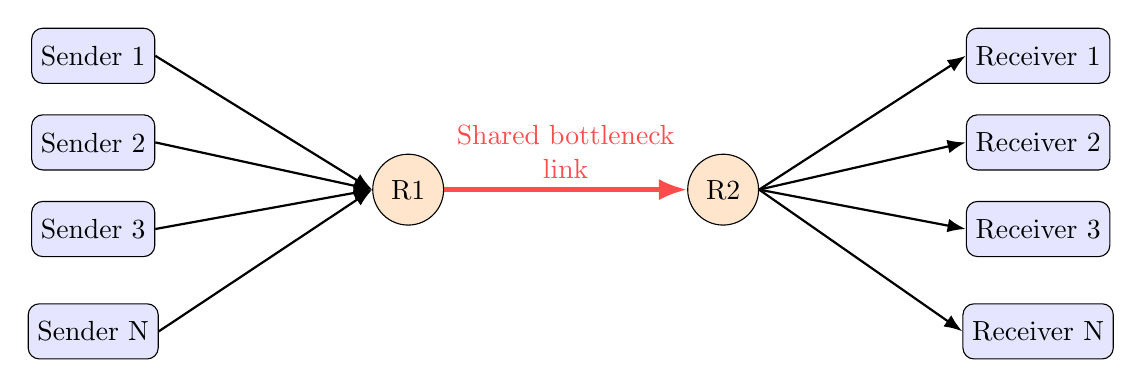
\begin{tikzpicture}[
    node distance=0.7cm and 1.2cm,
    host/.style={draw, rounded corners, minimum width=1.55cm, minimum height=0.7cm, fill=blue!10},
    router/.style={draw, circle, minimum size=0.9cm, fill=orange!20},
    link/.style={-Latex, thick},
    bottleneck/.style={-Latex, ultra thick, red!70}
  ]
    \node[host] (s1) at (0,2.2) {Sender 1};
    \node[host] (s2) at (0,1.1) {Sender 2};
    \node[host] (s3) at (0,0.0) {Sender 3};
    \node[host] (sn) at (0,-1.3) {Sender N};

    \node[router] (r1) at (4,0.5) {R1};
    \node[router] (r2) at (8,0.5) {R2};

    \node[host] (d1) at (12,2.2) {Receiver 1};
    \node[host] (d2) at (12,1.1) {Receiver 2};
    \node[host] (d3) at (12,0.0) {Receiver 3};
    \node[host] (dn) at (12,-1.3) {Receiver N};

    \draw[link] (s1.east) -- (r1.west);
    \draw[link] (s2.east) -- (r1.west);
    \draw[link] (s3.east) -- (r1.west);
    \draw[link] (sn.east) -- (r1.west);

    \draw[bottleneck] (r1) -- node[above, align=center] {Shared bottleneck\\link} (r2);

    \draw[link] (r2.east) -- (d1.west);
    \draw[link] (r2.east) -- (d2.west);
    \draw[link] (r2.east) -- (d3.west);
    \draw[link] (r2.east) -- (dn.west);
  \end{tikzpicture}

  \vspace{0.4cm}
  \begin{itemize}
    \item This topology reproduces the base paper's RTT increase/decrease behavior.
    \item Multiple TCP flows share one bottleneck to create controlled queue build-up and release.
  \end{itemize}
\end{frame}

\begin{frame}{EL-RTO Spike-Suppression Topology}
  \centering
  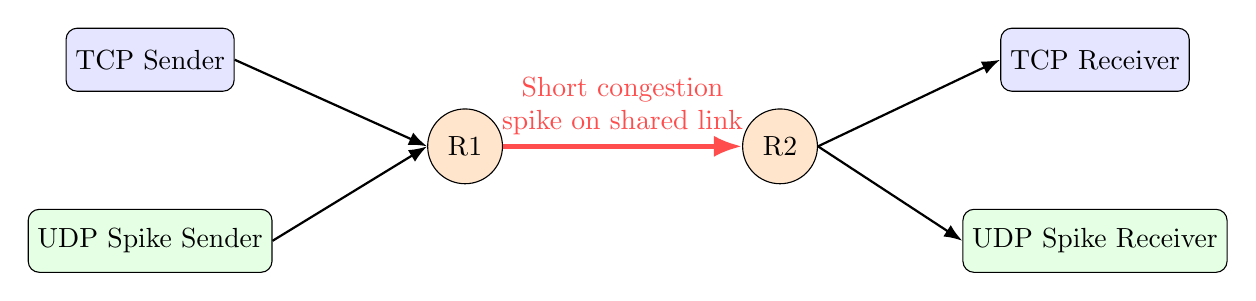
\begin{tikzpicture}[
    host/.style={draw, rounded corners, minimum width=1.8cm, minimum height=0.8cm, fill=blue!10},
    spike/.style={draw, rounded corners, minimum width=2.0cm, minimum height=0.8cm, fill=green!10},
    router/.style={draw, circle, minimum size=0.95cm, fill=orange!20},
    link/.style={-Latex, thick},
    bottleneck/.style={-Latex, ultra thick, red!70}
  ]
    \node[host] (tcpS) at (0,1.3) {TCP Sender};
    \node[spike] (udpS) at (0,-1.0) {UDP Spike Sender};
    \node[router] (r1) at (4,0.2) {R1};
    \node[router] (r2) at (8,0.2) {R2};
    \node[host] (tcpR) at (12,1.3) {TCP Receiver};
    \node[spike] (udpR) at (12,-1.0) {UDP Spike Receiver};

    \draw[link] (tcpS.east) -- (r1.west);
    \draw[link] (udpS.east) -- (r1.west);
    \draw[bottleneck] (r1) -- node[above, align=center] {Short congestion\\spike on shared link} (r2);
    \draw[link] (r2.east) -- (tcpR.west);
    \draw[link] (r2.east) -- (udpR.west);
  \end{tikzpicture}

  \vspace{0.4cm}
  \begin{itemize}
    \item One continuous TCP flow is observed.
    \item A short UDP burst is injected to create a temporary RTT spike.
    \item This isolates the main EL-RTO idea: suppress overreaction to brief congestion.
  \end{itemize}
\end{frame}

\begin{frame}{Checklist Wireless Experiment Driver}
  \textbf{File:} \texttt{scratch/rto-checklist-wireless.cc}

  \begin{itemize}
    \item Single experiment driver for both assigned wireless networks.
    \item Supports command-line control of:
    \begin{itemize}
      \item network type
      \item RTO mode
      \item nodes
      \item flows
      \item packets per second
      \item speed
      \item simulation time
    \end{itemize}
    \item Produces one result row per run:
    \begin{itemize}
      \item throughput
      \item average delay
      \item packet delivery ratio
      \item drop ratio
      \item energy
    \end{itemize}
  \end{itemize}
\end{frame}

\begin{frame}{Wireless 802.11 Mobile Topology}
  \centering
  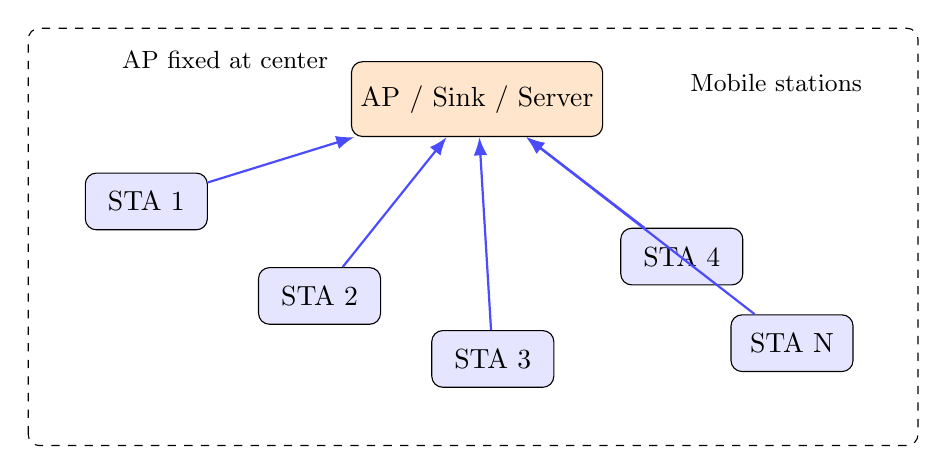
\begin{tikzpicture}[
    ap/.style={draw, rounded corners, minimum width=2.1cm, minimum height=0.95cm, fill=orange!20},
    sta/.style={draw, rounded corners, minimum width=1.55cm, minimum height=0.72cm, fill=blue!10},
    flow/.style={-Latex, thick, blue!70}
  ]
    \draw[dashed, rounded corners] (-0.5,-2.3) rectangle (10.8,3.0);
    \node[ap] (ap) at (5.2,2.1) {AP / Sink / Server};

    \node[sta] (s1) at (1.0,0.8) {STA 1};
    \node[sta] (s2) at (3.2,-0.4) {STA 2};
    \node[sta] (s3) at (5.4,-1.2) {STA 3};
    \node[sta] (s4) at (7.8,0.1) {STA 4};
    \node[sta] (sn) at (9.2,-1.0) {STA N};

    \draw[flow] (s1) -- (ap);
    \draw[flow] (s2) -- (ap);
    \draw[flow] (s3) -- (ap);
    \draw[flow] (s4) -- (ap);
    \draw[flow] (sn) -- (ap);

    \node[align=left] at (9.0,2.3) {\small Mobile stations};
    \node[align=left] at (2.0,2.6) {\small AP fixed at center};
  \end{tikzpicture}

  \vspace{0.3cm}
  \begin{itemize}
    \item Node 0 acts as the AP, sink, and TCP server.
    \item Remaining nodes are mobile stations using Random Waypoint mobility.
    \item Traffic direction: stations send TCP flows toward the AP sink.
  \end{itemize}
\end{frame}

\begin{frame}{Why the Wi-Fi Scenario Was Reworked}
  \begin{itemize}
    \item The earlier Wi-Fi setup produced repeated zero-throughput behavior.
    \item The final working design uses:
    \begin{itemize}
      \item infrastructure Wi-Fi
      \item one AP and multiple STA nodes
      \item fixed-rate \texttt{802.11b}
      \item \texttt{NonUnicastMode = DsssRate11Mbps}
    \end{itemize}
    \item Reason for this simplification:
    \begin{itemize}
      \item more stable association and data exchange
      \item reliable ARP and control-frame handling
      \item repeatable checklist results on limited hardware
    \end{itemize}
    \item Wi-Fi energy was measured using:
    \begin{itemize}
      \item \texttt{BasicEnergySourceHelper}
      \item \texttt{WifiRadioEnergyModelHelper}
    \end{itemize}
  \end{itemize}
\end{frame}

\begin{frame}{Wireless 802.15.4 Mobile Topology}
  \centering
  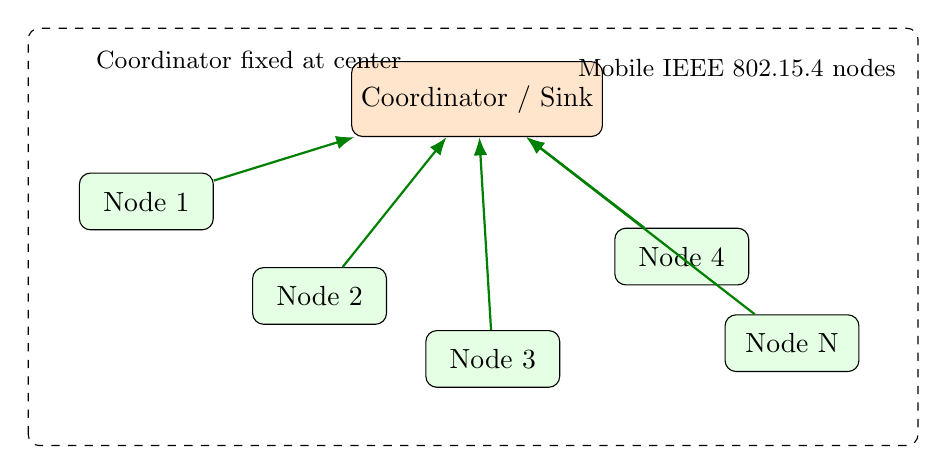
\begin{tikzpicture}[
    coord/.style={draw, rounded corners, minimum width=2.3cm, minimum height=0.95cm, fill=orange!20},
    nodebox/.style={draw, rounded corners, minimum width=1.7cm, minimum height=0.72cm, fill=green!10},
    flow/.style={-Latex, thick, green!50!black}
  ]
    \draw[dashed, rounded corners] (-0.5,-2.3) rectangle (10.8,3.0);
    \node[coord] (c) at (5.2,2.1) {Coordinator / Sink};

    \node[nodebox] (n1) at (1.0,0.8) {Node 1};
    \node[nodebox] (n2) at (3.2,-0.4) {Node 2};
    \node[nodebox] (n3) at (5.4,-1.2) {Node 3};
    \node[nodebox] (n4) at (7.8,0.1) {Node 4};
    \node[nodebox] (nn) at (9.2,-1.0) {Node N};

    \draw[flow] (n1) -- (c);
    \draw[flow] (n2) -- (c);
    \draw[flow] (n3) -- (c);
    \draw[flow] (n4) -- (c);
    \draw[flow] (nn) -- (c);

    \node[align=left] at (8.5,2.5) {\small Mobile IEEE 802.15.4 nodes};
    \node[align=left] at (2.3,2.6) {\small Coordinator fixed at center};
  \end{tikzpicture}

  \vspace{0.25cm}
  \begin{itemize}
    \item Node 0 is the fixed coordinator and sink.
    \item Remaining nodes are mobile LR-WPAN devices.
    \item Protocol stack:
    \[
      802.15.4 \rightarrow 6LoWPAN \rightarrow IPv6 \rightarrow TCP
    \]
  \end{itemize}
\end{frame}

\begin{frame}{Why a Custom LR-WPAN Energy Tracker Was Added}
  \begin{itemize}
    \item Wi-Fi and LR-WPAN do not expose energy accounting in the same way.
    \item For LR-WPAN, a custom \texttt{LrWpanEnergyTracker} was added.
    \item It listens to PHY \texttt{TrxState} transitions and integrates:
    \[
      Energy = Current \times Voltage \times Time
    \]
    \item This made it possible to report total checklist energy consumption for:
    \begin{itemize}
      \item transmission
      \item reception
      \item idle/off periods
    \end{itemize}
  \end{itemize}
\end{frame}

\begin{frame}{Checklist Parameter Sweeps}
  \begin{itemize}
    \item For both assigned mobile networks, the following were varied:
    \begin{itemize}
      \item node count: 20, 40, 60, 80, 100
      \item flow count: 10, 20, 30, 40, 50
      \item packet rate: 100, 200, 300, 400, 500 pps
      \item node speed: 5, 10, 15, 20, 25 m/s
    \end{itemize}
    \item Area-scale sweep was intentionally not used.
    \item Reason:
    \begin{itemize}
      \item the checklist requires area variation for static-node cases
      \item the assigned cases are mobile-only
    \end{itemize}
  \end{itemize}
\end{frame}

\begin{frame}{Metrics Collected}
  \begin{itemize}
    \item Throughput
    \item End-to-end delay
    \item Packet delivery ratio
    \item Drop ratio
    \item Energy consumption
  \end{itemize}

  \vspace{0.3cm}
  \textbf{How they were measured}
  \begin{itemize}
    \item FlowMonitor for packet, byte, and delay statistics
    \item Wi-Fi energy model for 802.11 scenarios
    \item Custom PHY-state tracker for LR-WPAN scenarios
    \item One CSV result row per experiment run
  \end{itemize}
\end{frame}

\begin{frame}{Why Helper Scripts Were Added}
  \begin{itemize}
    \item The full wireless matrix was too heavy to run reliably in one shot on the laptop.
    \item Added resumable experiment runner:
    \begin{itemize}
      \item \texttt{run-selected-checklist.py}
    \end{itemize}
    \item Added single-network wrappers:
    \begin{itemize}
      \item \texttt{run-wifi-mobile-10s.py}
      \item \texttt{run-lrwpan-mobile-10s.py}
    \end{itemize}
    \item Added plot automation:
    \begin{itemize}
      \item \texttt{plot-checklist-wireless.py}
    \end{itemize}
    \item These scripts made the workflow:
    \begin{itemize}
      \item repeatable
      \item resumable
      \item easier to verify
    \end{itemize}
  \end{itemize}
\end{frame}

\begin{frame}{Practical Engineering Decisions}
  \begin{itemize}
    \item Checklist runs used \texttt{simTime = 10s} instead of 20s.
    \item Reason:
    \begin{itemize}
      \item large Wi-Fi cases were too slow for the available machine
      \item 10 seconds preserved the sweep structure while making the experiments feasible
    \end{itemize}
    \item Plotting was updated so that overlapping \texttt{Improved} and \texttt{EL-RTO} curves are clearly indicated.
    \item This matters because, in some wireless sweeps, those two modes produced identical results.
  \end{itemize}
\end{frame}

\section{Results}
\begin{frame}{Base Paper Replication Results}
  \begin{columns}[T]
    \column{0.5\textwidth}
    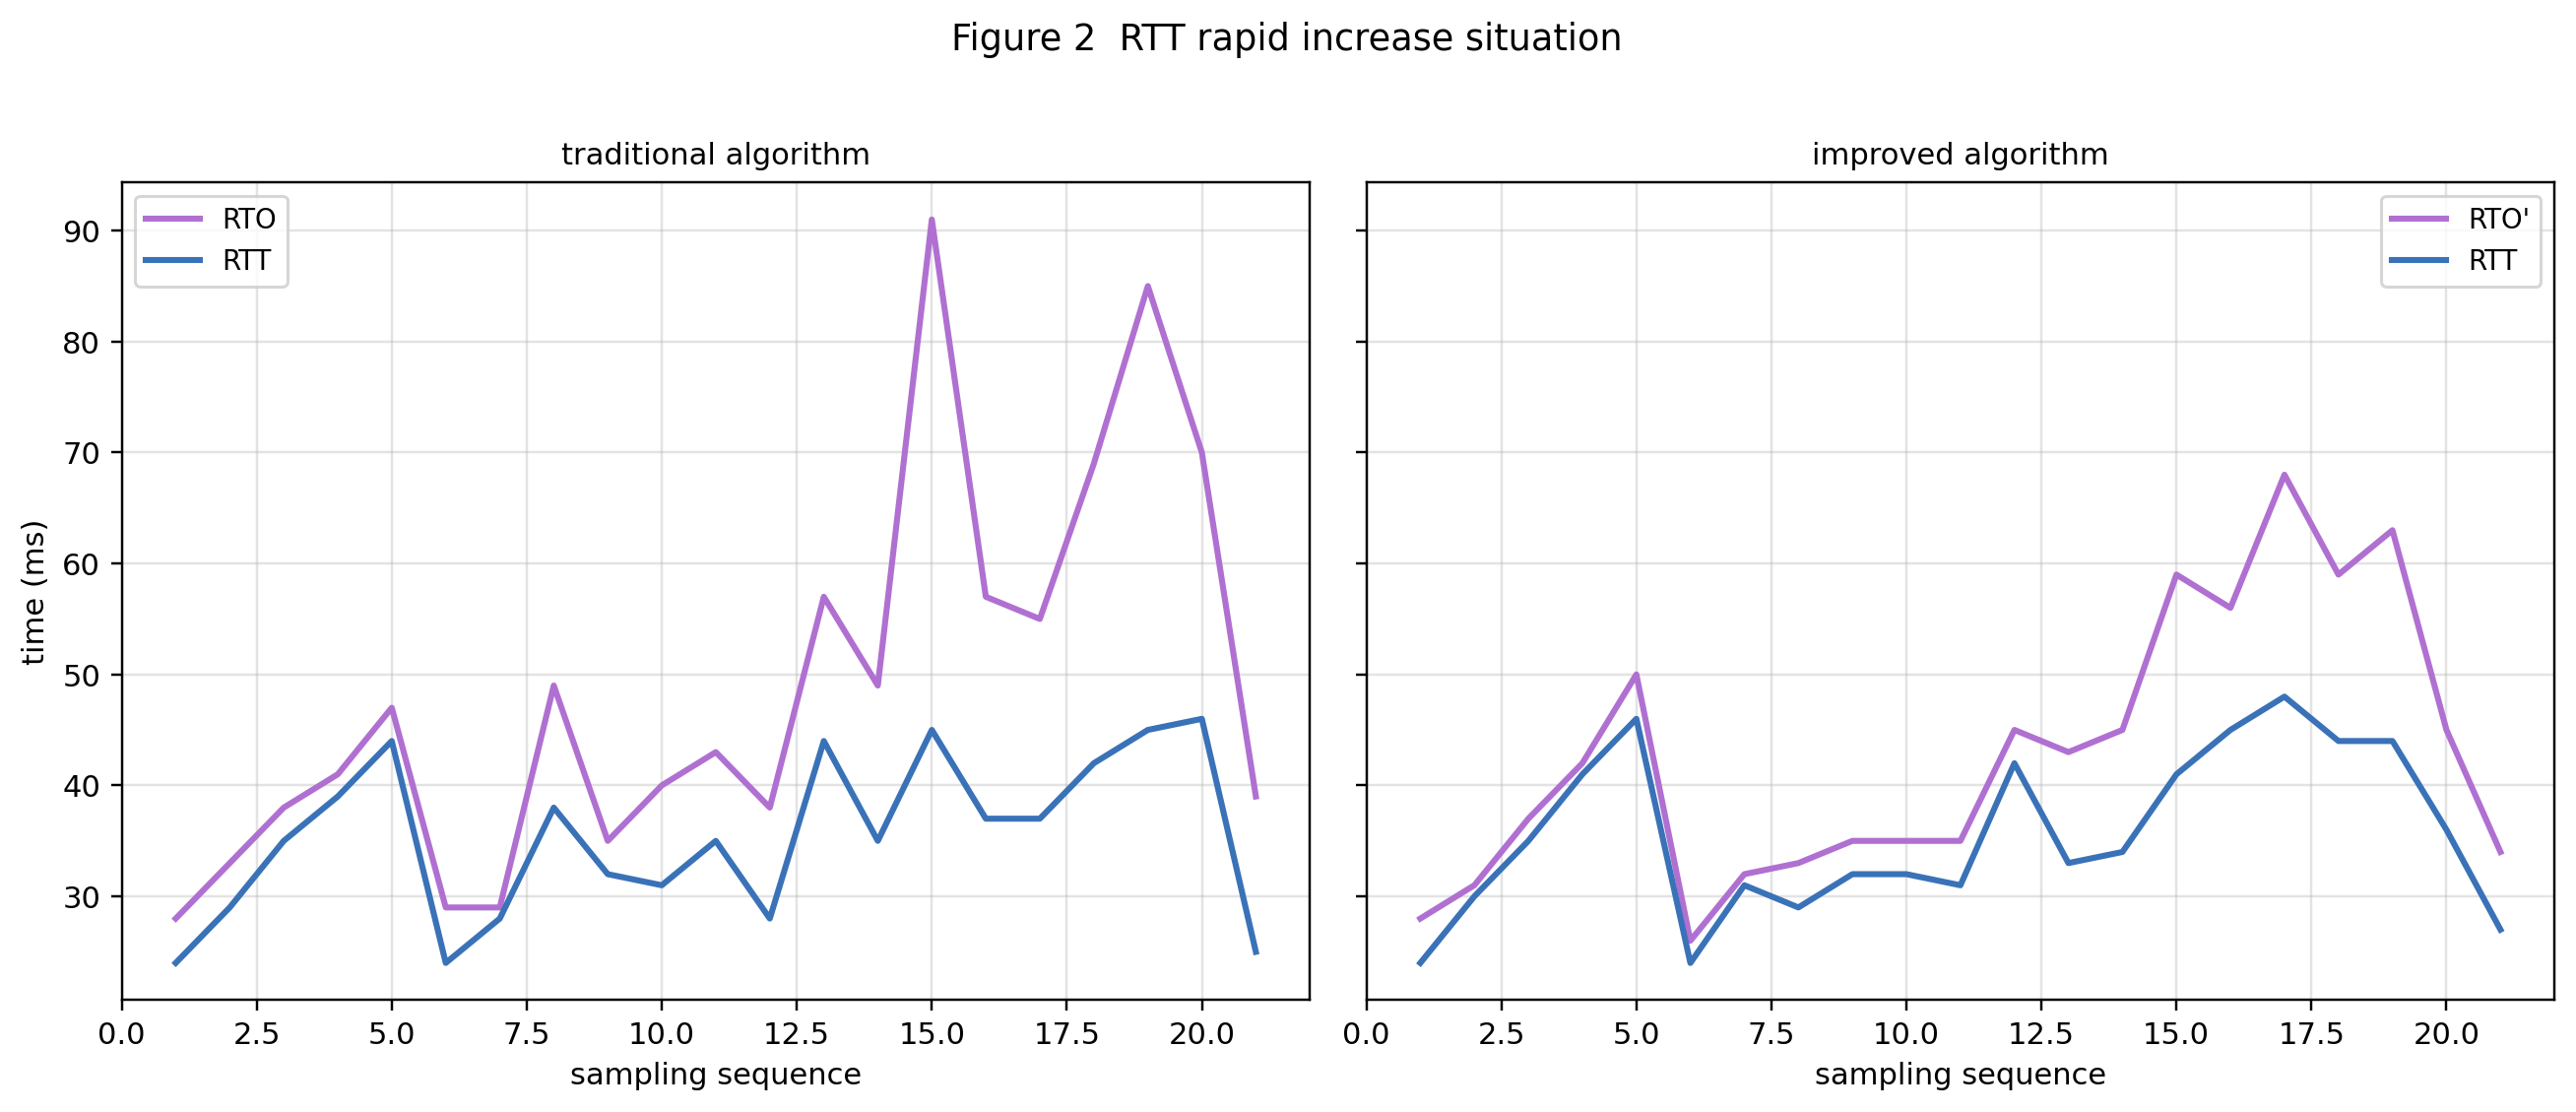
\includegraphics[width=\linewidth]{2105114_final_submission/base_paper_results/figure2_increase.png}

    \column{0.5\textwidth}
    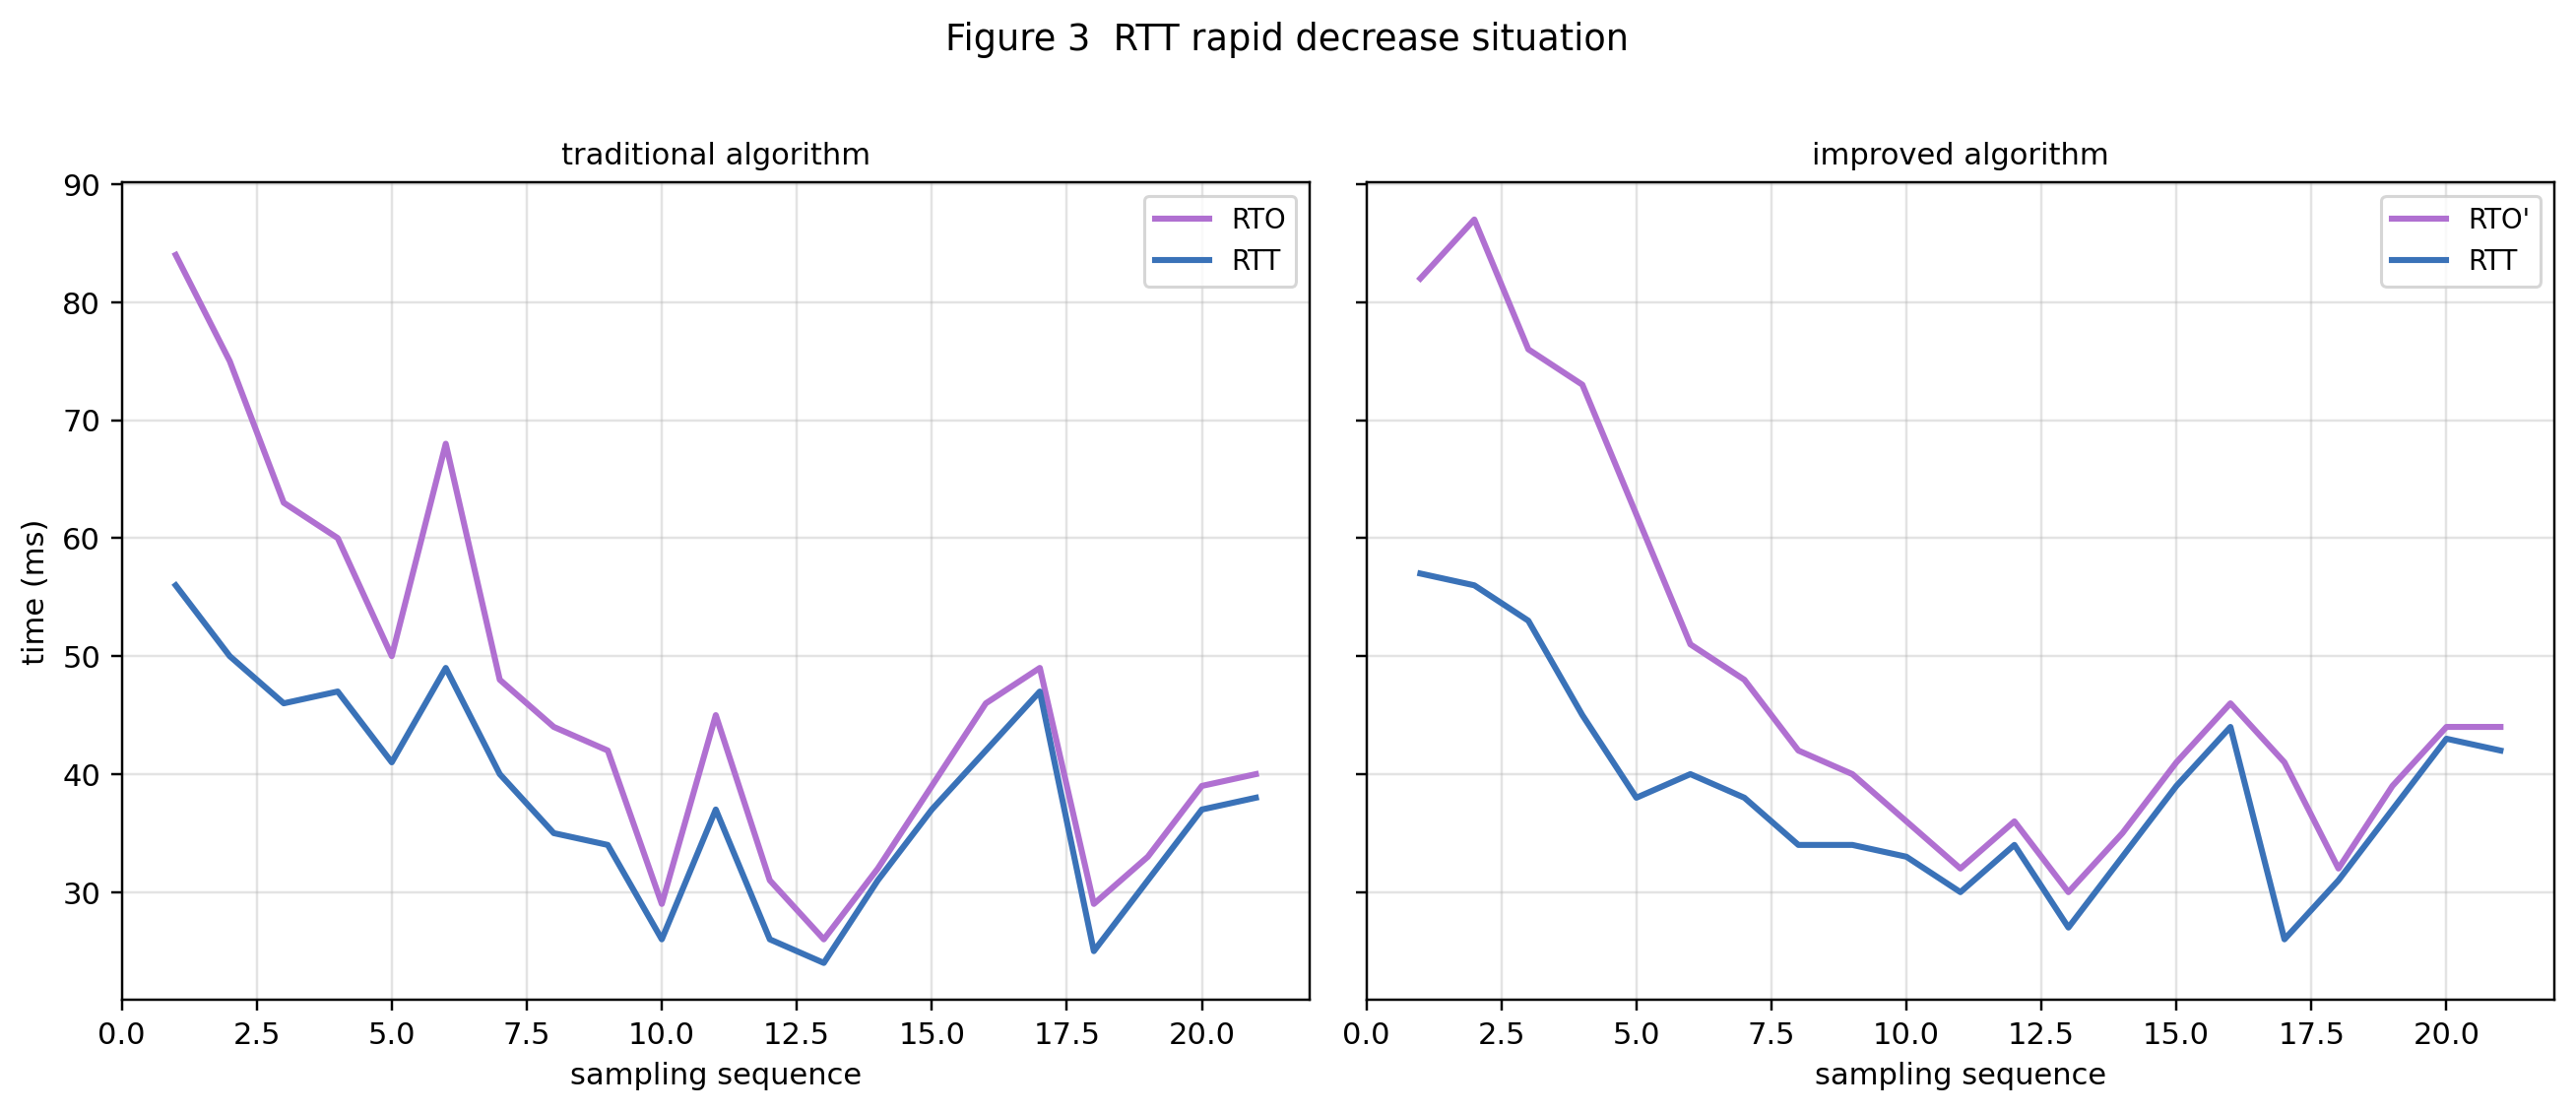
\includegraphics[width=\linewidth]{2105114_final_submission/base_paper_results/figure3_decrease.png}
  \end{columns}

  \vspace{0.3cm}
  \begin{itemize}
    \item Increase-case average gamma: Standard 35.10, Improved 19.14
    \item Decrease-case average gamma: Standard 19.56, Improved 23.09
    \item Throughput remained close in both cases: around 11 Mbps
  \end{itemize}
\end{frame}

\begin{frame}{EL-RTO Spike Experiment Results}
  \begin{columns}[T]
    \column{0.5\textwidth}
    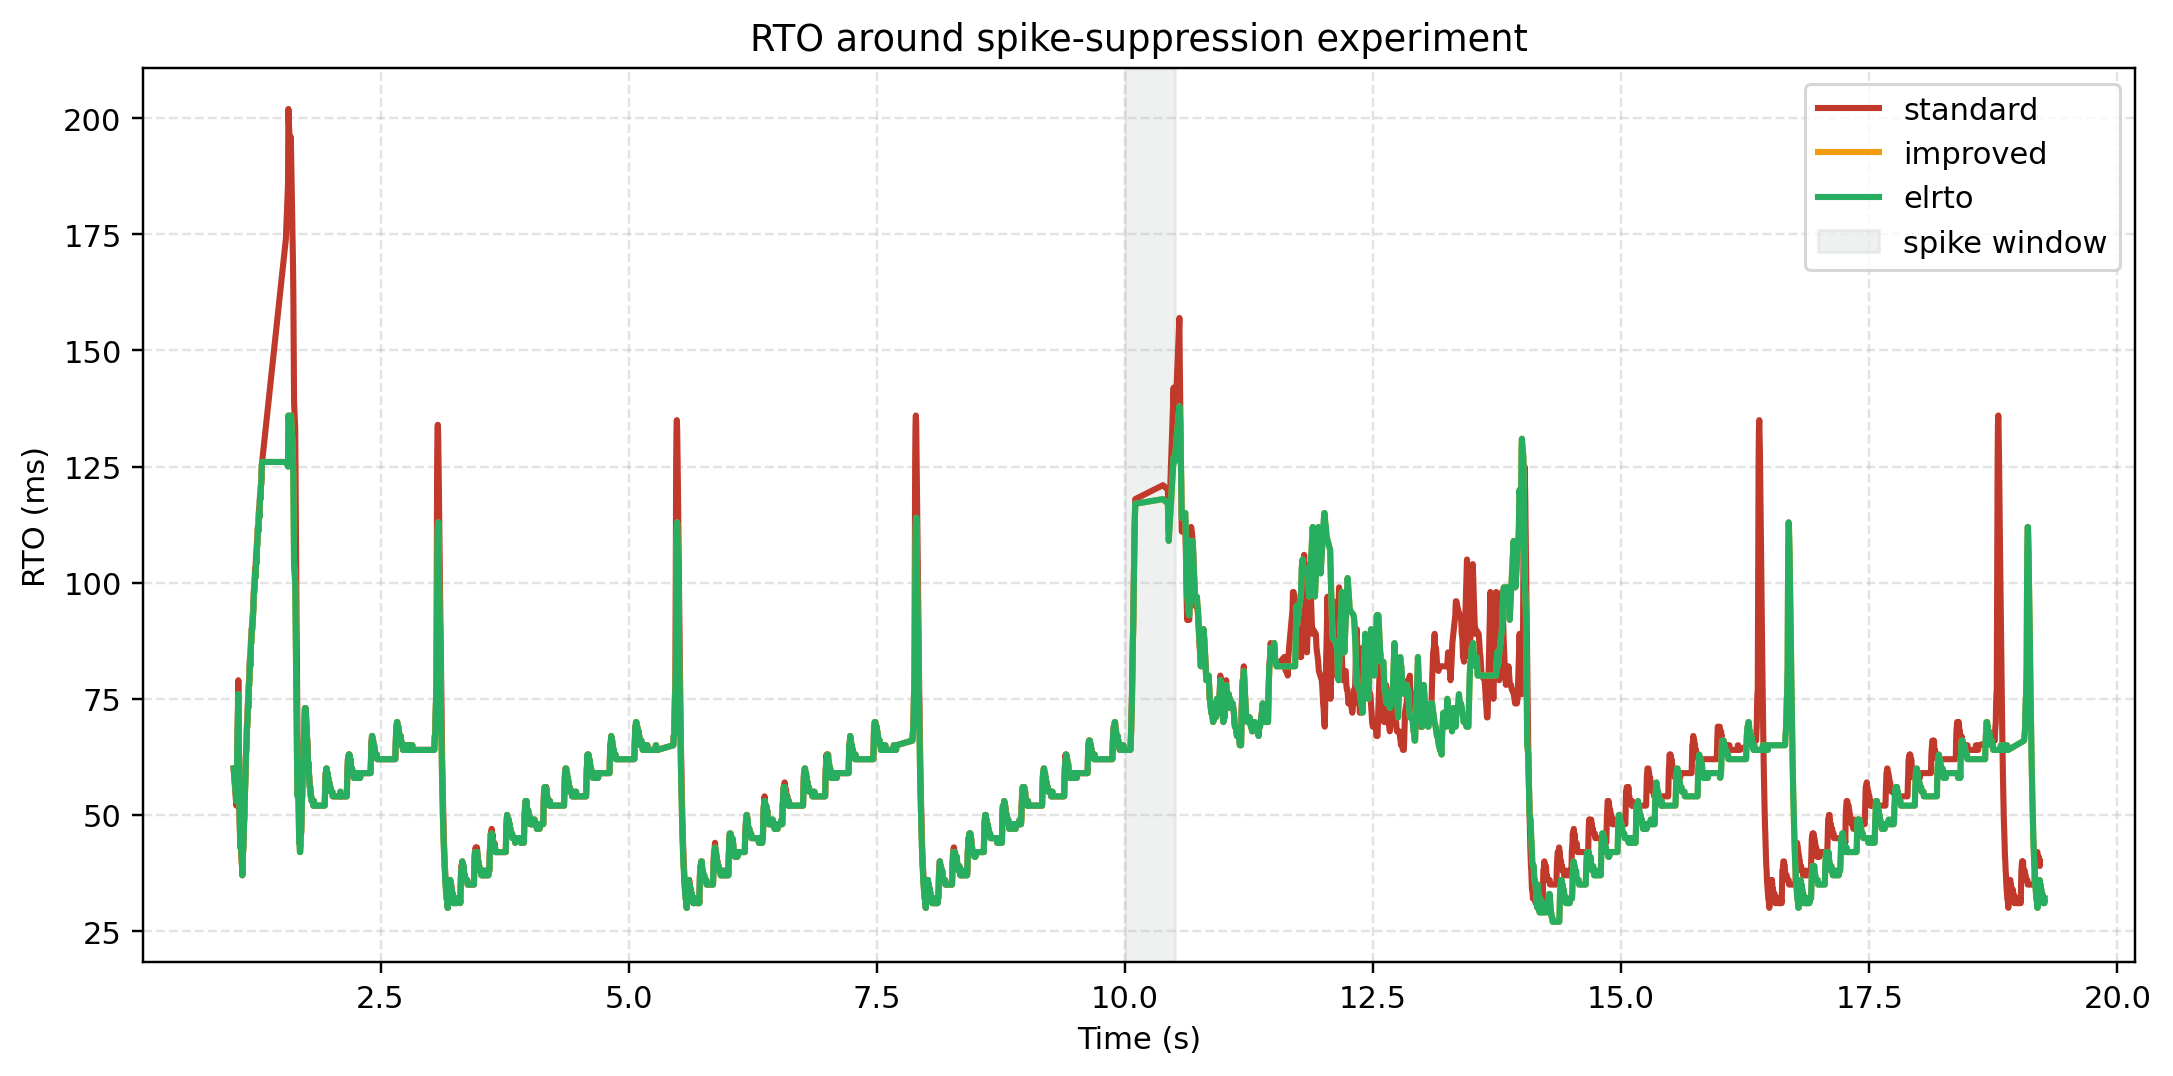
\includegraphics[width=\linewidth]{2105114_final_submission/base_paper_elrto_artifacts/elrto_spike_rto.png}

    \column{0.5\textwidth}
    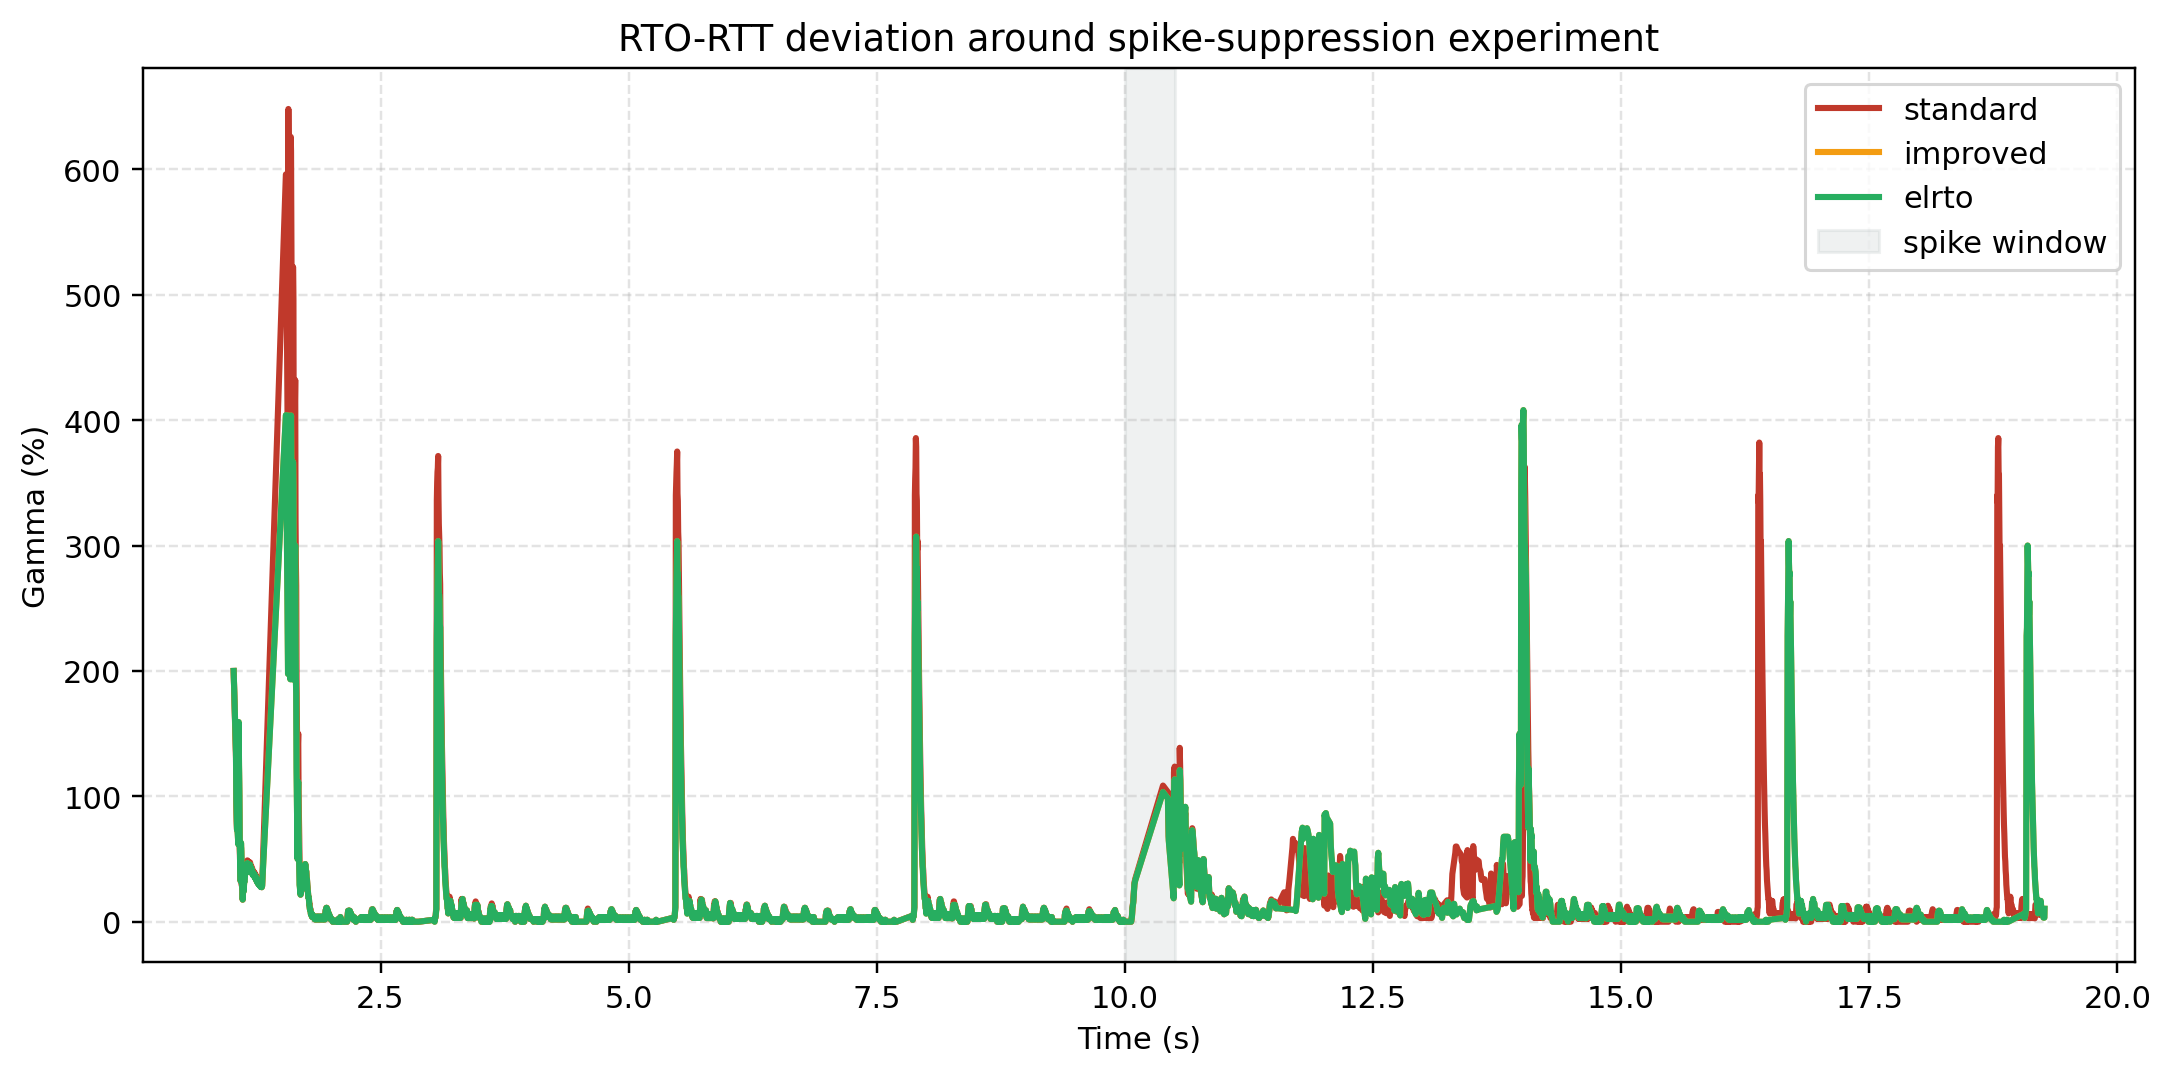
\includegraphics[width=\linewidth]{2105114_final_submission/base_paper_elrto_artifacts/elrto_spike_gamma.png}
  \end{columns}

  \vspace{0.2cm}
  \footnotesize
  \begin{tabular}{lccc}
    \toprule
    Mode & Peak RTO & Avg Gap & Avg Gamma \\
    \midrule
    Standard & 142 & 13.034 & 19.073 \\
    Improved & 127 & 11.759 & 17.410 \\
    EL-RTO & 127 & 11.759 & 17.410 \\
    \bottomrule
  \end{tabular}

  \vspace{0.2cm}
  \begin{itemize}
    \item Standard mode inflated RTO more during the induced spike.
    \item Improved and EL-RTO reduced the RTO-RTT mismatch in this scenario.
  \end{itemize}
\end{frame}

\begin{frame}{Wi-Fi Mobile: Throughput and Delay}
  \begin{columns}[T]
    \column{0.5\textwidth}
    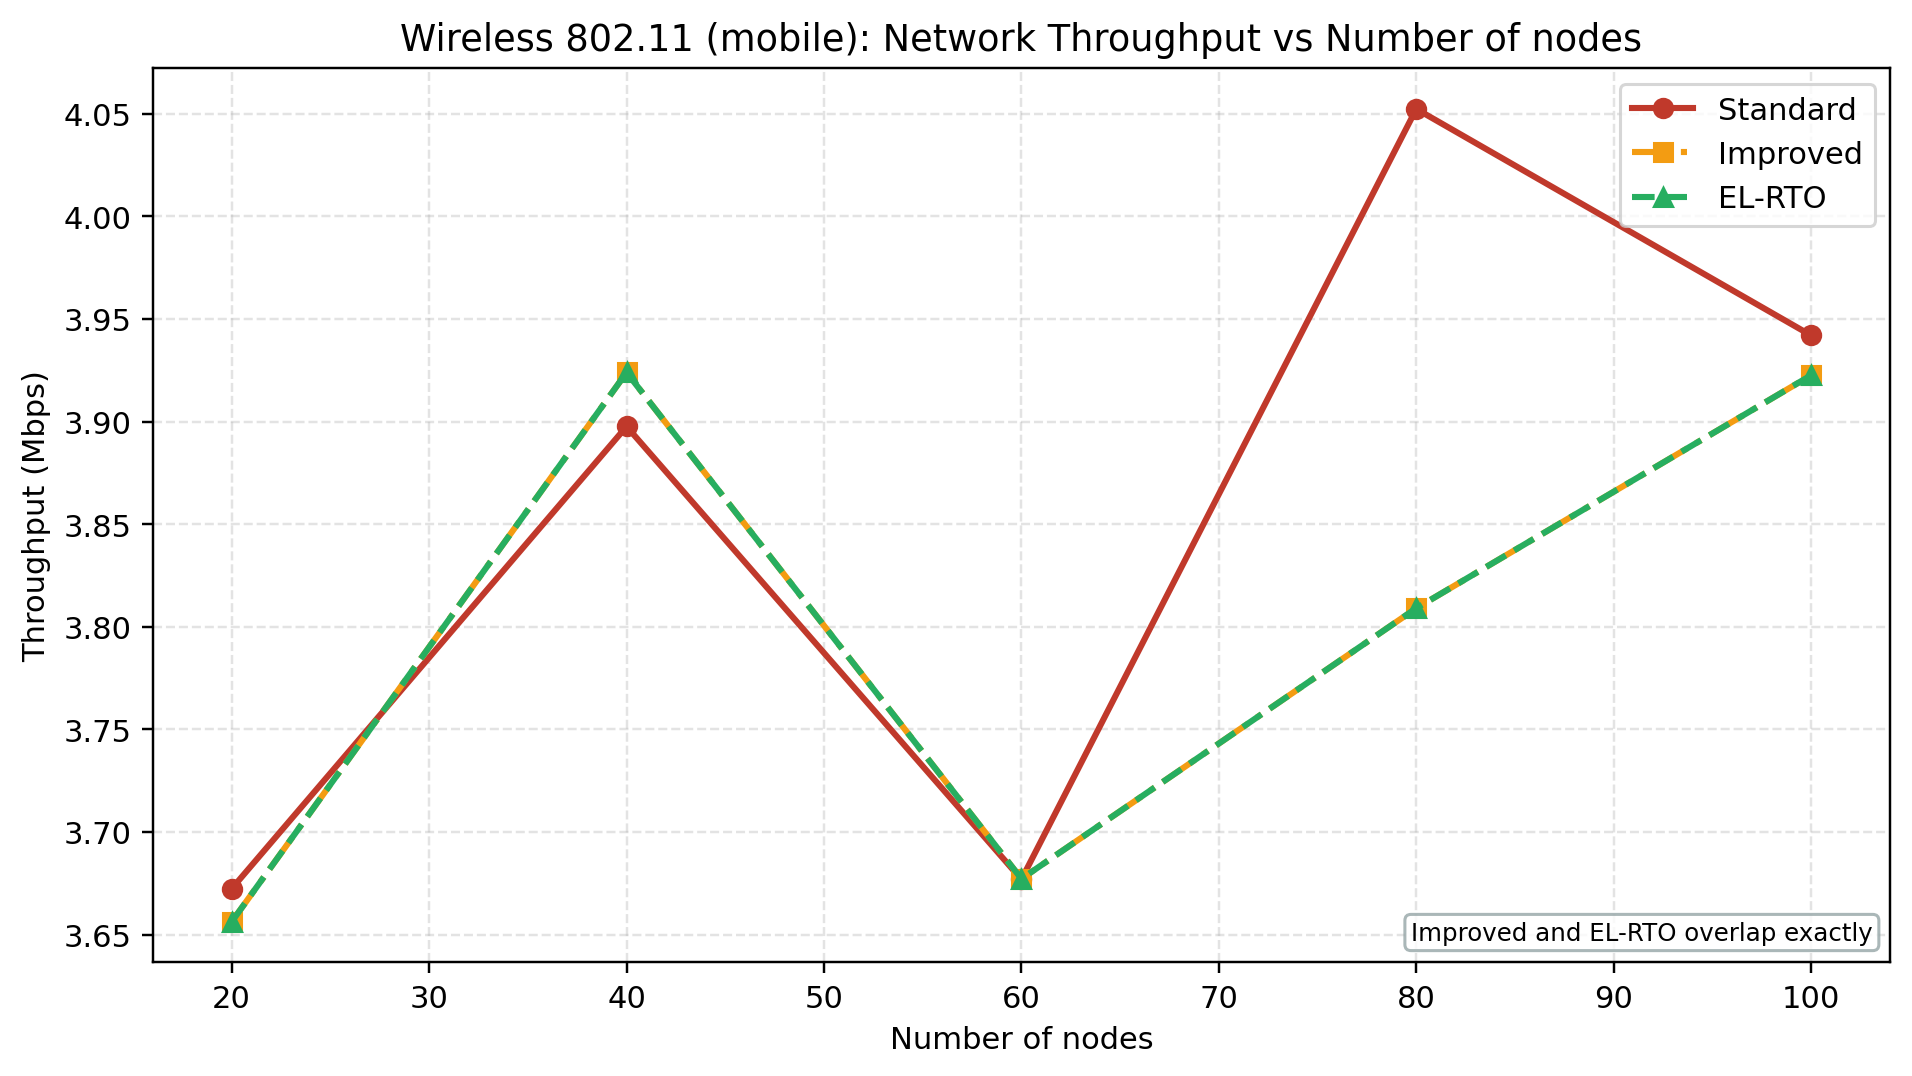
\includegraphics[width=\linewidth]{2105114_final_submission/wifi_mobile/student2105114_wifi_mobile_10s_plots/wifi-mobile_nodes_throughputMbps.png}

    \column{0.5\textwidth}
    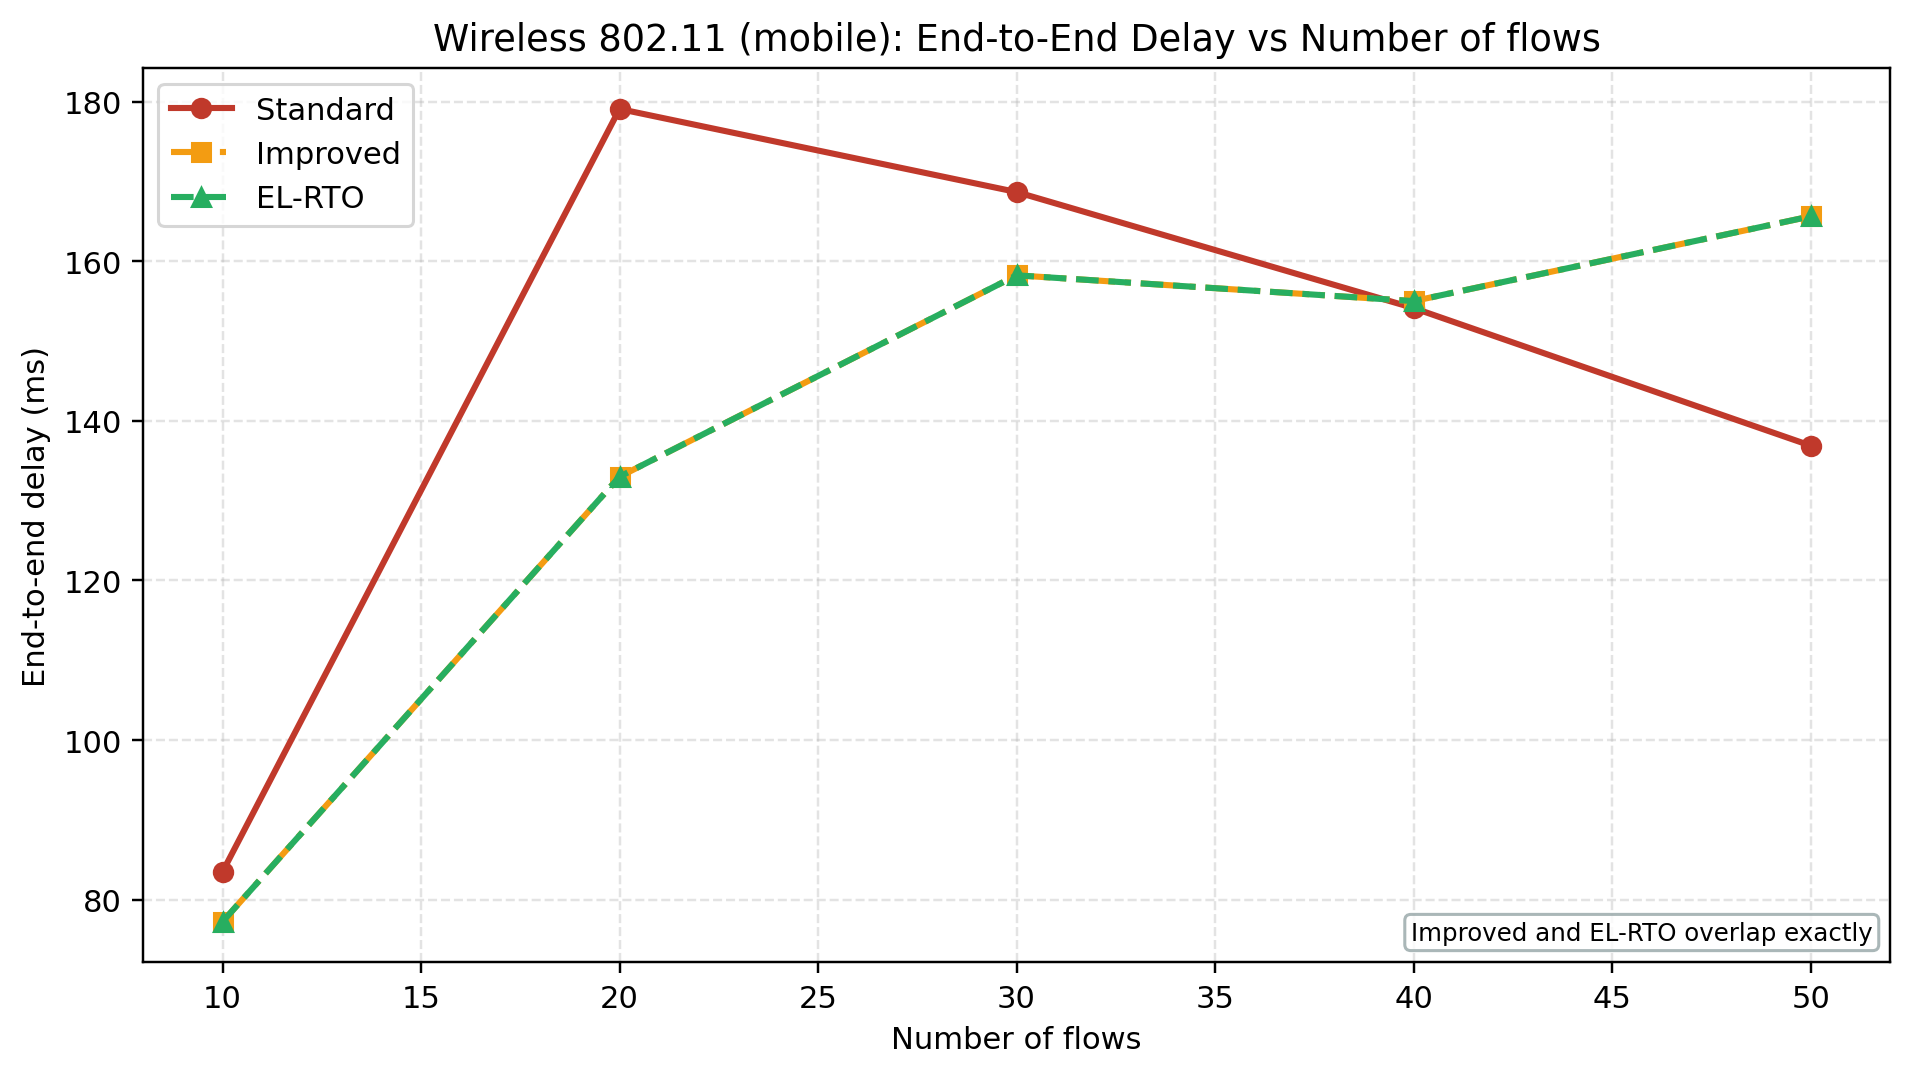
\includegraphics[width=\linewidth]{2105114_final_submission/wifi_mobile/student2105114_wifi_mobile_10s_plots/wifi-mobile_flows_averageDelayMs.png}
  \end{columns}

  \vspace{0.2cm}
  \footnotesize
  \begin{tabular}{lccc}
    \toprule
    Sweep & Mode & Avg Throughput & Avg Delay \\
    \midrule
    Nodes & Standard & 3.848 & 73.936 \\
    Nodes & Improved & 3.798 & 71.562 \\
    Flows & Standard & 4.181 & 144.445 \\
    Flows & Improved & 4.169 & 137.815 \\
    \bottomrule
  \end{tabular}

  \vspace{0.2cm}
  \begin{itemize}
    \item Wi-Fi delivered the highest throughput among the assigned networks.
    \item Improved and EL-RTO overlap in these Wi-Fi checklist plots because the measured values are identical.
  \end{itemize}
\end{frame}

\begin{frame}{Wi-Fi Mobile: Reliability and Energy}
  \begin{columns}[T]
    \column{0.5\textwidth}
    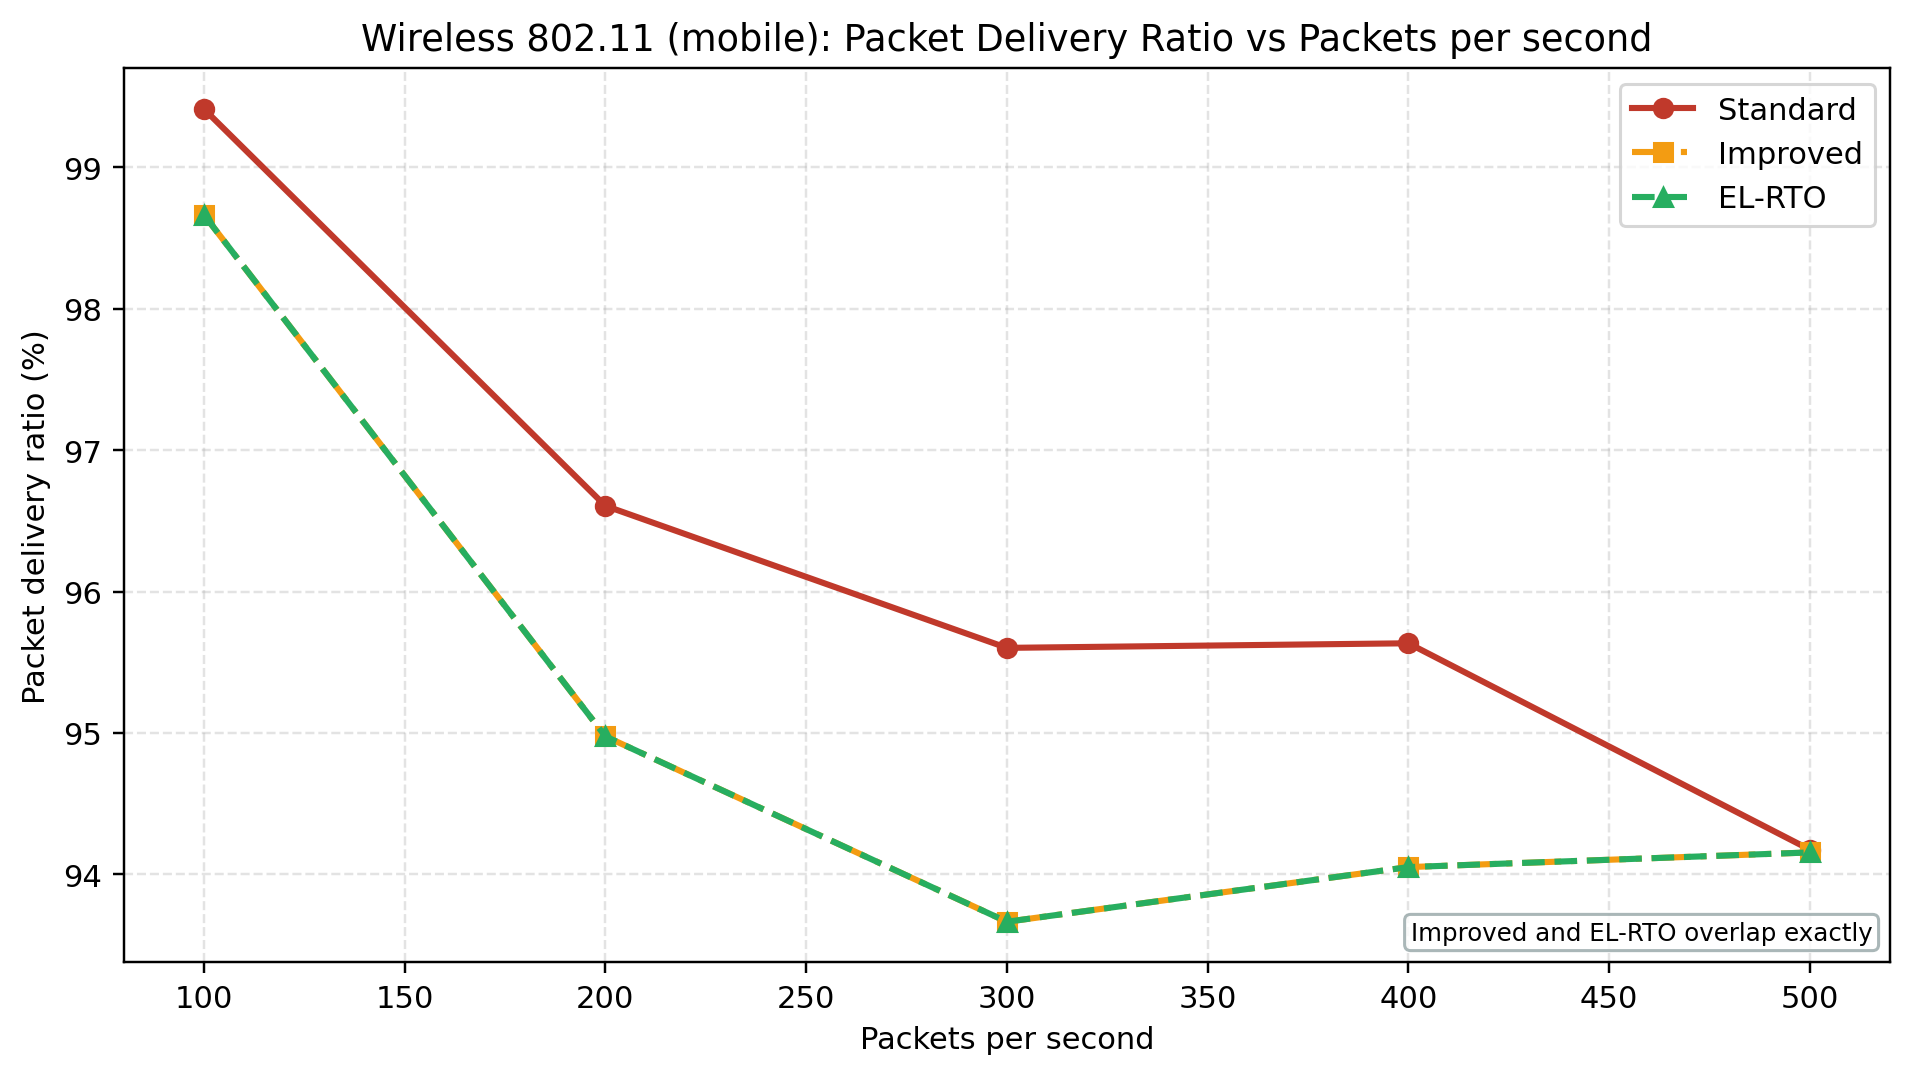
\includegraphics[width=\linewidth]{2105114_final_submission/wifi_mobile/student2105114_wifi_mobile_10s_plots/wifi-mobile_pps_pdrPct.png}

    \column{0.5\textwidth}
    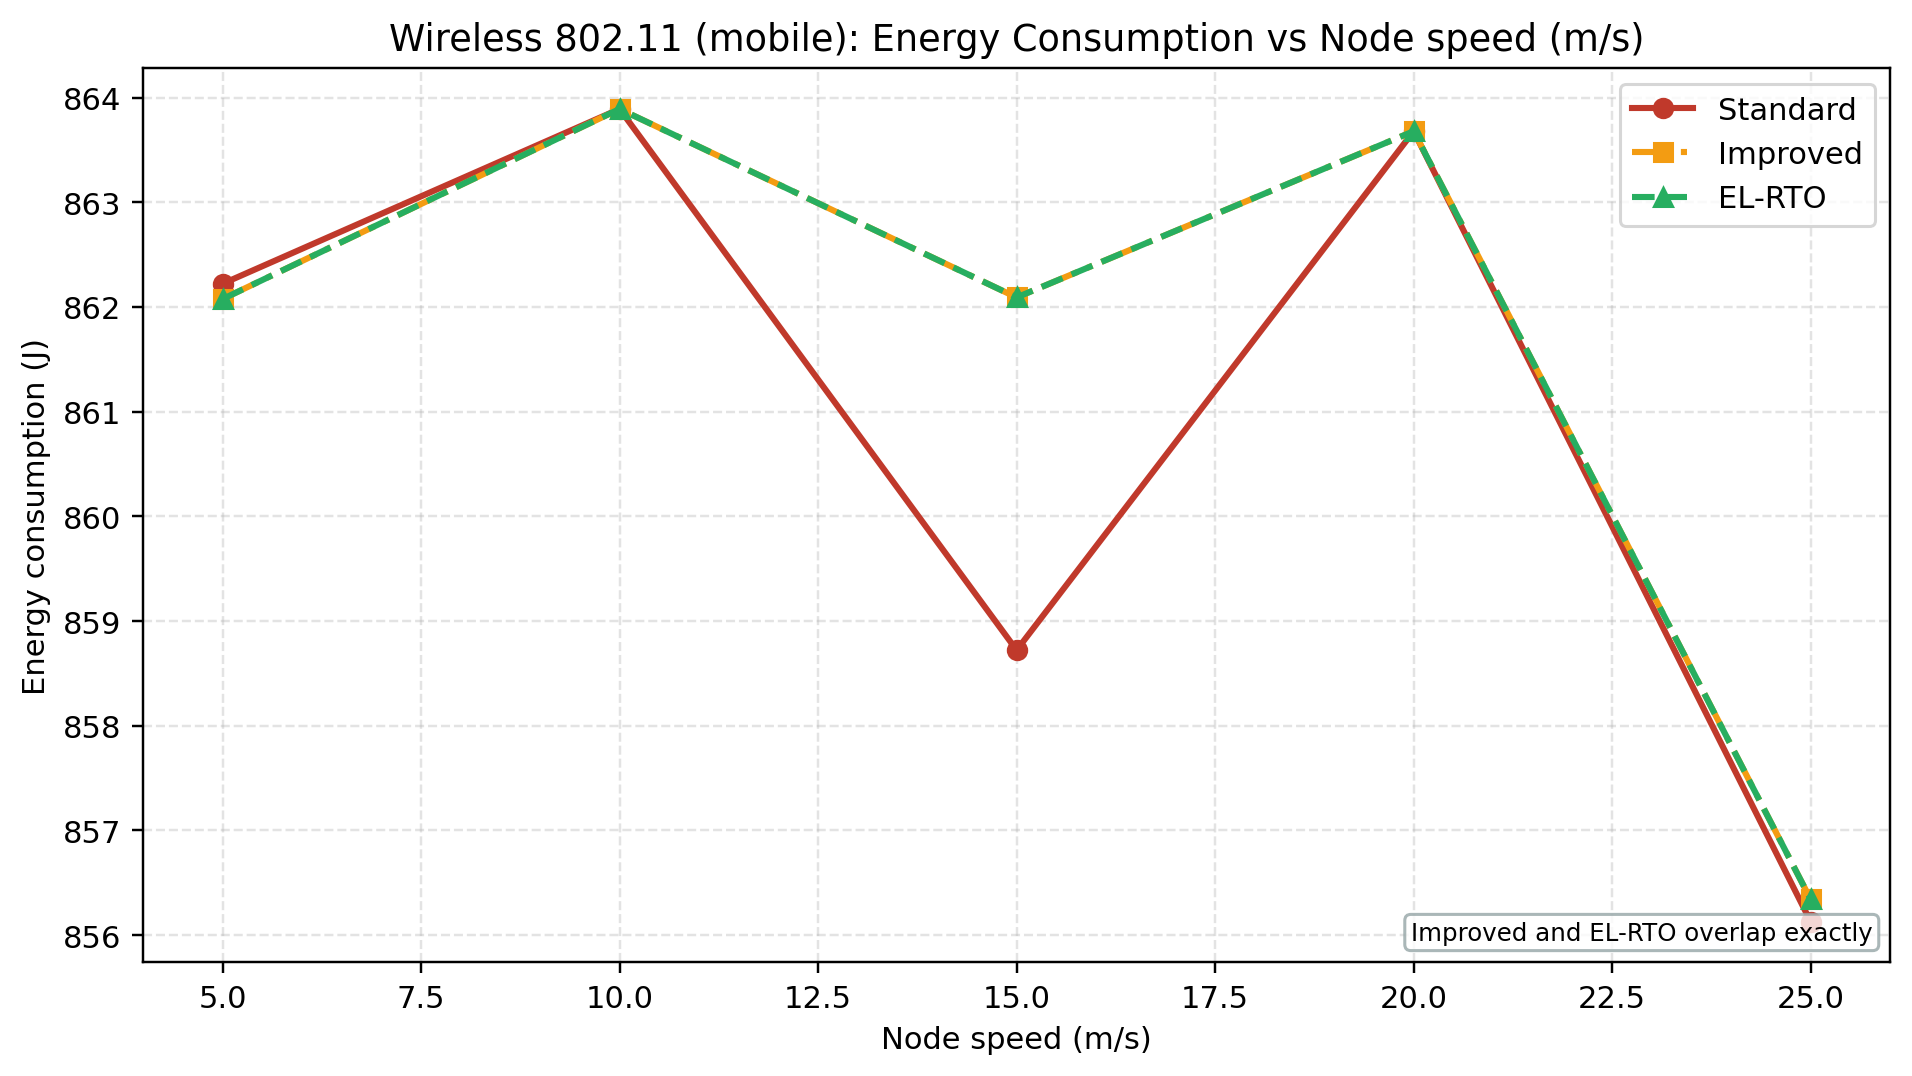
\includegraphics[width=\linewidth]{2105114_final_submission/wifi_mobile/student2105114_wifi_mobile_10s_plots/wifi-mobile_speed_energyJ.png}
  \end{columns}

  \vspace{0.2cm}
  \footnotesize
  \begin{tabular}{lccc}
    \toprule
    Sweep & Mode & Avg PDR (\%) & Avg Energy (J) \\
    \midrule
    Nodes & Standard & 99.145 & 517.511 \\
    Nodes & Improved & 99.223 & 517.270 \\
    Speed & Standard & 98.514 & 860.928 \\
    Speed & Improved & 98.201 & 861.615 \\
    \bottomrule
  \end{tabular}
\end{frame}

\begin{frame}{LR-WPAN Mobile: Throughput and Delay}
  \begin{columns}[T]
    \column{0.5\textwidth}
    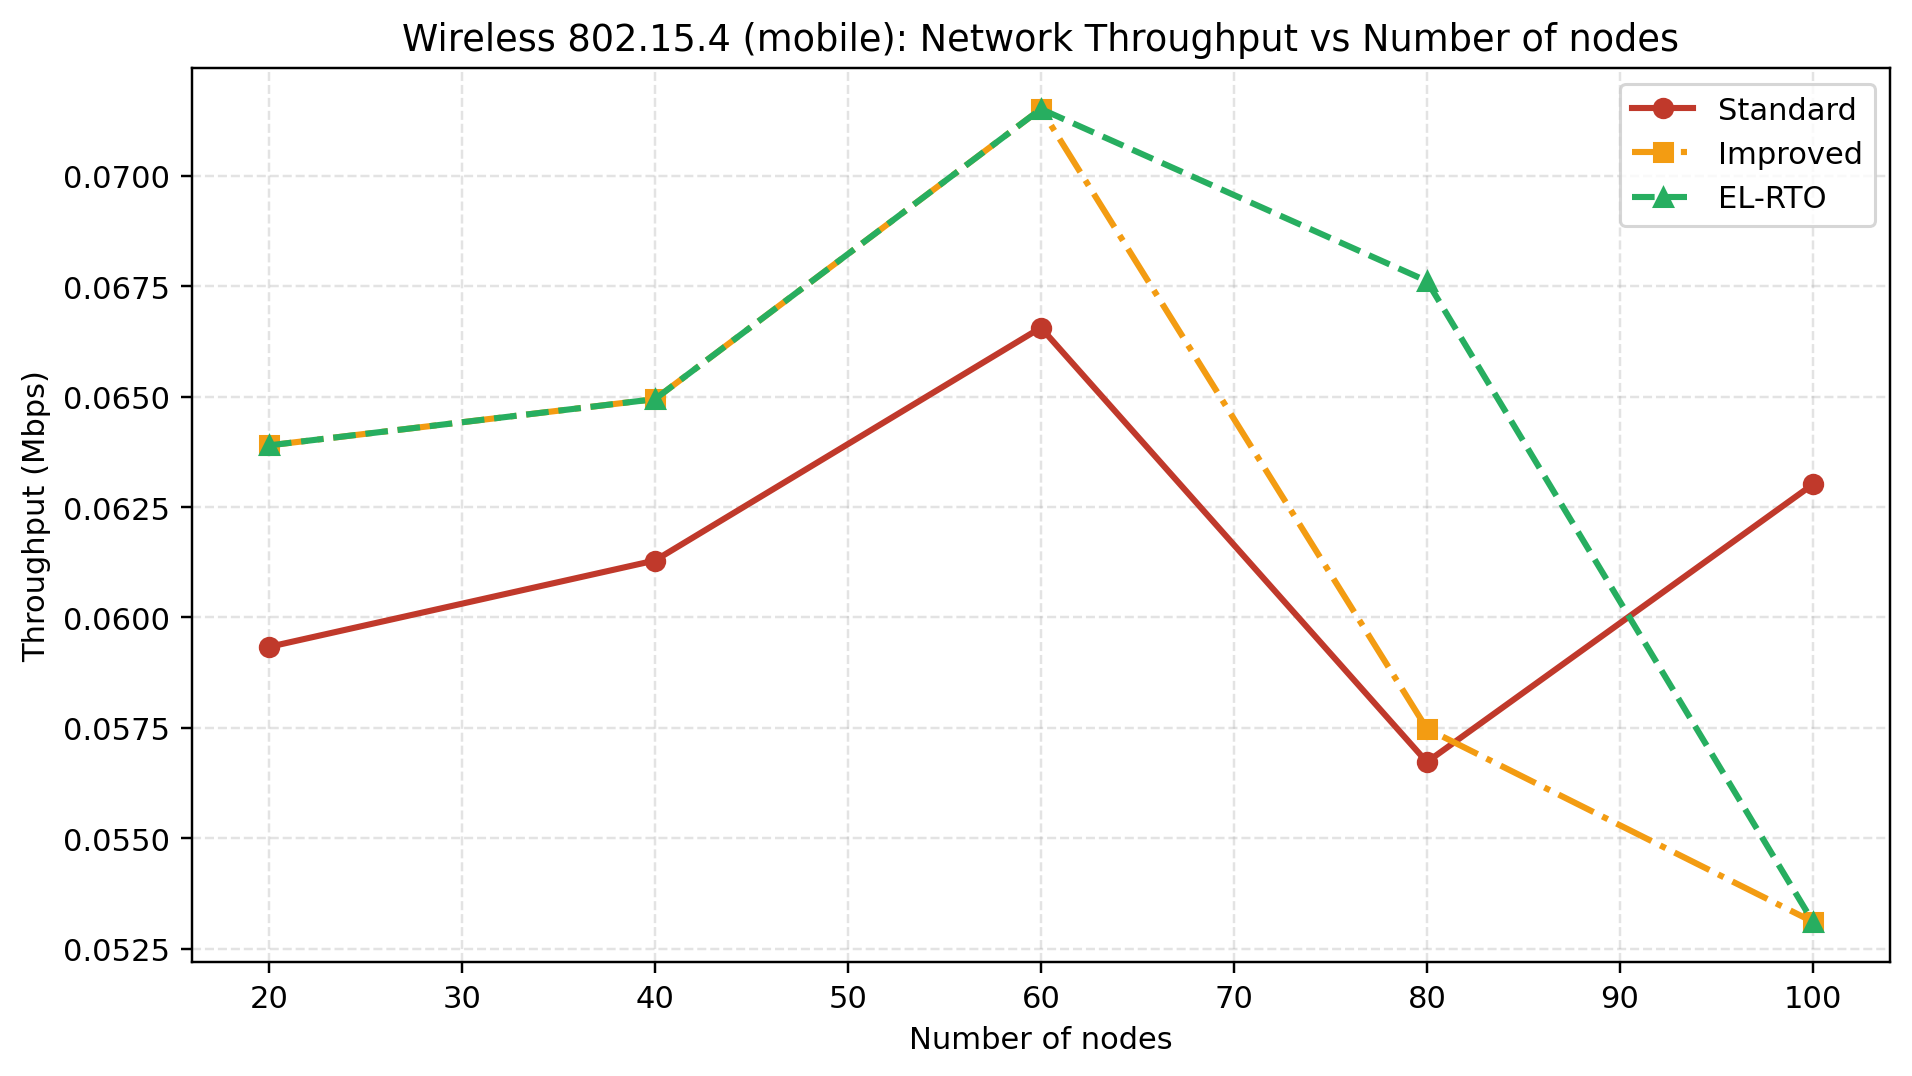
\includegraphics[width=\linewidth]{2105114_final_submission/lrwpan_mobile/student2105114_lrwpan_mobile_10s_plots/lrwpan-mobile_nodes_throughputMbps.png}

    \column{0.5\textwidth}
    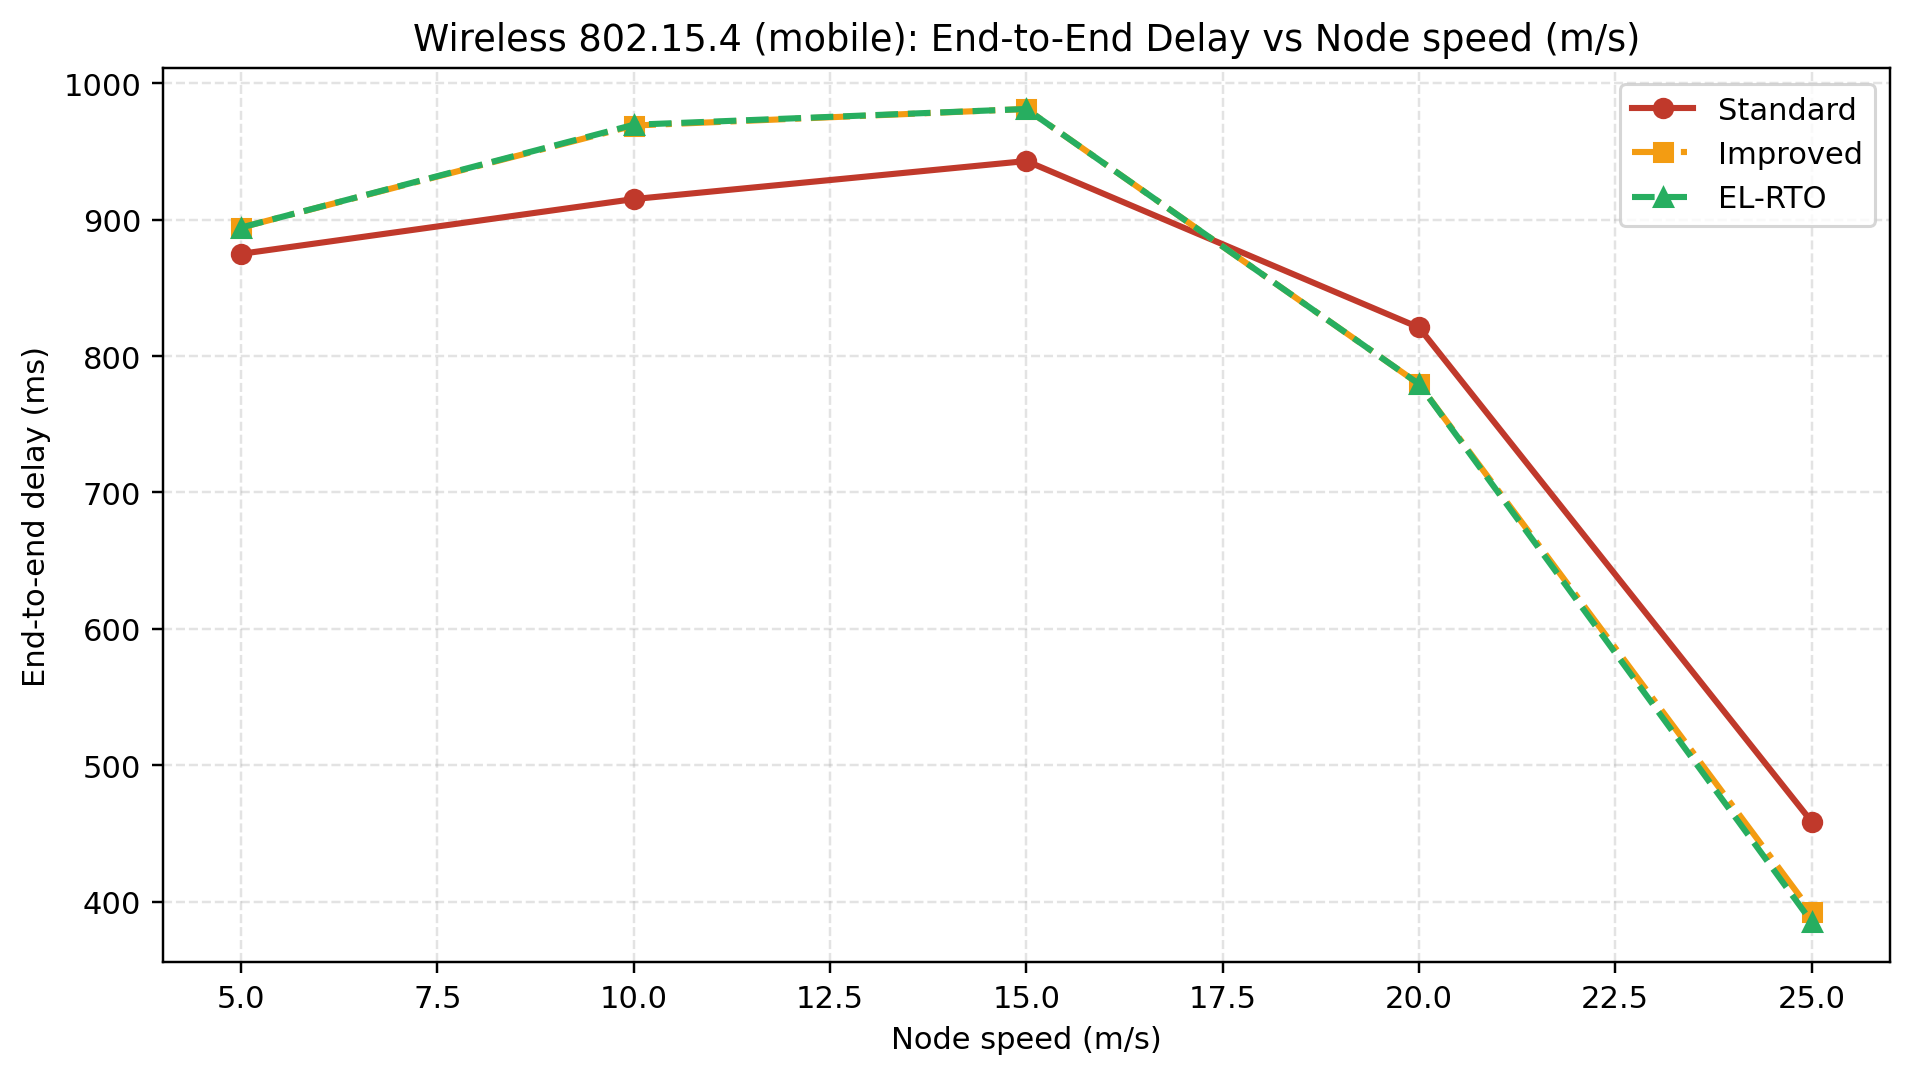
\includegraphics[width=\linewidth]{2105114_final_submission/lrwpan_mobile/student2105114_lrwpan_mobile_10s_plots/lrwpan-mobile_speed_averageDelayMs.png}
  \end{columns}

  \vspace{0.2cm}
  \footnotesize
  \begin{tabular}{lccc}
    \toprule
    Sweep & Mode & Avg Throughput & Avg Delay \\
    \midrule
    Nodes & Standard & 0.0614 & 761.298 \\
    Nodes & EL-RTO & 0.0642 & 630.646 \\
    Speed & Standard & 0.0593 & 802.523 \\
    Speed & EL-RTO & 0.0567 & 801.938 \\
    \bottomrule
  \end{tabular}

  \vspace{0.2cm}
  \begin{itemize}
    \item LR-WPAN throughput is much lower than Wi-Fi, as expected from the lower-capacity link layer.
    \item Under node variation, EL-RTO gave the best average delay and throughput among the three modes.
  \end{itemize}
\end{frame}

\begin{frame}{LR-WPAN Mobile: Reliability and Energy}
  \begin{columns}[T]
    \column{0.5\textwidth}
    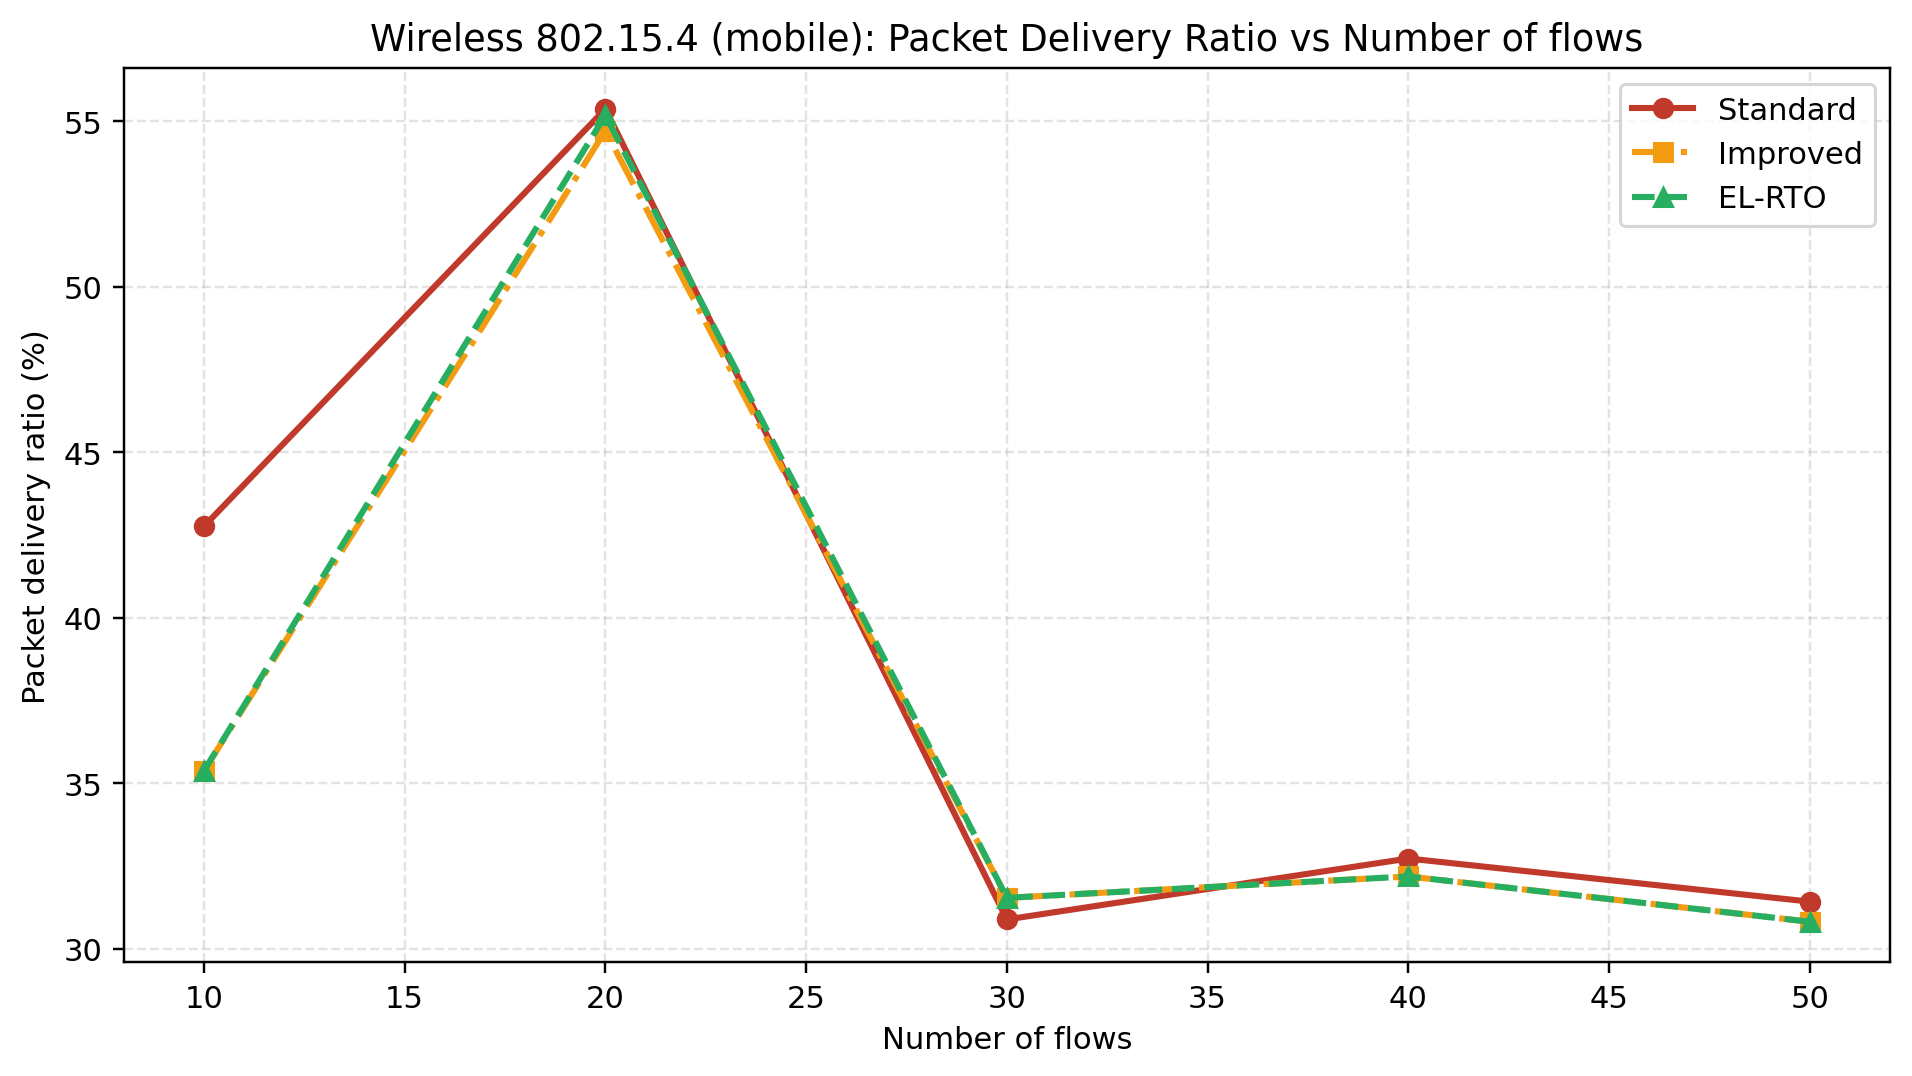
\includegraphics[width=\linewidth]{2105114_final_submission/lrwpan_mobile/student2105114_lrwpan_mobile_10s_plots/lrwpan-mobile_flows_pdrPct.png}

    \column{0.5\textwidth}
    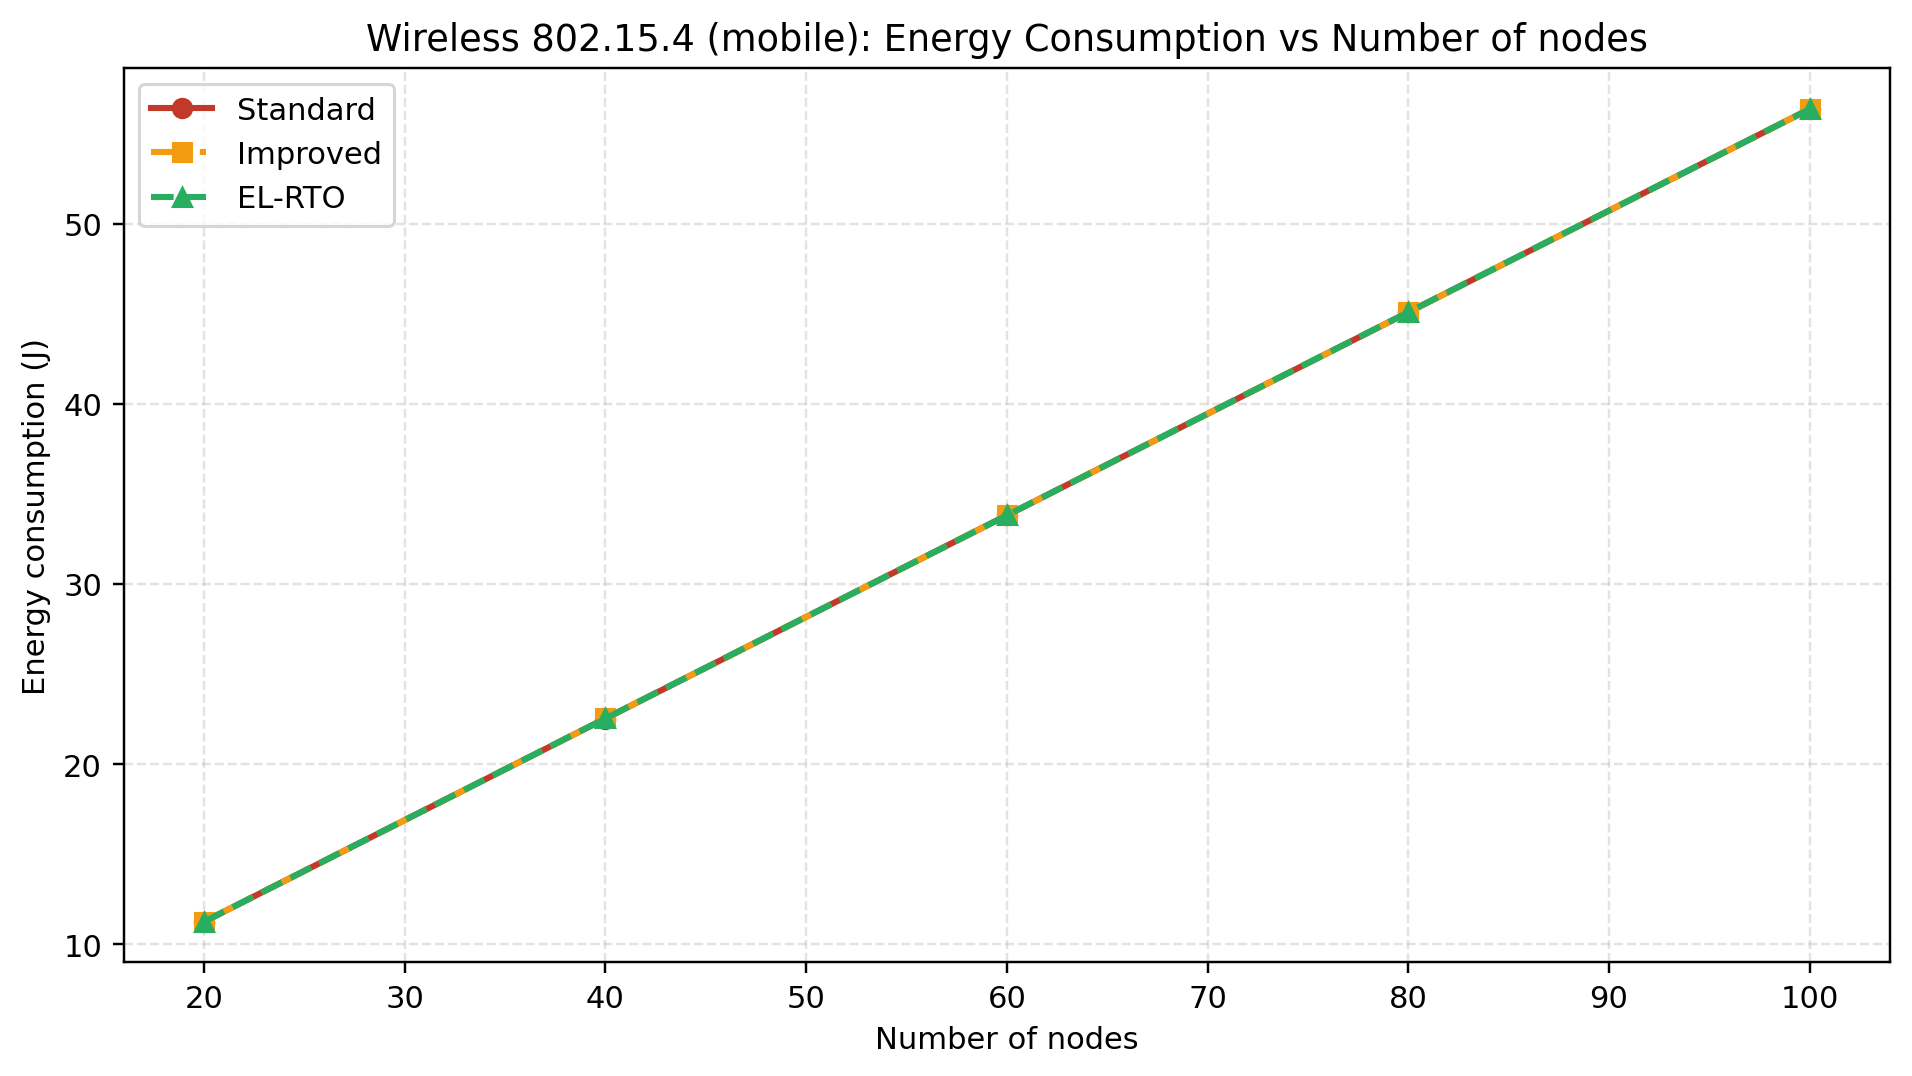
\includegraphics[width=\linewidth]{2105114_final_submission/lrwpan_mobile/student2105114_lrwpan_mobile_10s_plots/lrwpan-mobile_nodes_energyJ.png}
  \end{columns}

  \vspace{0.2cm}
  \footnotesize
  \begin{tabular}{lccc}
    \toprule
    Sweep & Mode & Avg PDR (\%) & Avg Energy (J) \\
    \midrule
    Nodes & Standard & 46.996 & 33.806 \\
    Nodes & EL-RTO & 48.772 & 33.807 \\
    Flows & Standard & 38.636 & 56.364 \\
    Flows & EL-RTO & 37.022 & 56.363 \\
    \bottomrule
  \end{tabular}
\end{frame}

\begin{frame}{Cross-Network Result Summary}
  \small
  \begin{tabular}{lcccc}
    \toprule
    Network & Condition & Best Mode & Key Gain & Observation \\
    \midrule
    Wi-Fi & Node sweep & Improved/EL-RTO & lower delay & very high PDR \\
    Wi-Fi & Flow sweep & Improved/EL-RTO & lower delay & curves overlap \\
    LR-WPAN & Node sweep & EL-RTO & higher throughput & lower delay \\
    LR-WPAN & Flow sweep & Standard/EL-RTO mixed & similar energy & loss remains high \\
    Spike test & induced spike & Improved/EL-RTO & lower peak RTO & tighter timer \\
    \bottomrule
  \end{tabular}

  \vspace{0.35cm}
  \begin{itemize}
    \item Wi-Fi benefits mostly in delay stability rather than dramatic throughput change.
    \item LR-WPAN is much more constrained, so timer improvements appear in finer-grained behavior.
    \item EL-RTO is most convincing in the explicit spike experiment.
  \end{itemize}
\end{frame}

\begin{frame}{Discussion and Reflection}
  \begin{itemize}
    \item The \textbf{base-paper reproduction} confirmed the main timer-tracking idea: the improved estimator reduces the average RTO-RTT deviation during RTT increase, which means the estimator follows changing path conditions more closely.
    \item The \textbf{spike experiment} showed the clearest motivation for EL-RTO. When a short burst created temporary congestion, the standard estimator inflated RTO more than the improved and EL-RTO variants.
    \item In the \textbf{Wi-Fi mobile checklist runs}, the link layer was strong enough that all modes kept very high delivery ratios. As a result, timer changes affected delay behavior more than raw throughput.
    \item In the \textbf{LR-WPAN mobile checklist runs}, the network was much more resource-constrained. Here the transport timer still mattered, but overall performance was dominated by lower bandwidth, mobility, and contention.
    \item A practical observation from the results is that \textbf{transport-layer timer improvements do not always produce dramatic throughput gains}. Their benefit is often seen in tighter RTO control, lower overshoot, and sometimes lower delay.
    \item Another important reflection is that \textbf{algorithmic improvement and wireless realism must be balanced}. The final Wi-Fi setup had to be simplified to a stable infrastructure topology so the checklist experiment would produce meaningful data instead of repeated zero-throughput failures.
    \item From a systems perspective, the project shows that \textbf{RTO design matters most when RTT changes are abrupt or noisy}. In stable conditions, the difference between improved and EL-RTO can become very small, which is why several checklist curves overlap.
  \end{itemize}
\end{frame}

\begin{frame}{Interpretation for Supervisor Discussion}
  \begin{itemize}
    \item \textbf{What worked best:}
    \begin{itemize}
      \item improved and EL-RTO reduced timer inflation in controlled scenarios
      \item EL-RTO was most justified in explicit spike conditions
      \item the checklist automation made large experiment sweeps repeatable
    \end{itemize}
    \item \textbf{What limited the gains:}
    \begin{itemize}
      \item wireless contention and link capacity often dominated performance
      \item mobile wireless behavior introduced noise beyond just RTT-estimation effects
      \item laptop resource constraints required reducing checklist simulation time to 10 seconds
    \end{itemize}
    \item \textbf{Main takeaway:}
    \begin{itemize}
      \item the project successfully demonstrates the timer-level advantage of the improved and EL-RTO methods
      \item end-to-end network gains depend strongly on the surrounding wireless environment
    \end{itemize}
  \end{itemize}
\end{frame}

\appendix
\section{Appendix: All Checklist Plots}

\begin{frame}{Wi-Fi Mobile: Node Sweep}
  \centering
  \begin{tabular}{cc}
    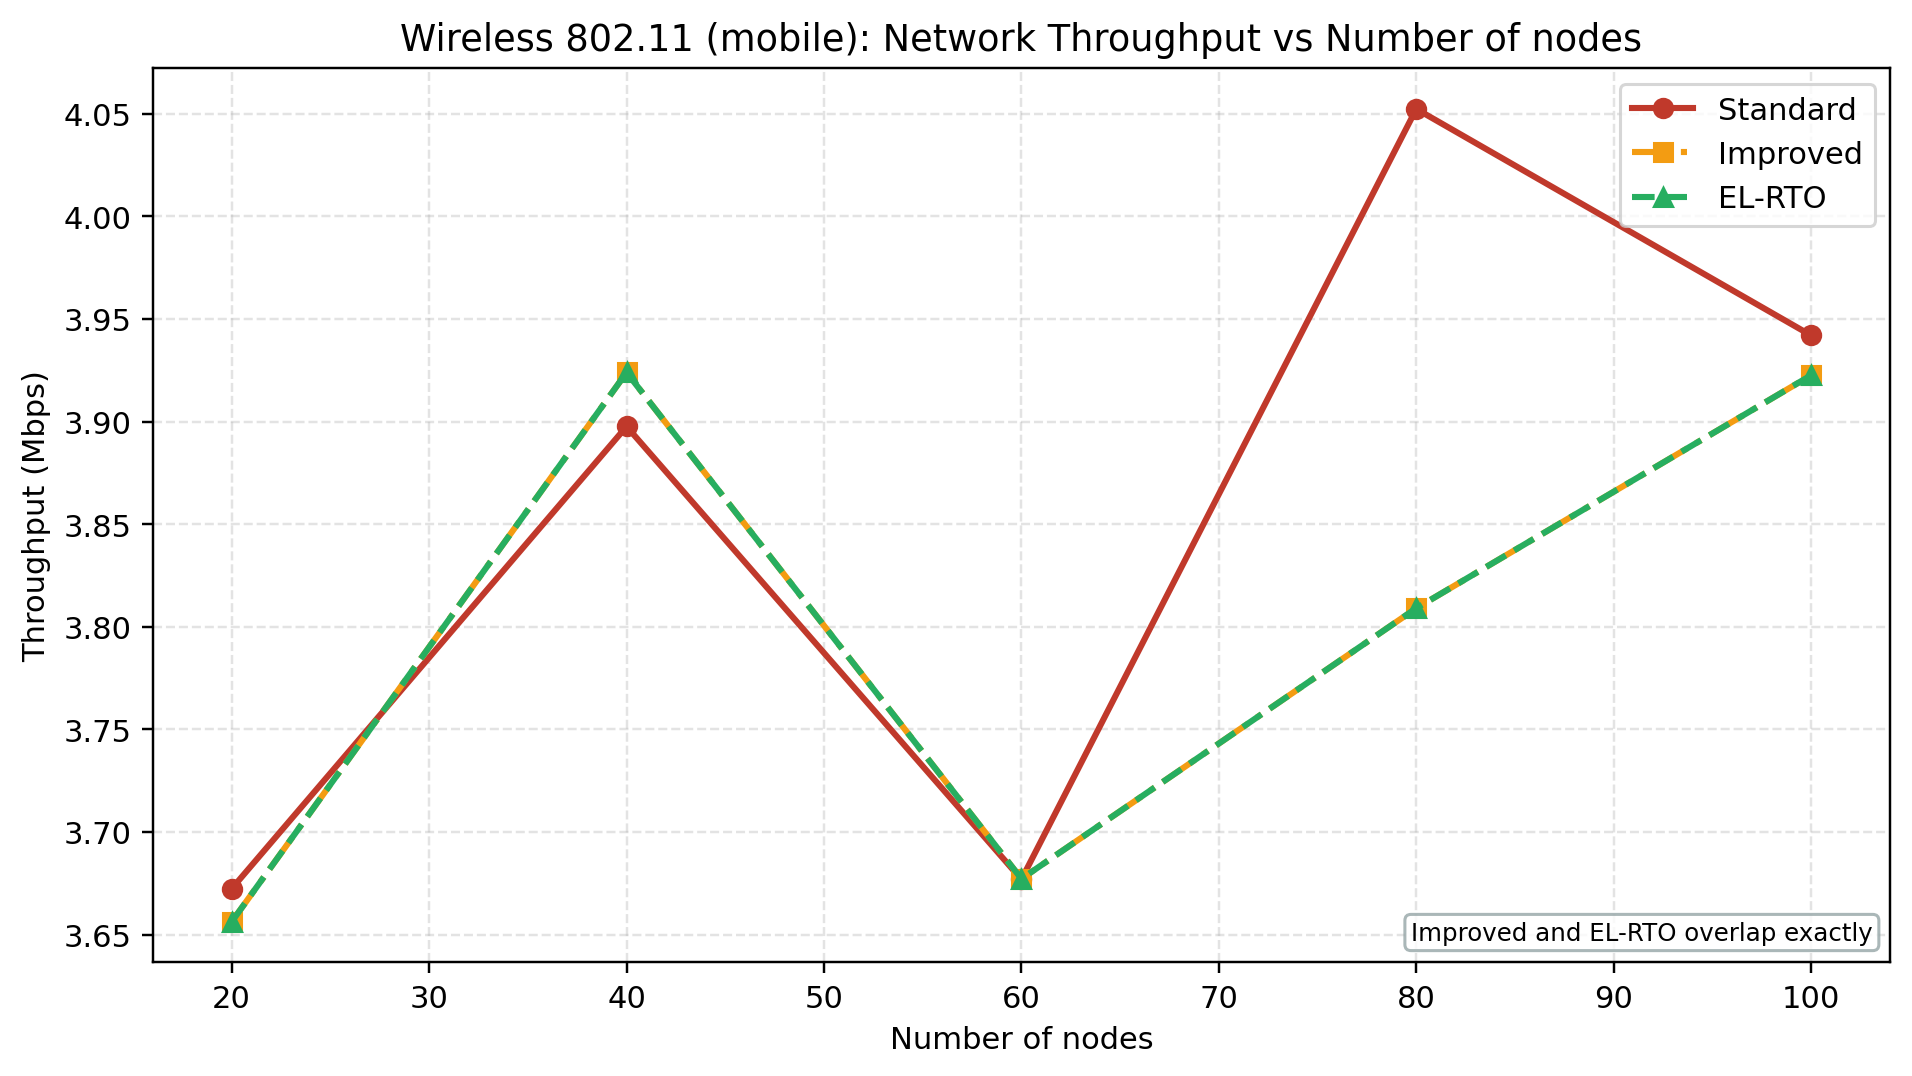
\includegraphics[width=0.47\linewidth]{2105114_final_submission/wifi_mobile/student2105114_wifi_mobile_10s_plots/wifi-mobile_nodes_throughputMbps.png} &
    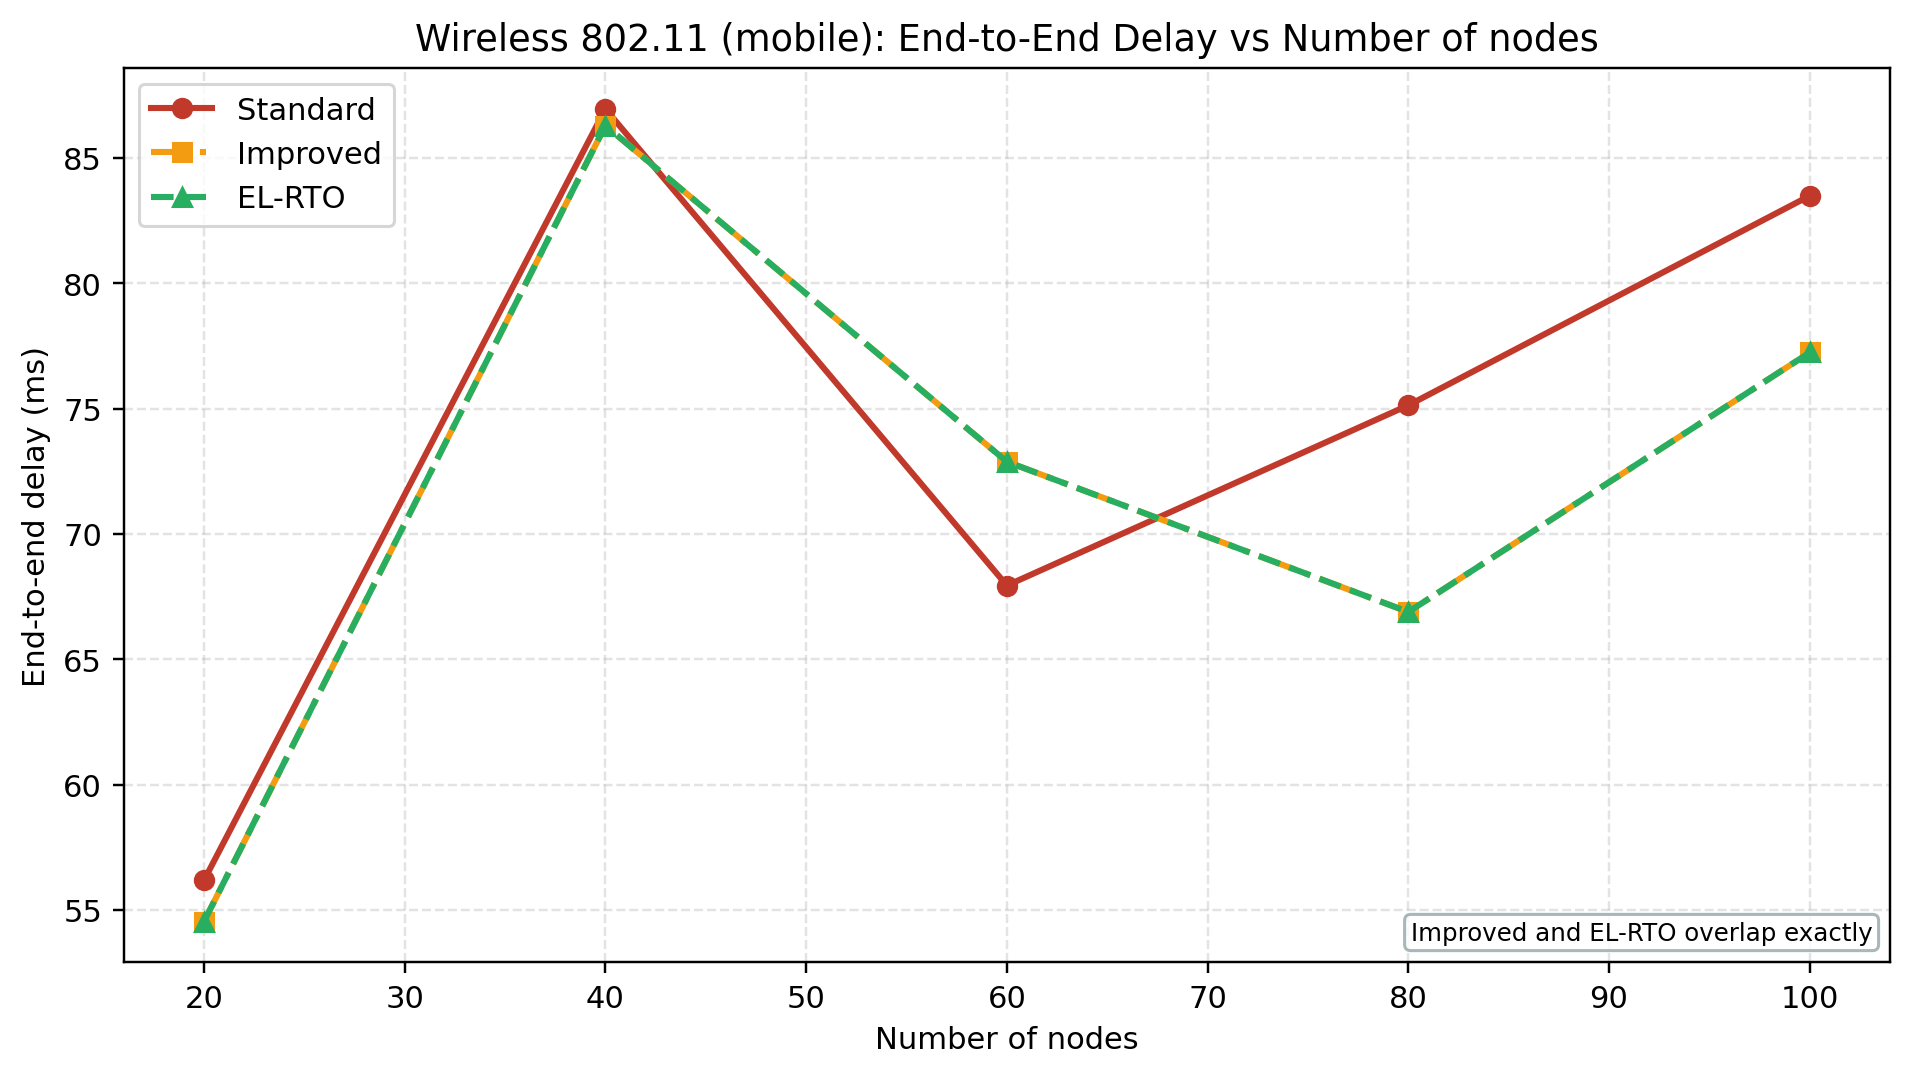
\includegraphics[width=0.47\linewidth]{2105114_final_submission/wifi_mobile/student2105114_wifi_mobile_10s_plots/wifi-mobile_nodes_averageDelayMs.png} \\
    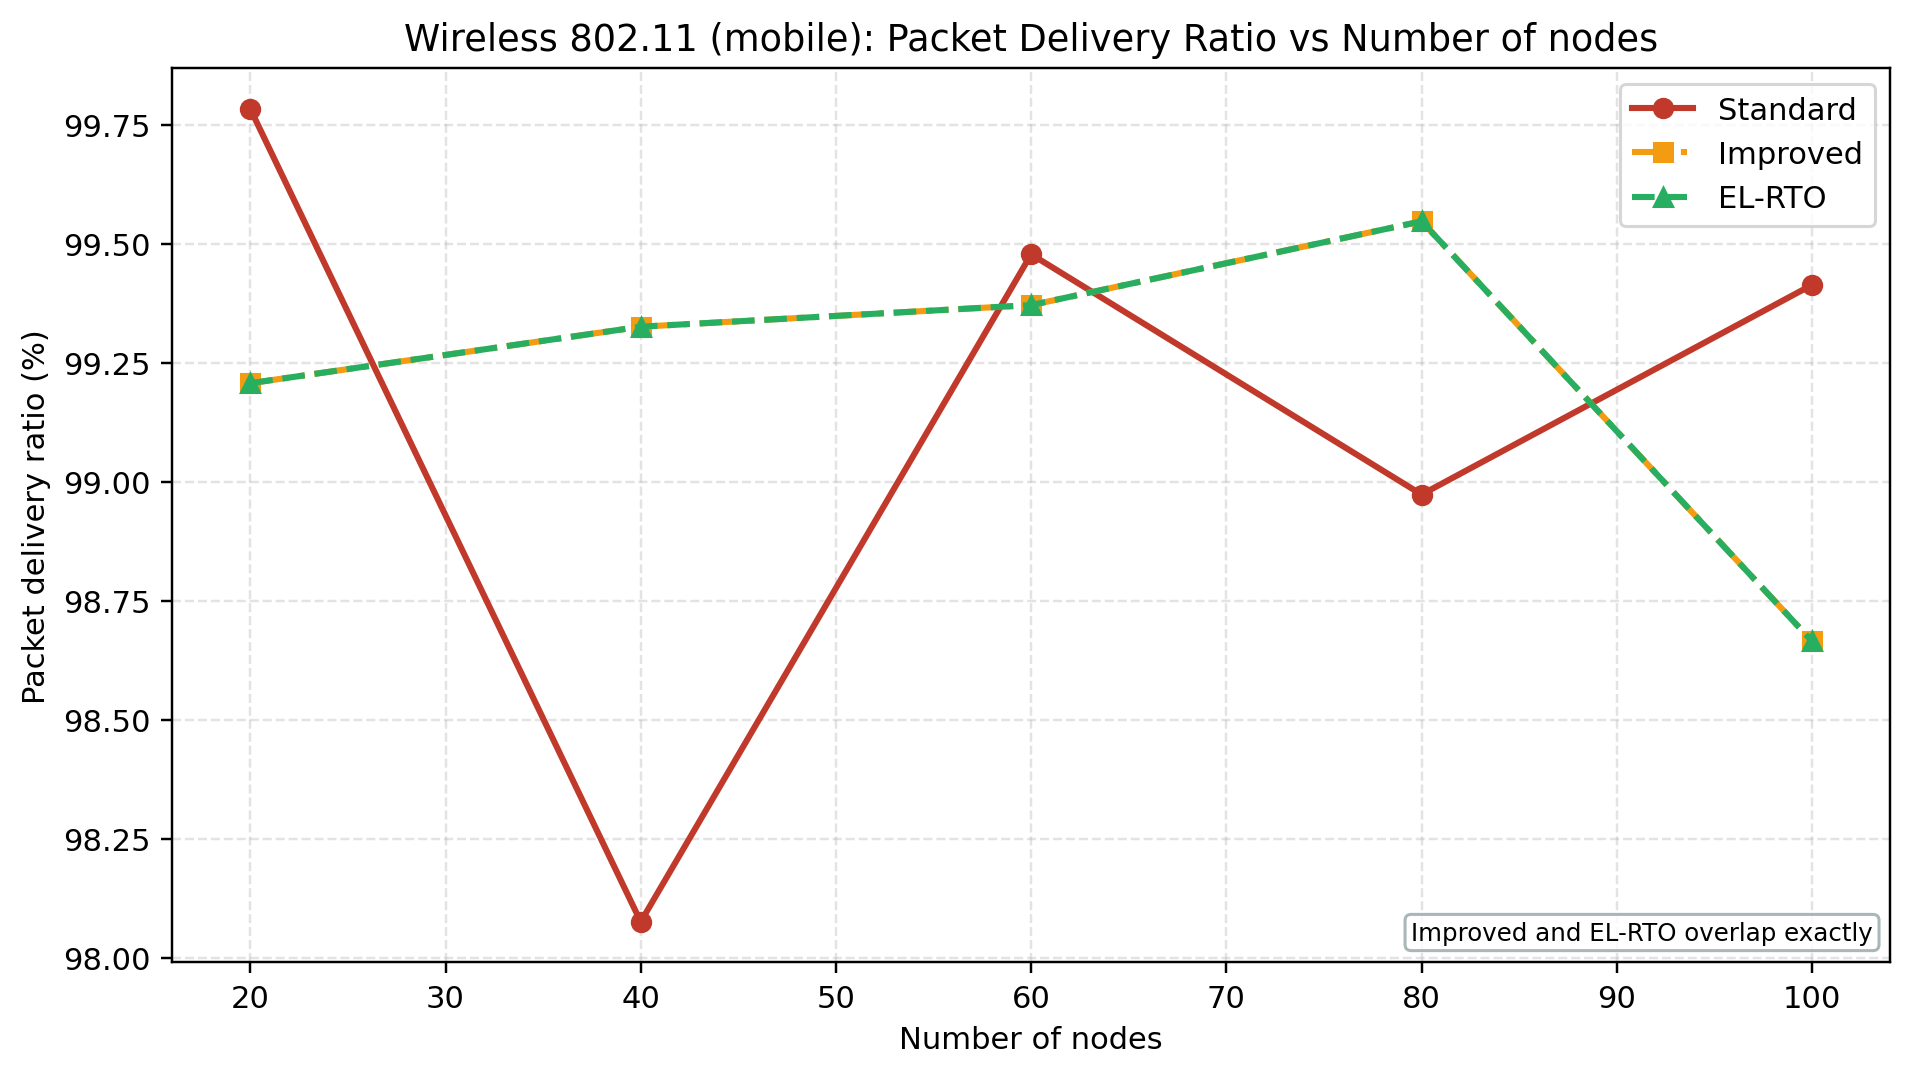
\includegraphics[width=0.47\linewidth]{2105114_final_submission/wifi_mobile/student2105114_wifi_mobile_10s_plots/wifi-mobile_nodes_pdrPct.png} &
    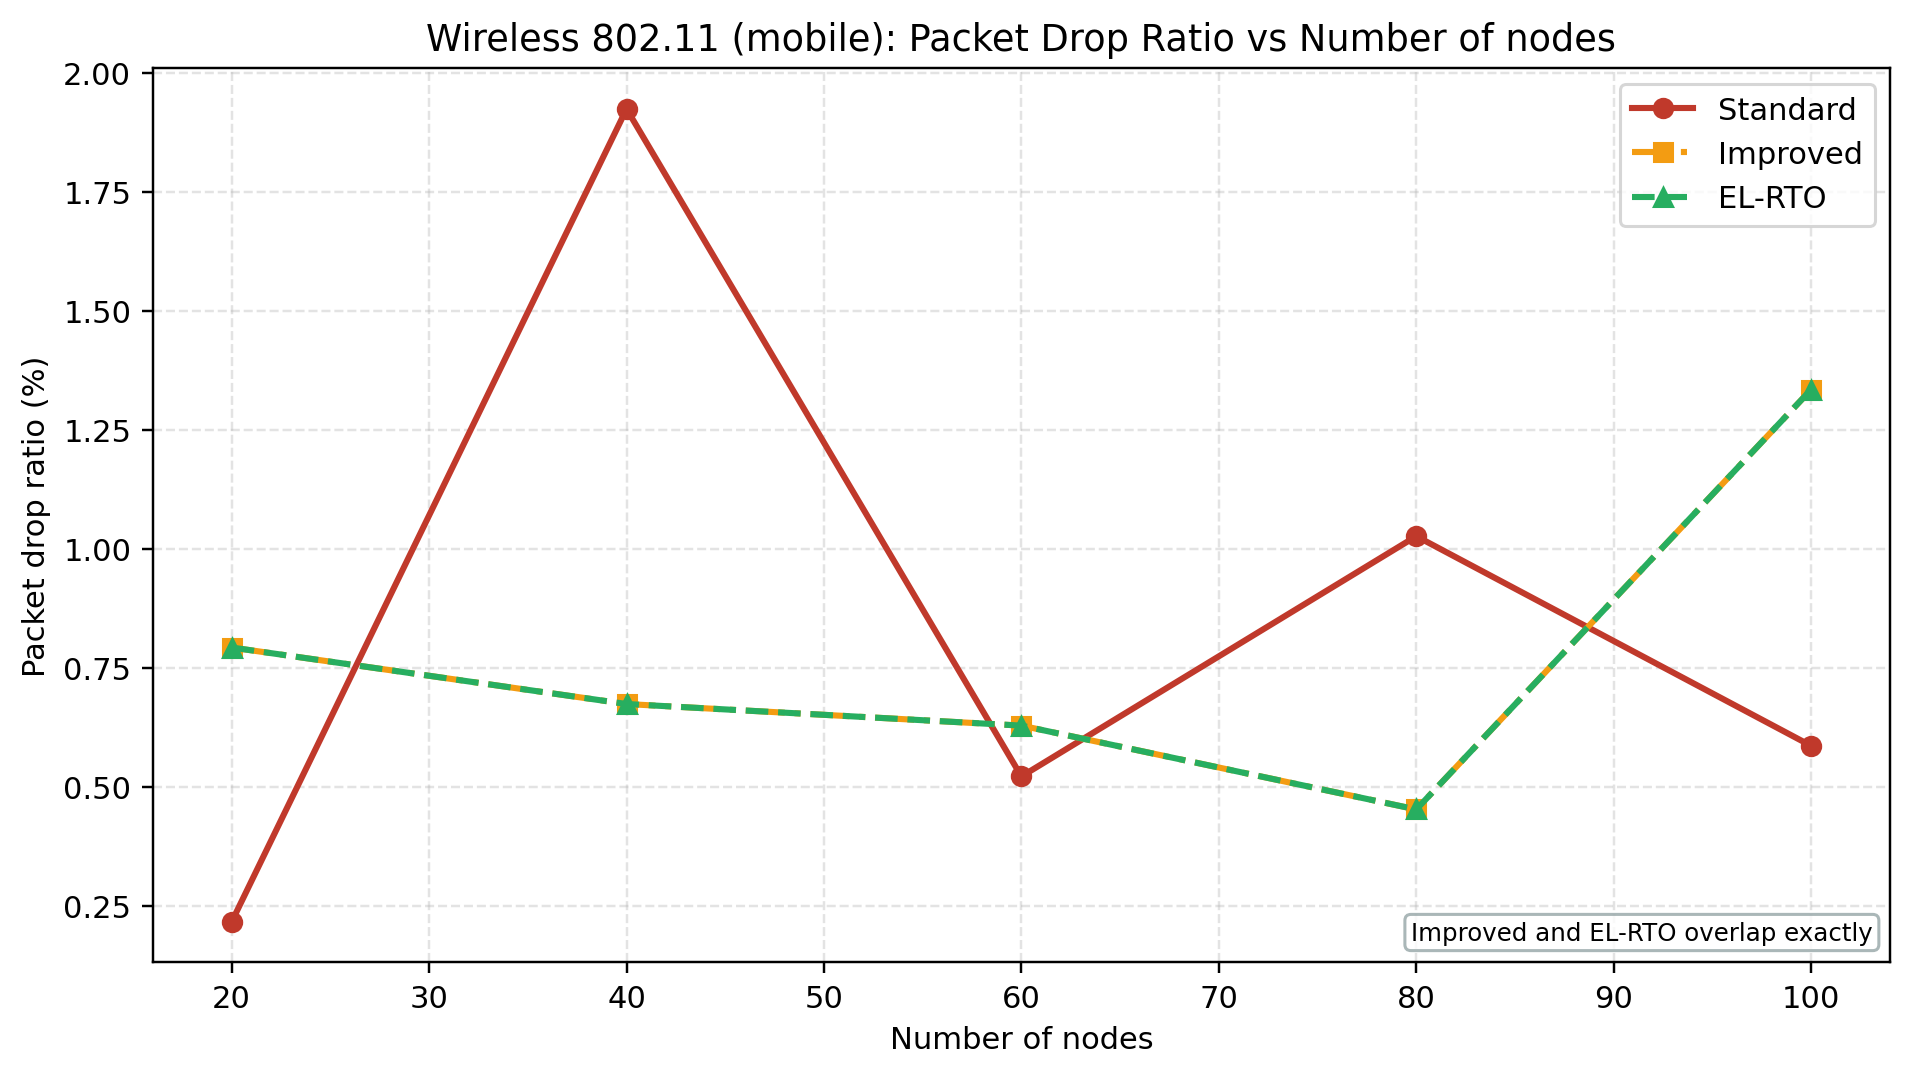
\includegraphics[width=0.47\linewidth]{2105114_final_submission/wifi_mobile/student2105114_wifi_mobile_10s_plots/wifi-mobile_nodes_dropRatioPct.png}
  \end{tabular}

  \vspace{0.15cm}
  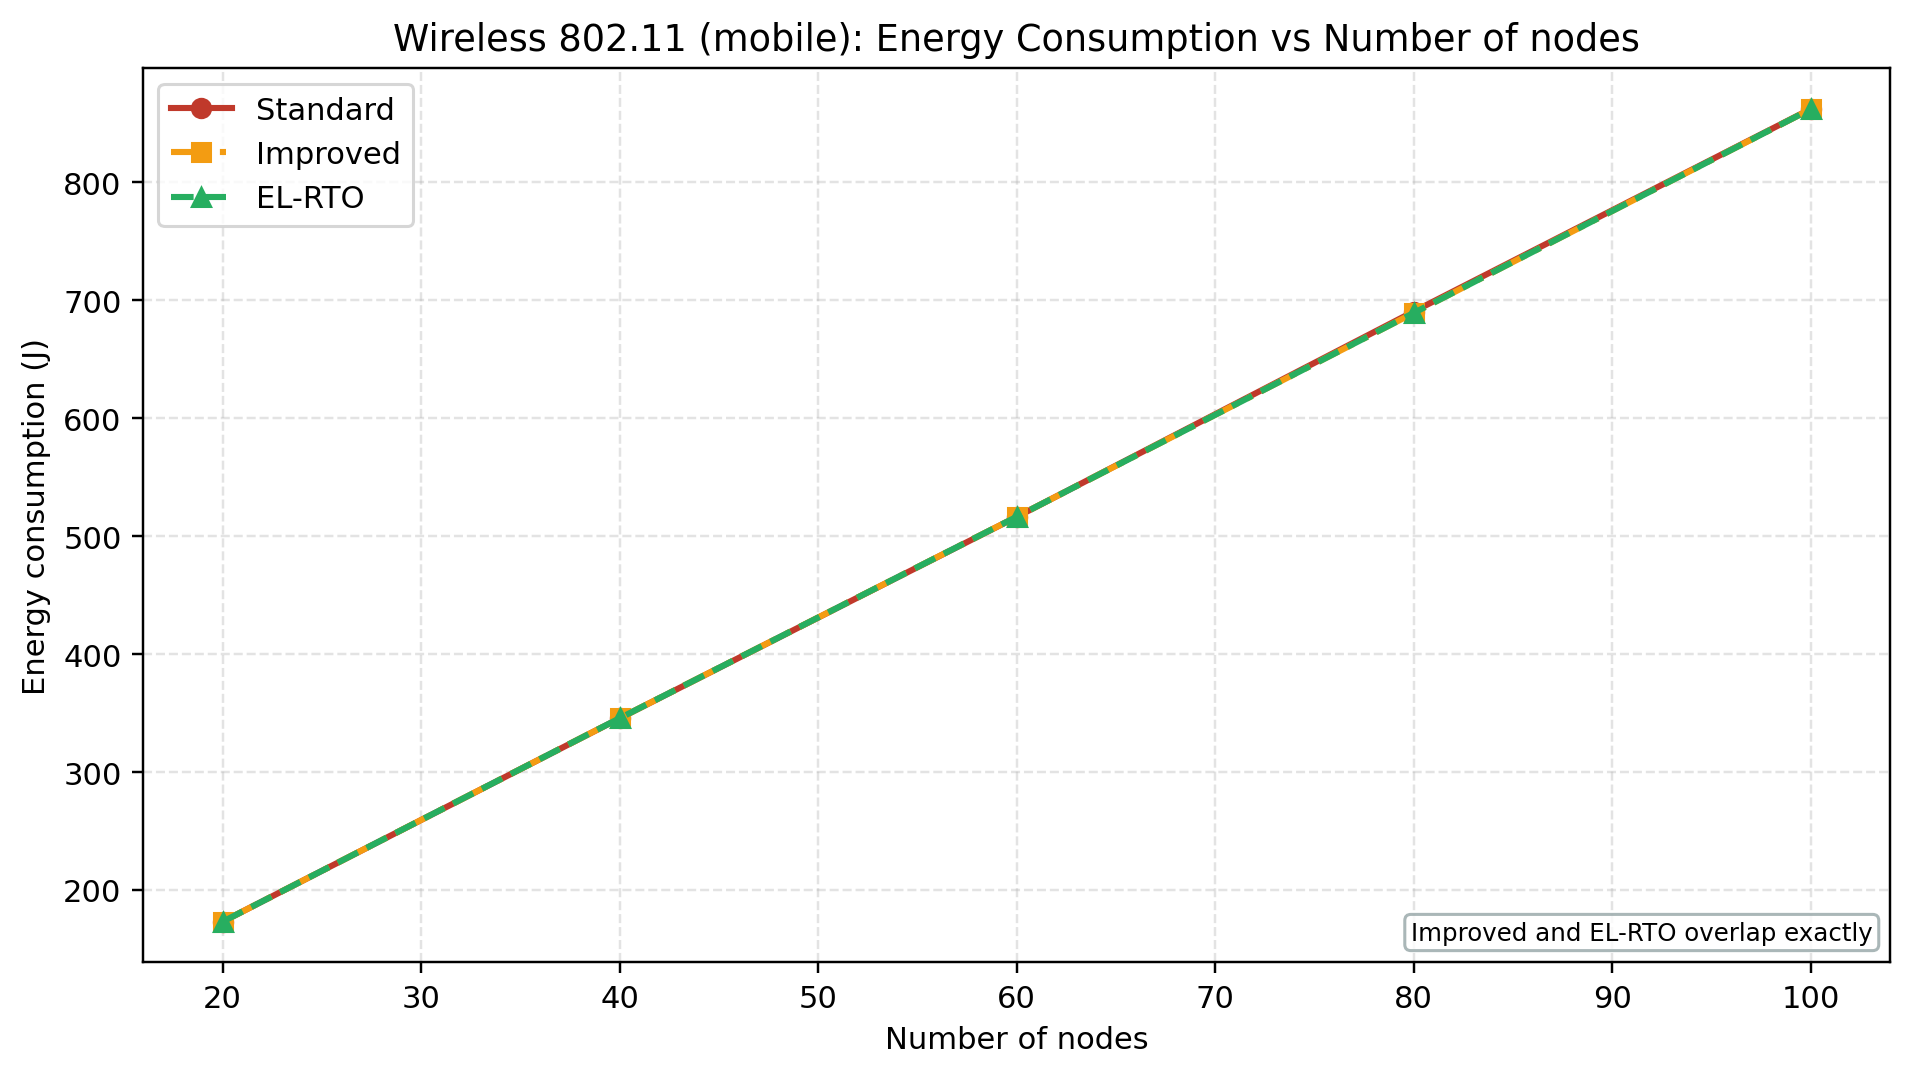
\includegraphics[width=0.47\linewidth]{2105114_final_submission/wifi_mobile/student2105114_wifi_mobile_10s_plots/wifi-mobile_nodes_energyJ.png}
\end{frame}

\begin{frame}{Wi-Fi Mobile: Flow Sweep}
  \centering
  \begin{tabular}{cc}
    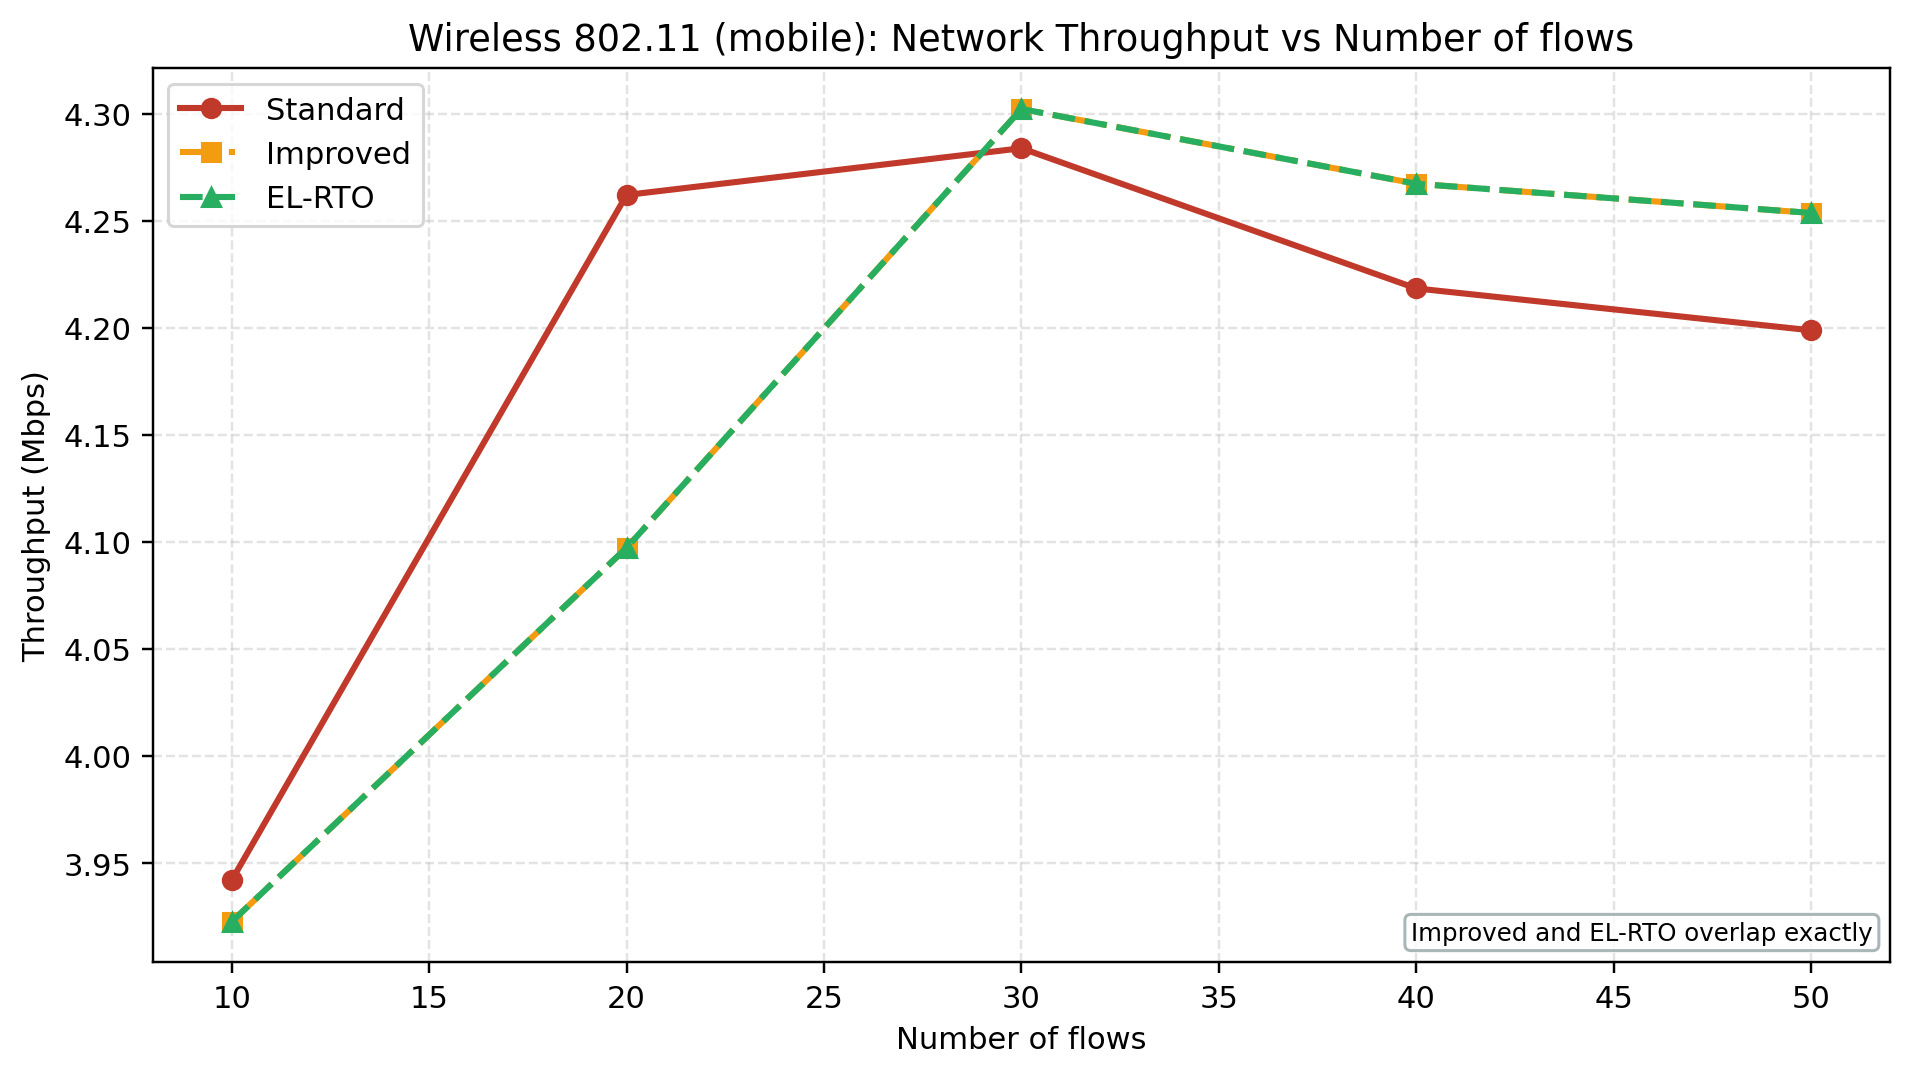
\includegraphics[width=0.47\linewidth]{2105114_final_submission/wifi_mobile/student2105114_wifi_mobile_10s_plots/wifi-mobile_flows_throughputMbps.png} &
    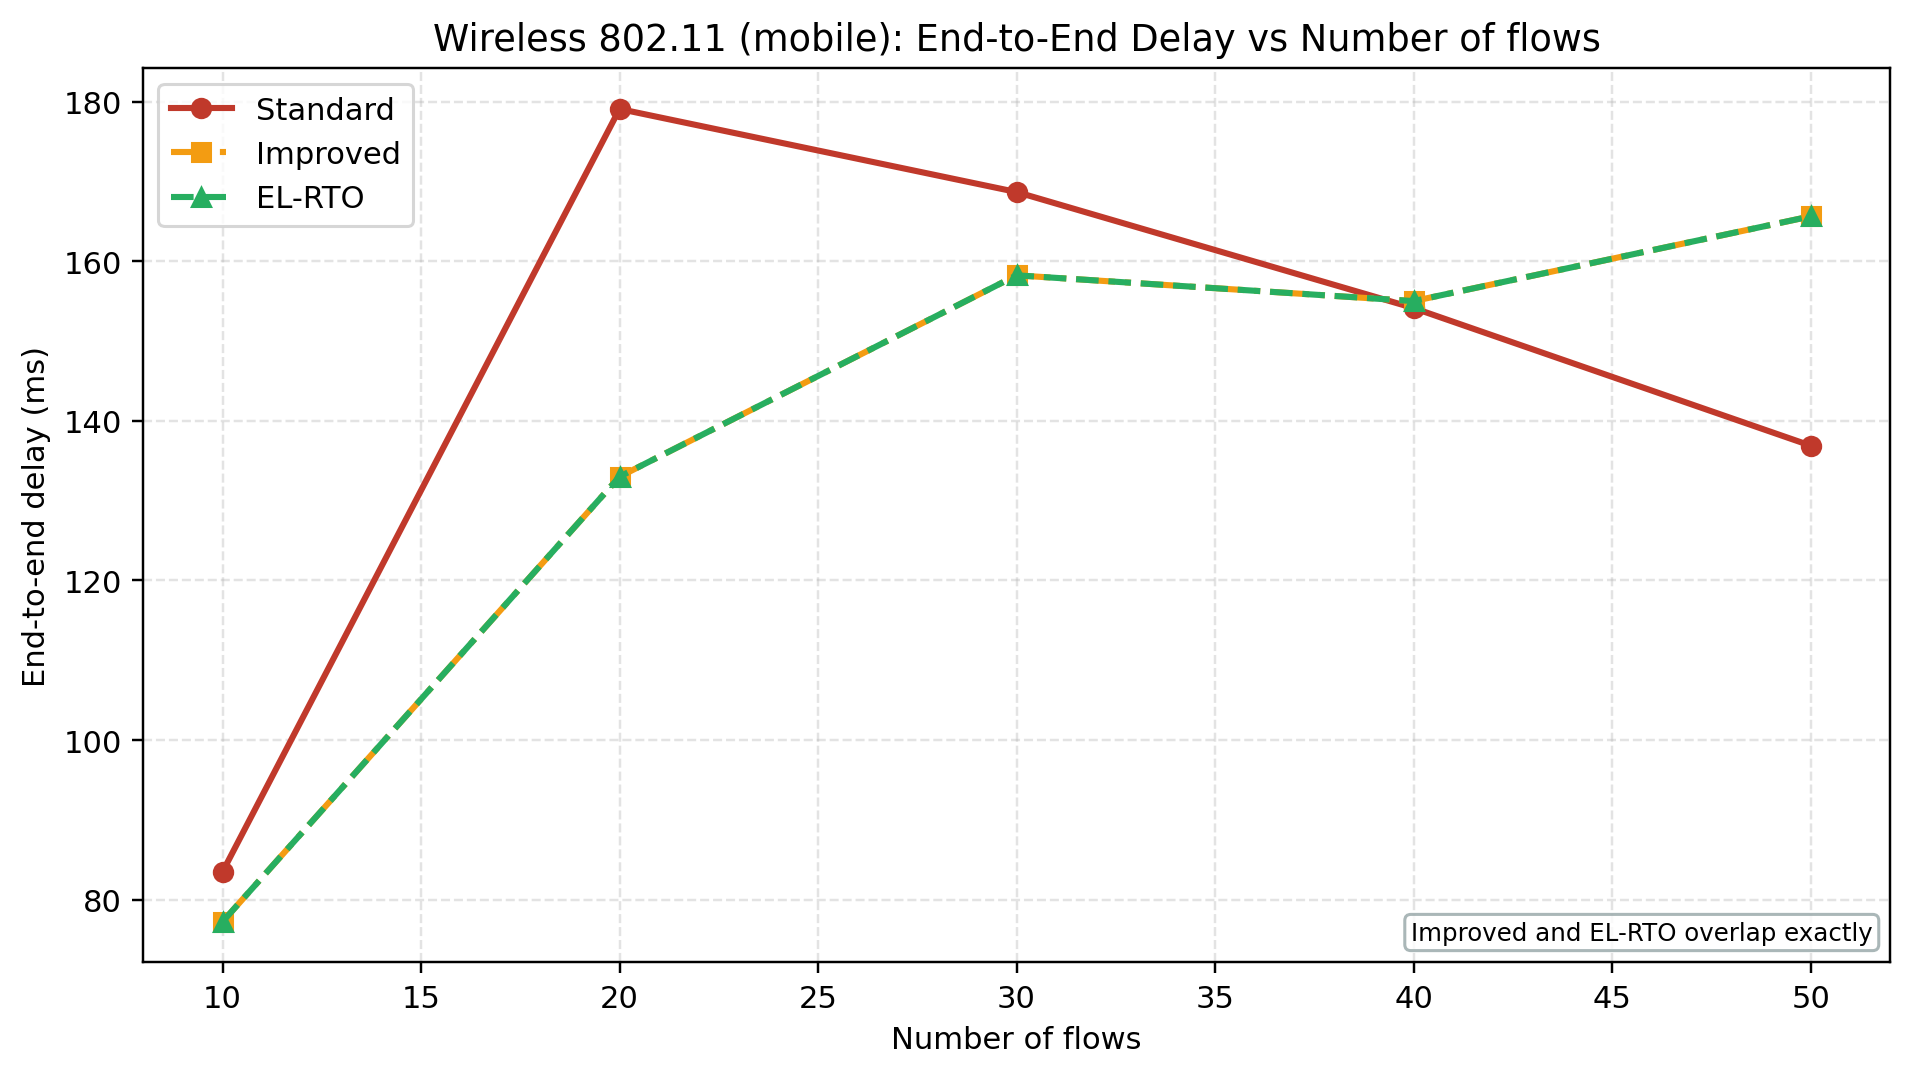
\includegraphics[width=0.47\linewidth]{2105114_final_submission/wifi_mobile/student2105114_wifi_mobile_10s_plots/wifi-mobile_flows_averageDelayMs.png} \\
    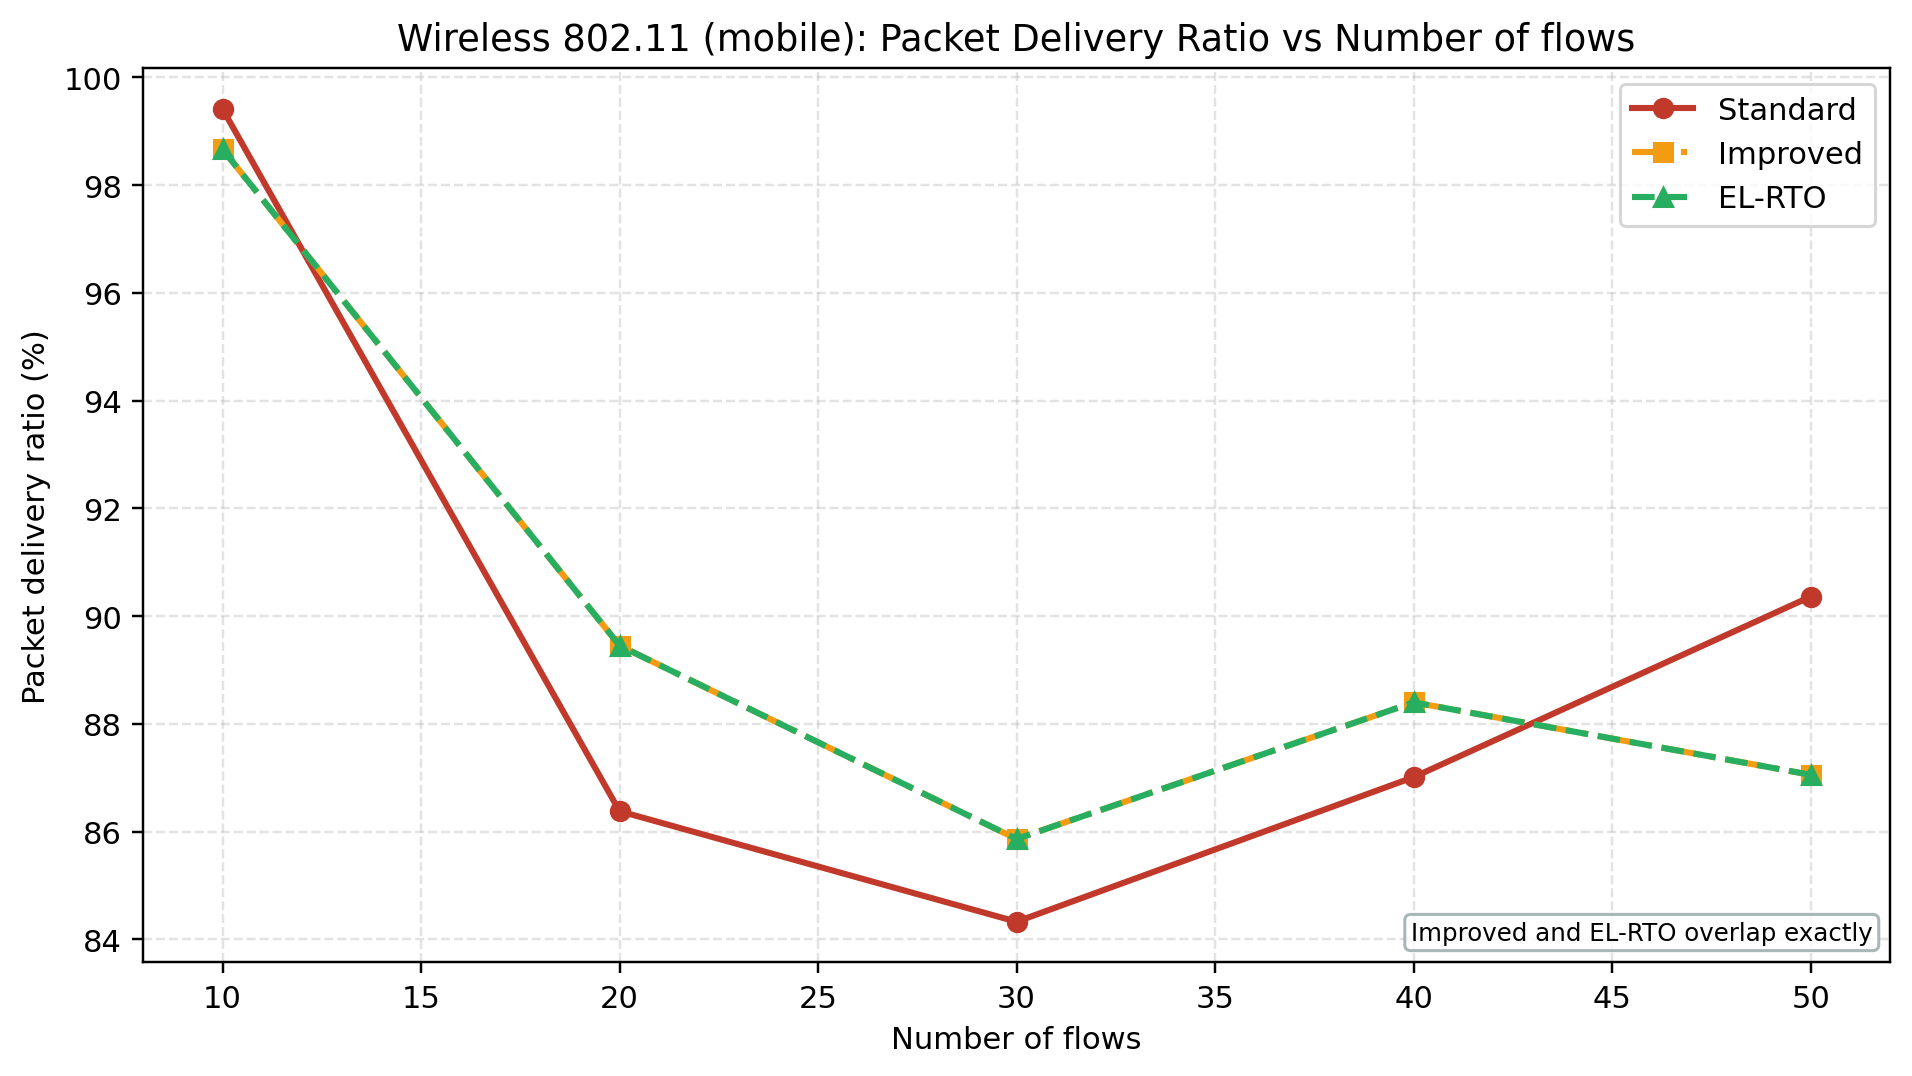
\includegraphics[width=0.47\linewidth]{2105114_final_submission/wifi_mobile/student2105114_wifi_mobile_10s_plots/wifi-mobile_flows_pdrPct.png} &
    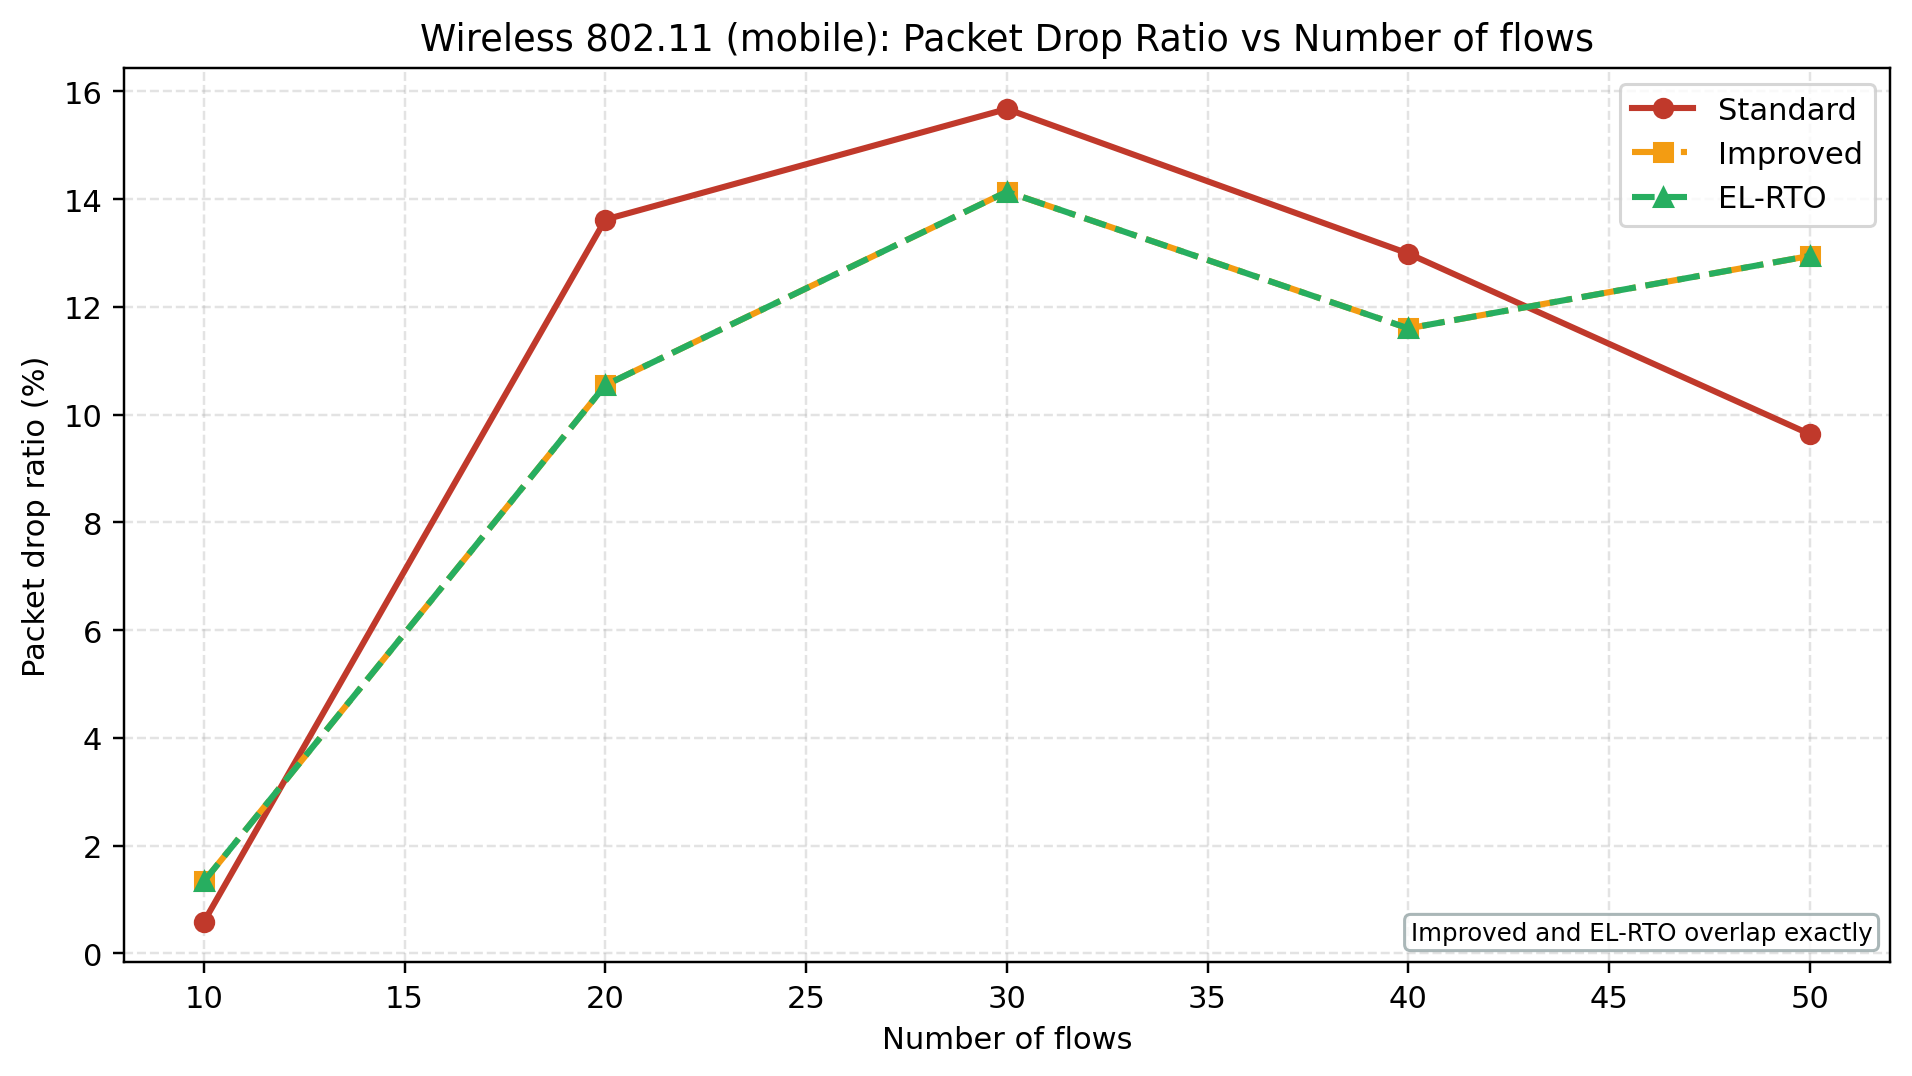
\includegraphics[width=0.47\linewidth]{2105114_final_submission/wifi_mobile/student2105114_wifi_mobile_10s_plots/wifi-mobile_flows_dropRatioPct.png}
  \end{tabular}

  \vspace{0.15cm}
  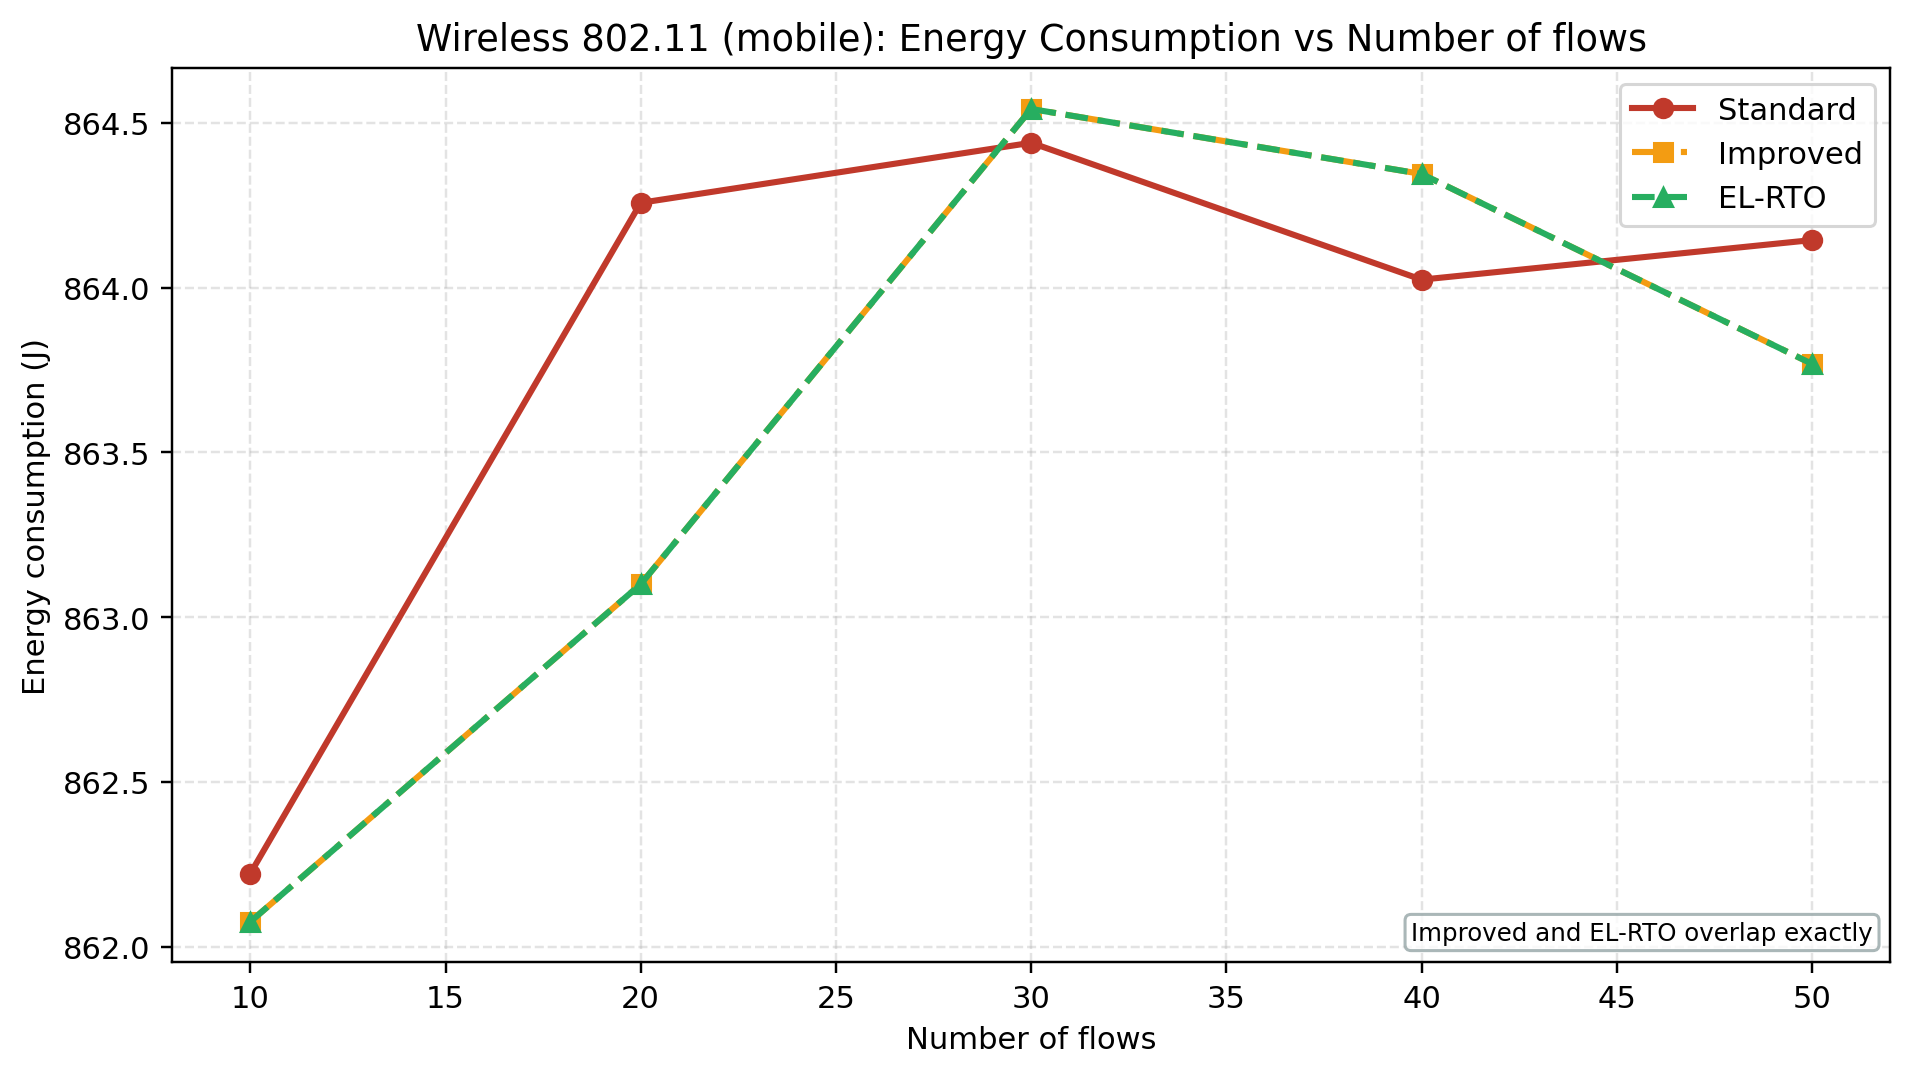
\includegraphics[width=0.47\linewidth]{2105114_final_submission/wifi_mobile/student2105114_wifi_mobile_10s_plots/wifi-mobile_flows_energyJ.png}
\end{frame}

\begin{frame}{Wi-Fi Mobile: Packet-Rate Sweep}
  \centering
  \begin{tabular}{cc}
    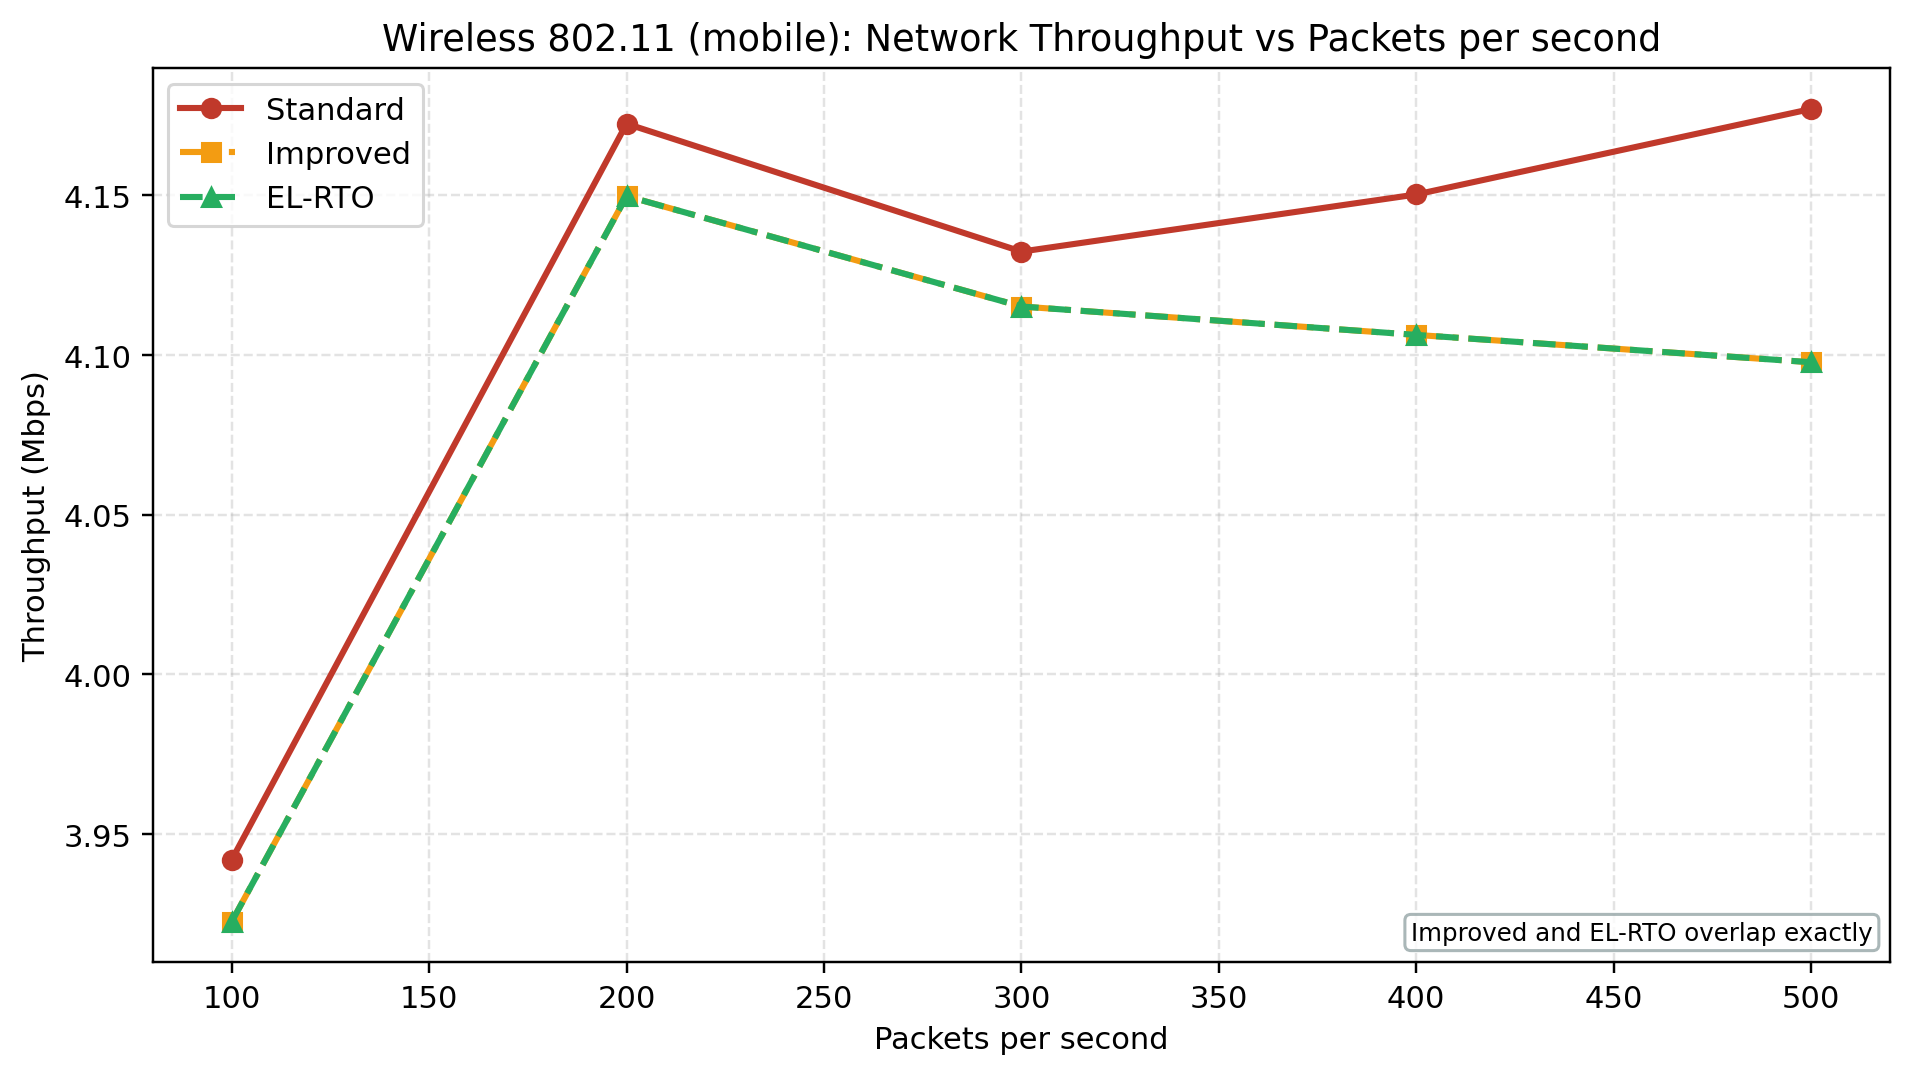
\includegraphics[width=0.47\linewidth]{2105114_final_submission/wifi_mobile/student2105114_wifi_mobile_10s_plots/wifi-mobile_pps_throughputMbps.png} &
    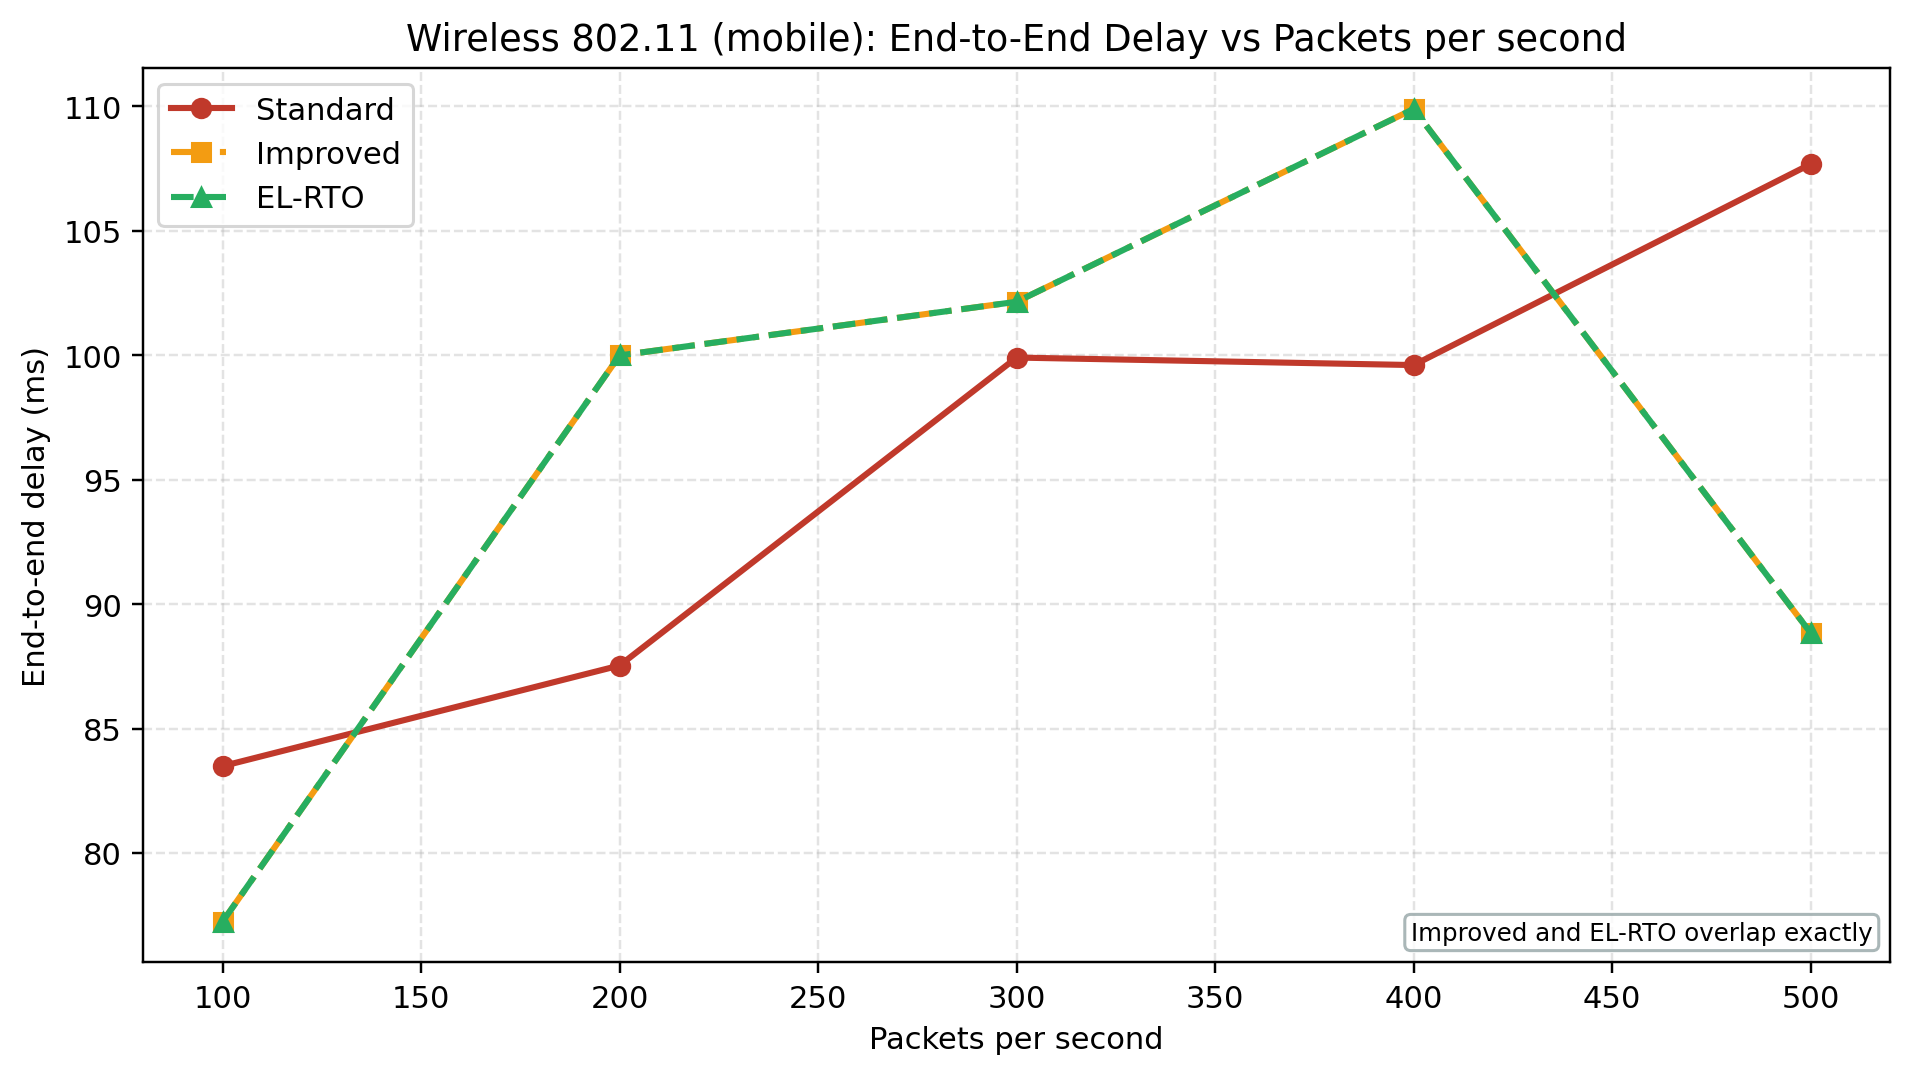
\includegraphics[width=0.47\linewidth]{2105114_final_submission/wifi_mobile/student2105114_wifi_mobile_10s_plots/wifi-mobile_pps_averageDelayMs.png} \\
    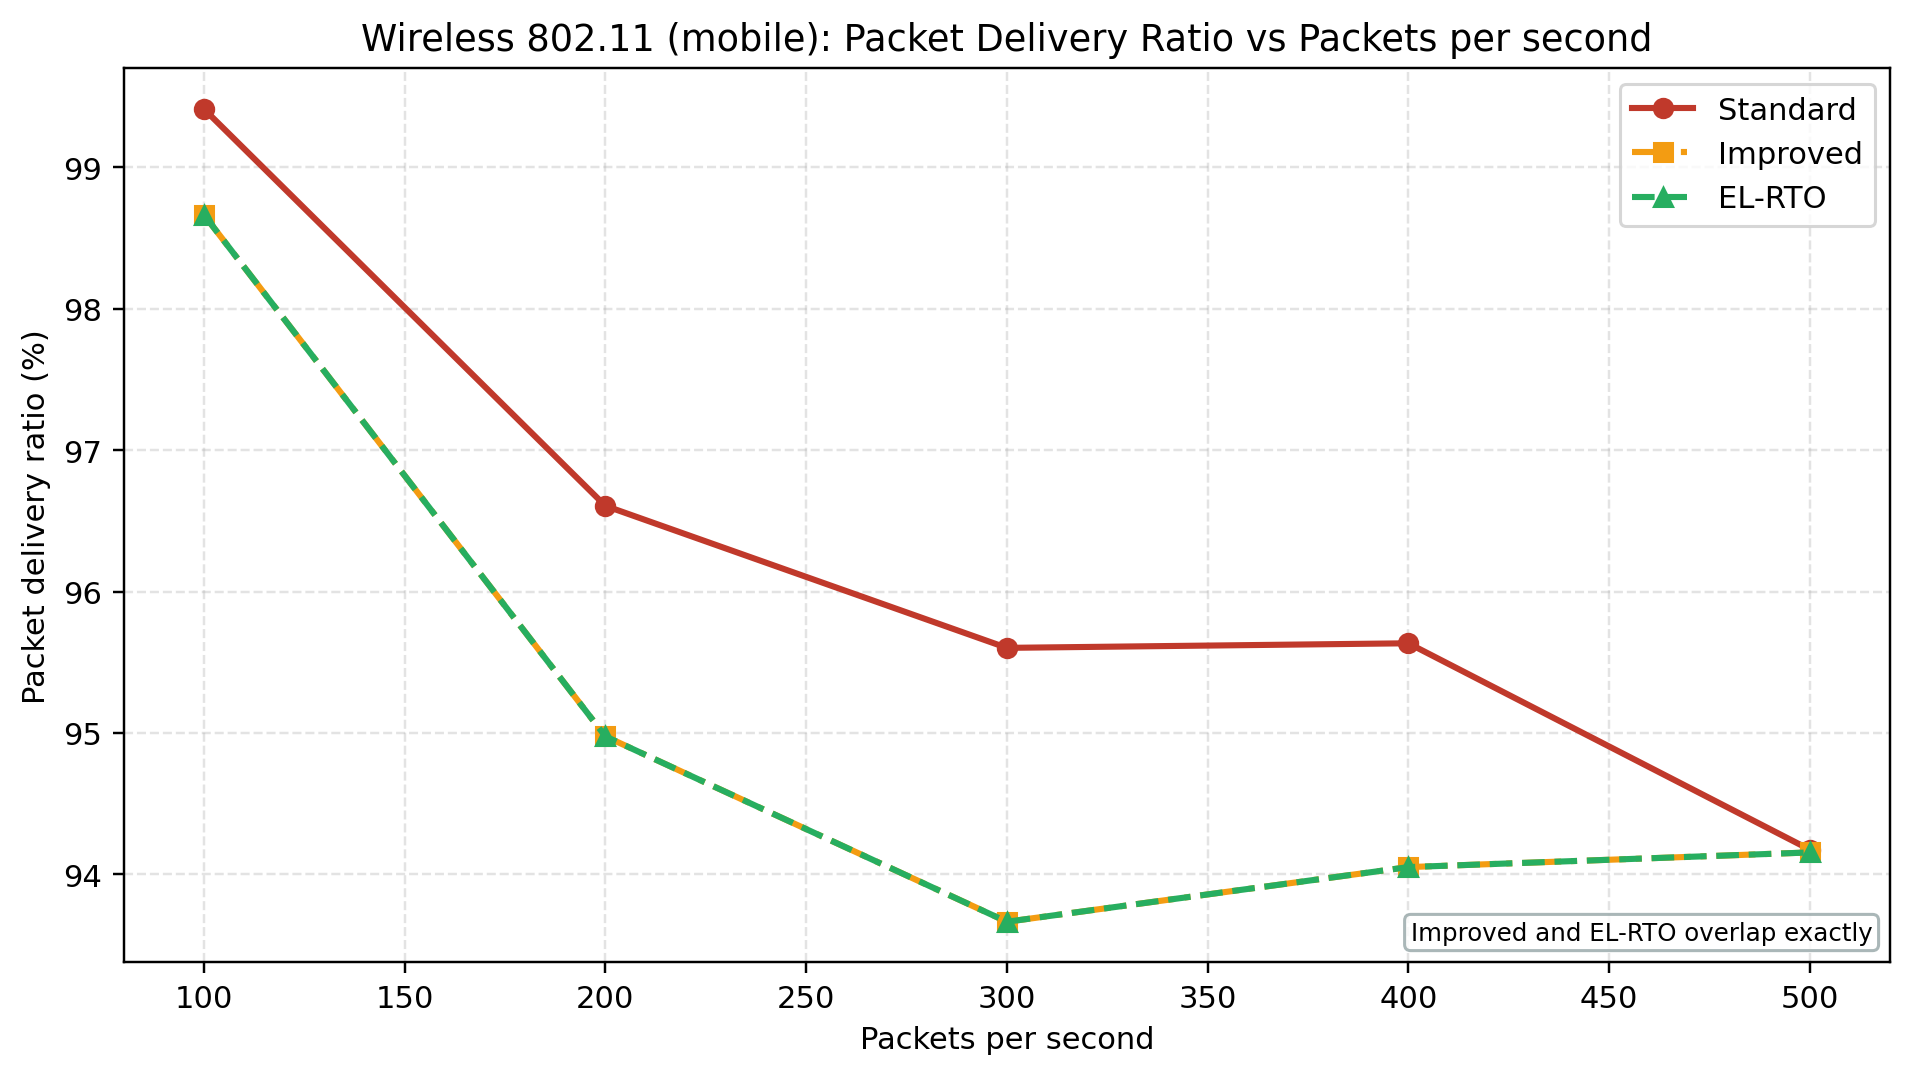
\includegraphics[width=0.47\linewidth]{2105114_final_submission/wifi_mobile/student2105114_wifi_mobile_10s_plots/wifi-mobile_pps_pdrPct.png} &
    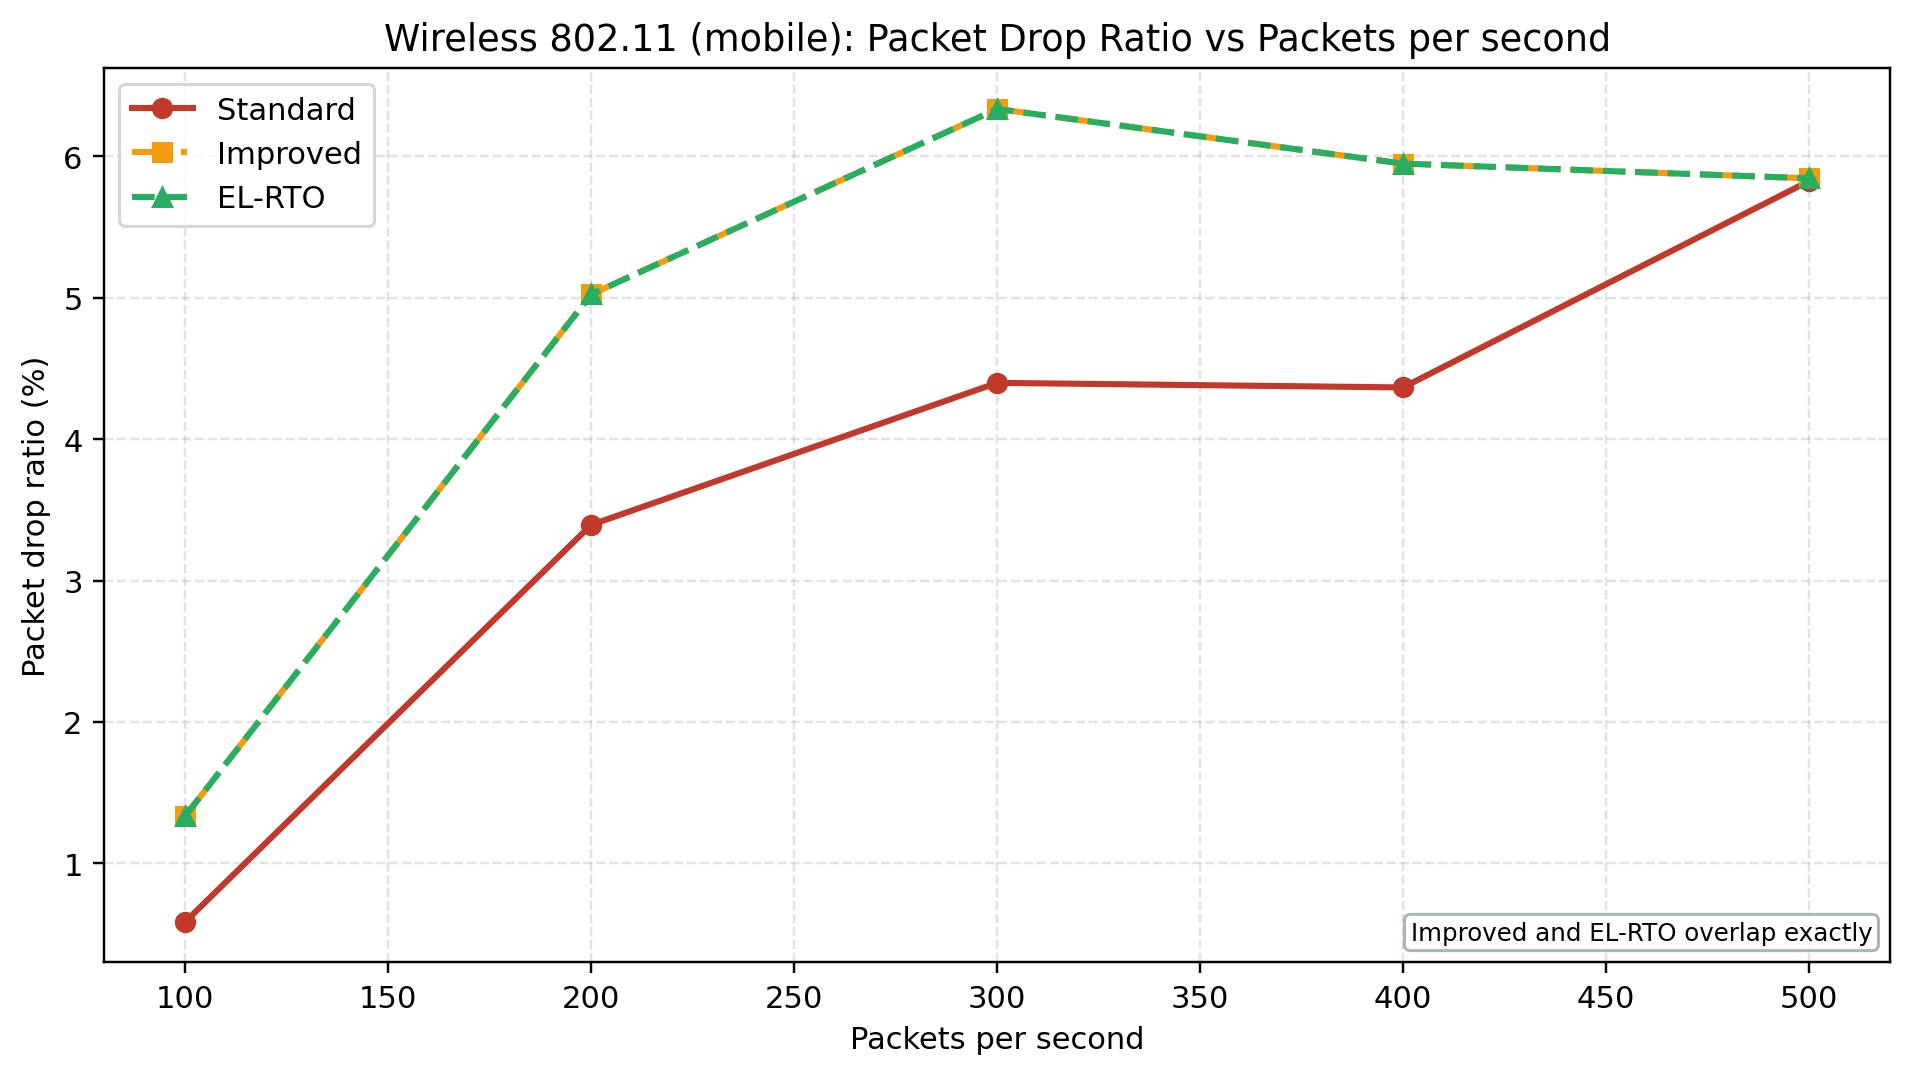
\includegraphics[width=0.47\linewidth]{2105114_final_submission/wifi_mobile/student2105114_wifi_mobile_10s_plots/wifi-mobile_pps_dropRatioPct.png}
  \end{tabular}

  \vspace{0.15cm}
  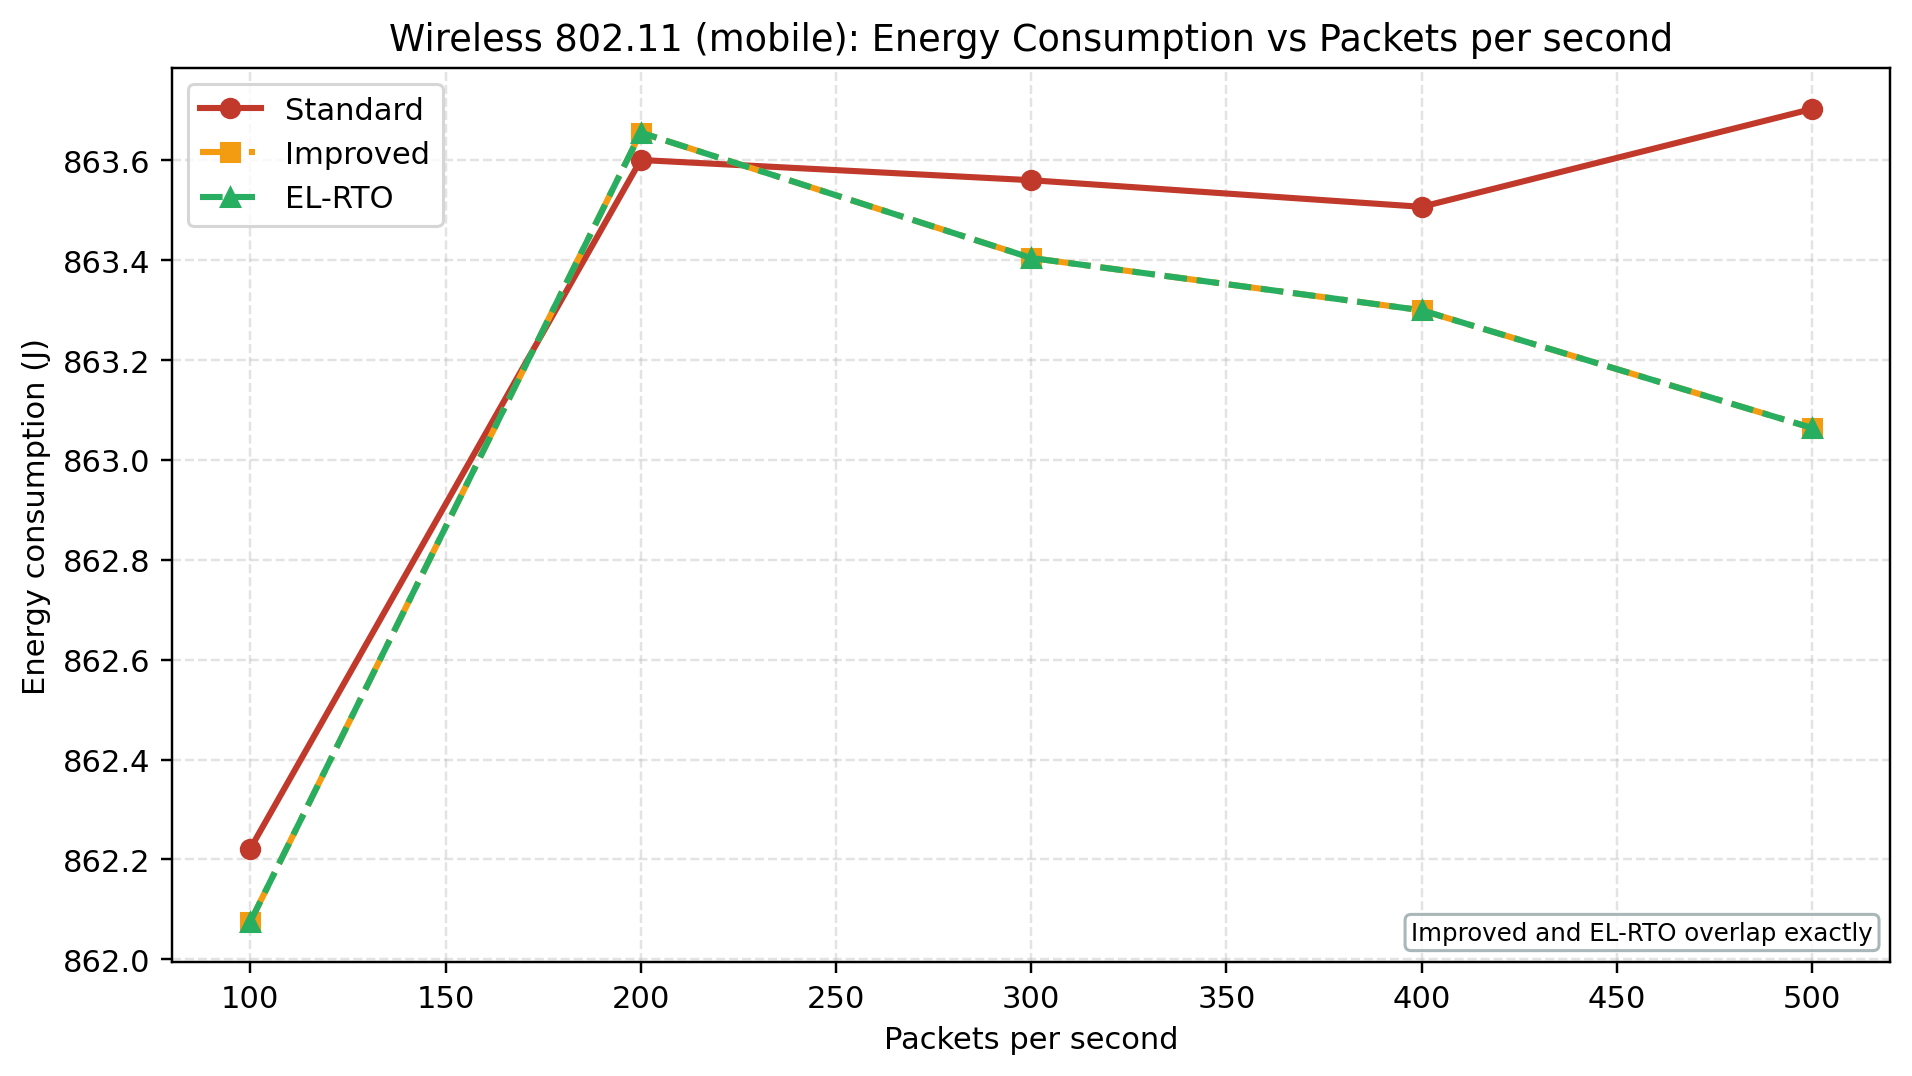
\includegraphics[width=0.47\linewidth]{2105114_final_submission/wifi_mobile/student2105114_wifi_mobile_10s_plots/wifi-mobile_pps_energyJ.png}
\end{frame}

\begin{frame}{Wi-Fi Mobile: Speed Sweep}
  \centering
  \begin{tabular}{cc}
    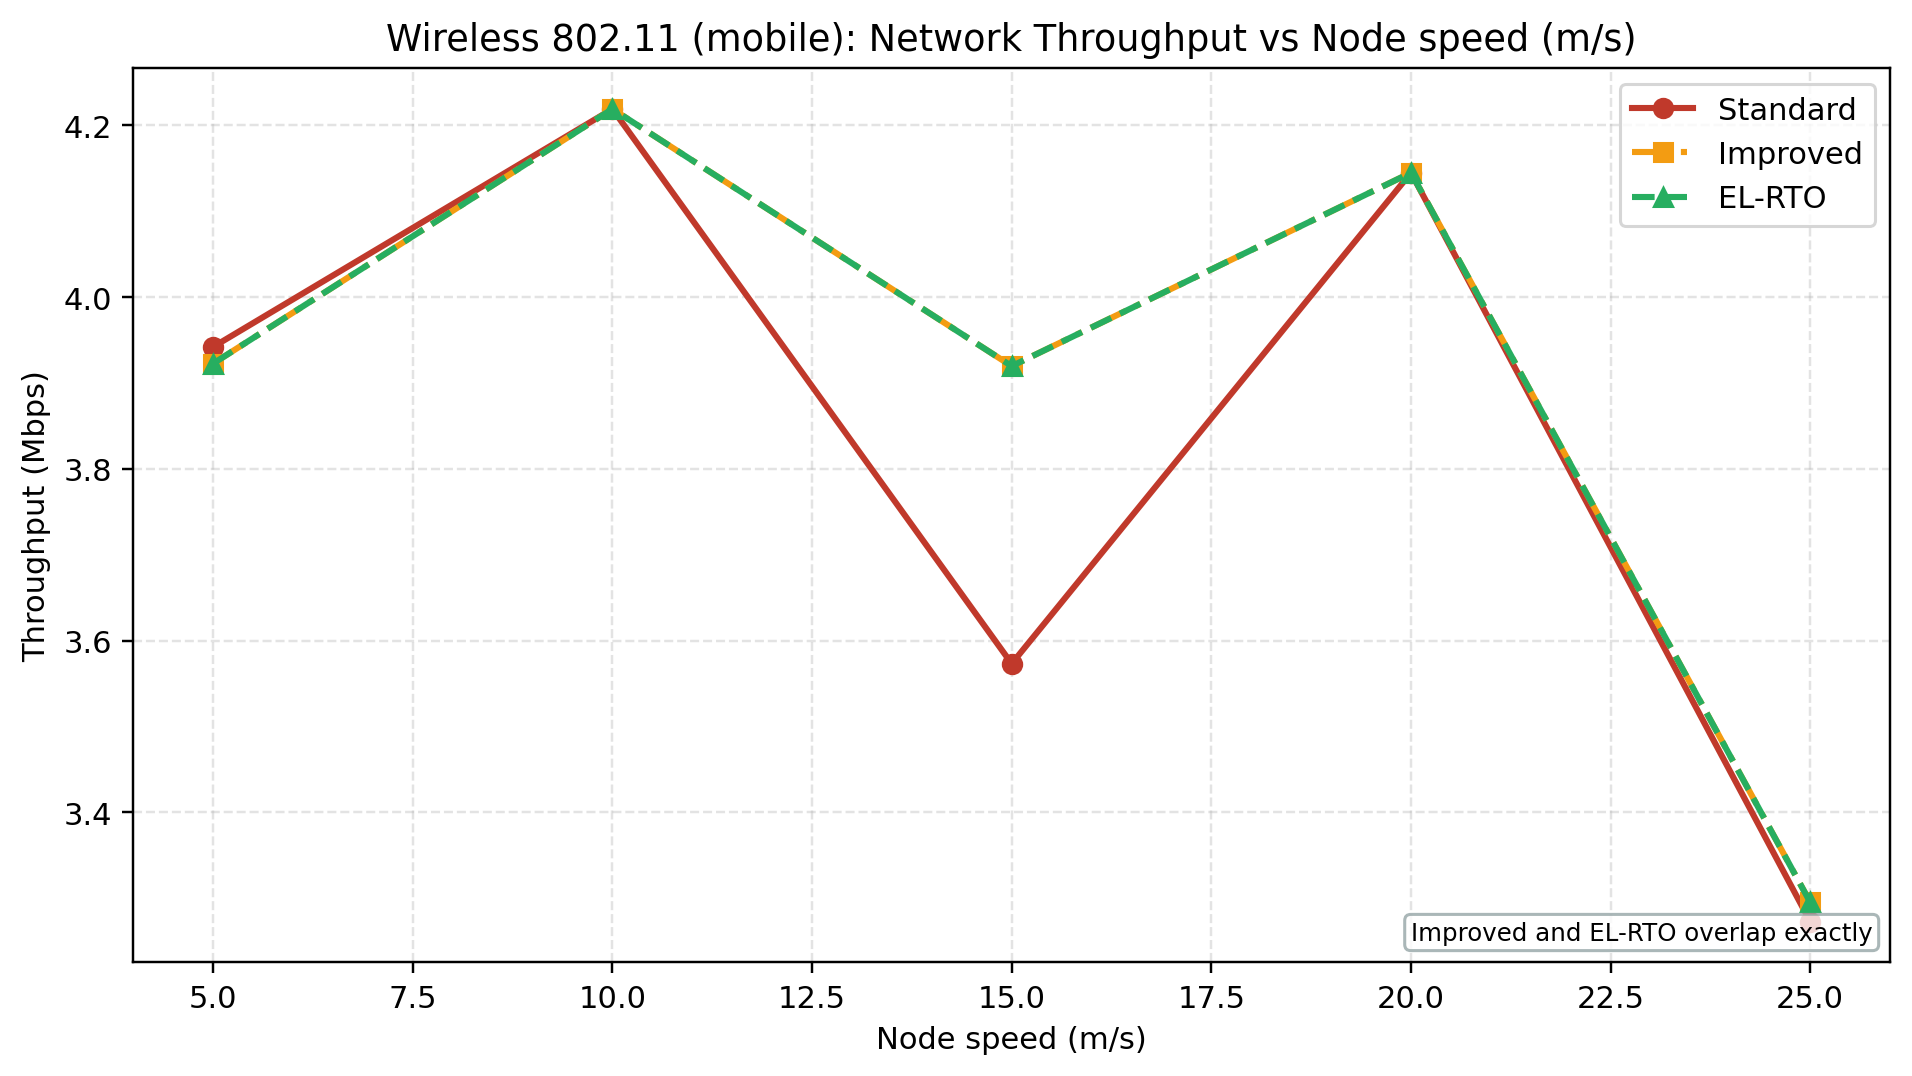
\includegraphics[width=0.47\linewidth]{2105114_final_submission/wifi_mobile/student2105114_wifi_mobile_10s_plots/wifi-mobile_speed_throughputMbps.png} &
    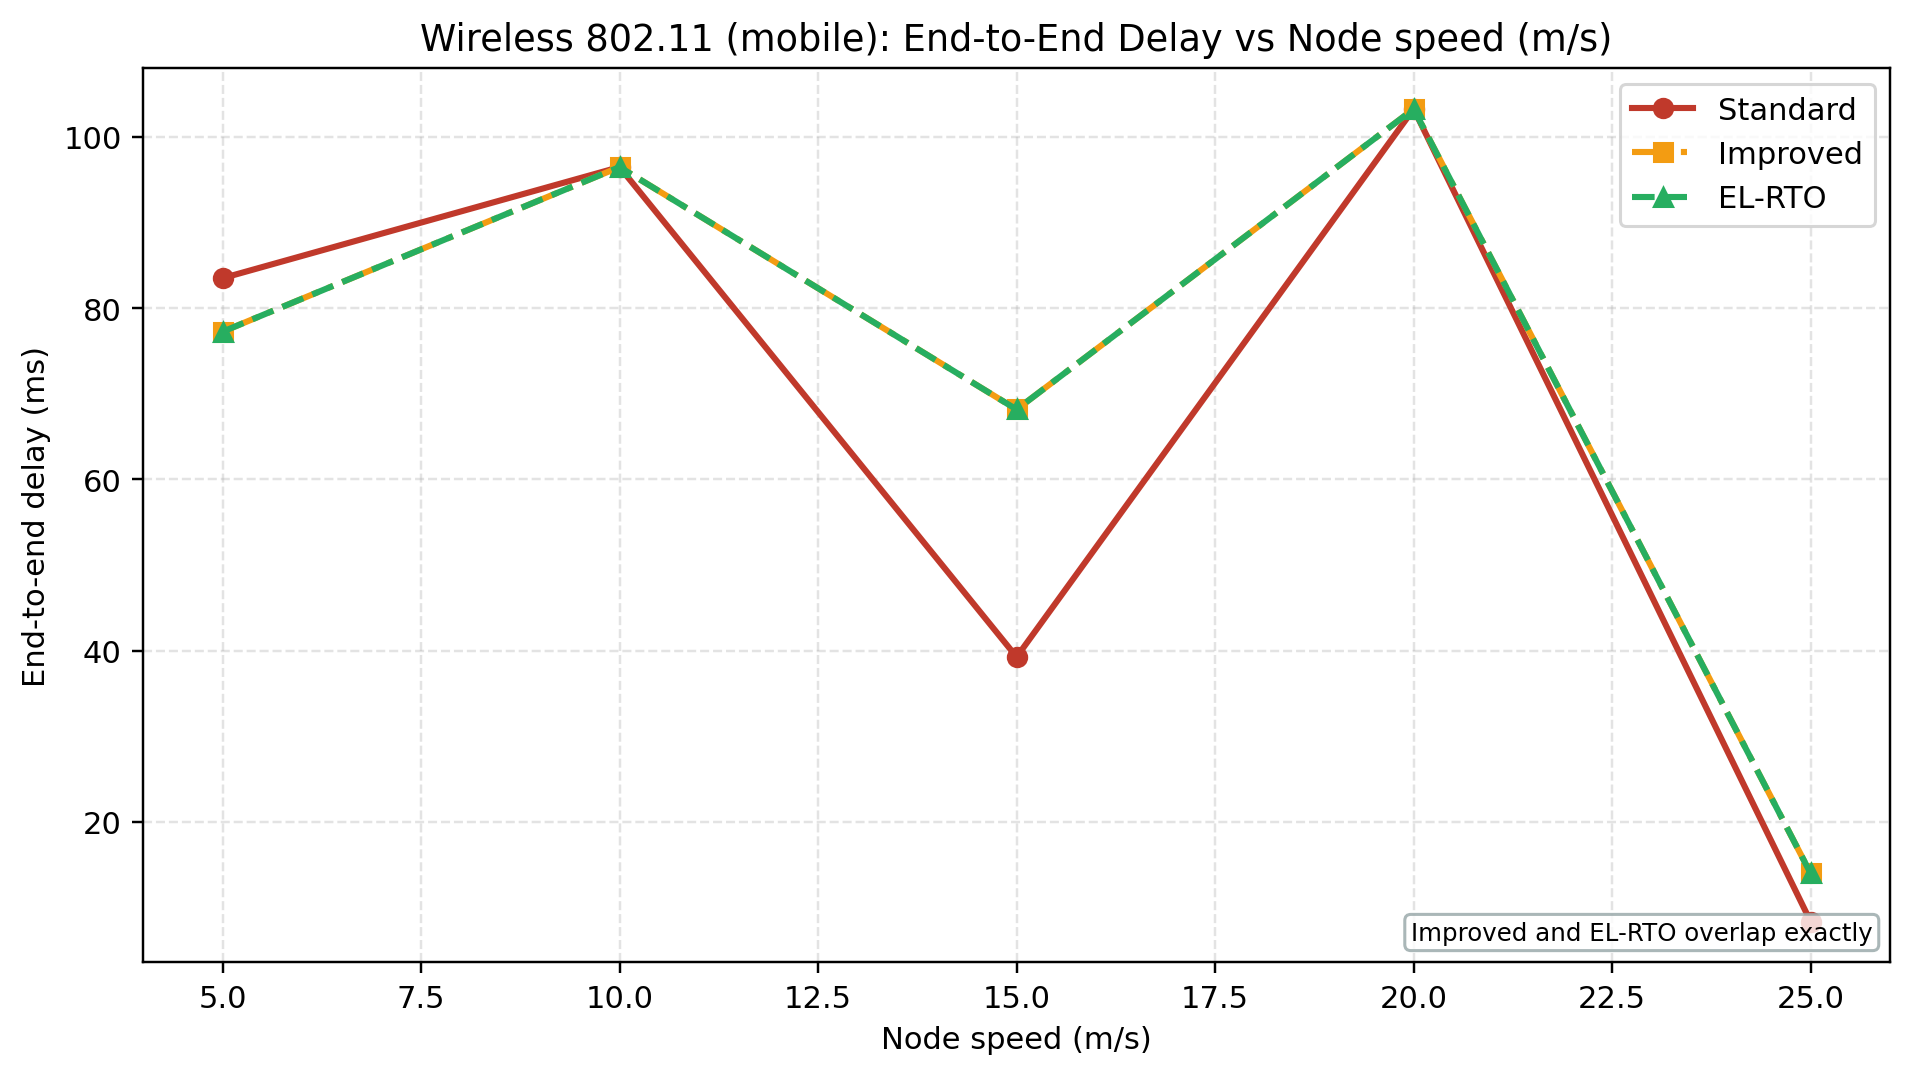
\includegraphics[width=0.47\linewidth]{2105114_final_submission/wifi_mobile/student2105114_wifi_mobile_10s_plots/wifi-mobile_speed_averageDelayMs.png} \\
    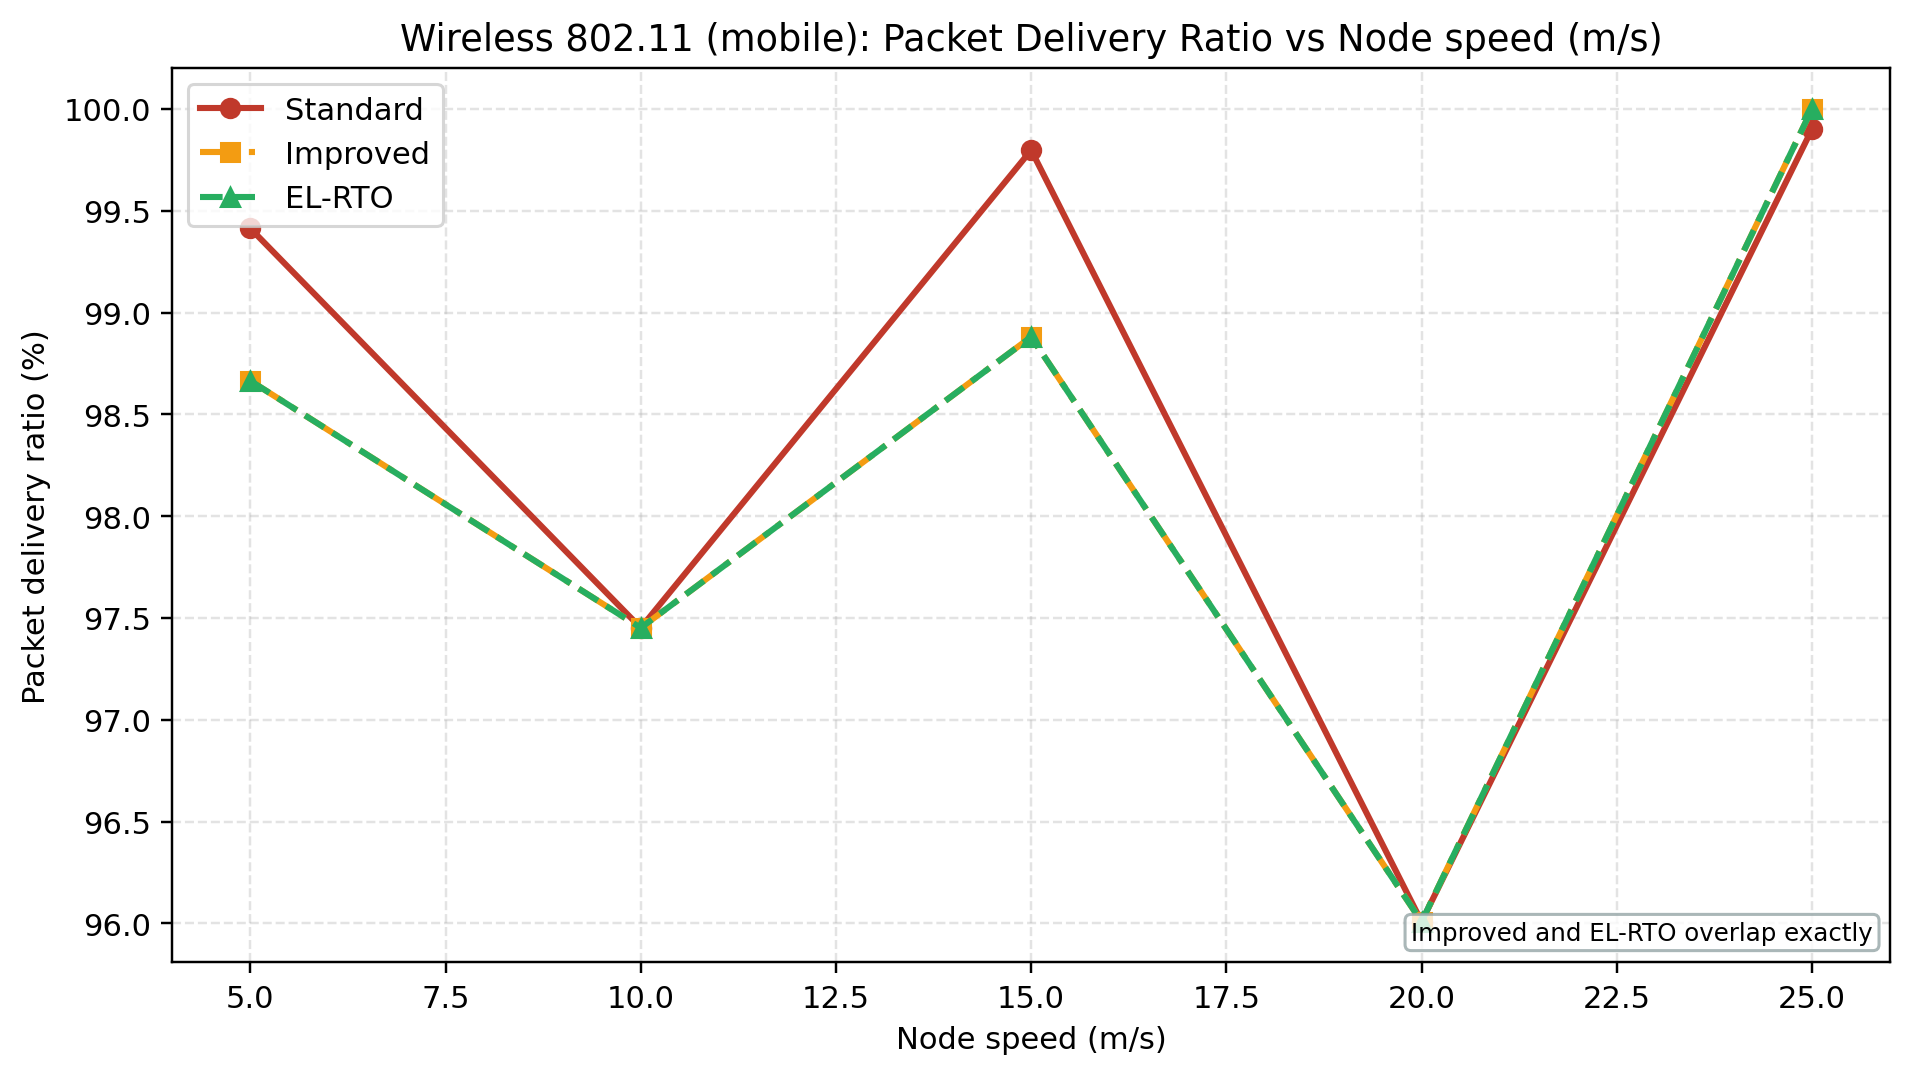
\includegraphics[width=0.47\linewidth]{2105114_final_submission/wifi_mobile/student2105114_wifi_mobile_10s_plots/wifi-mobile_speed_pdrPct.png} &
    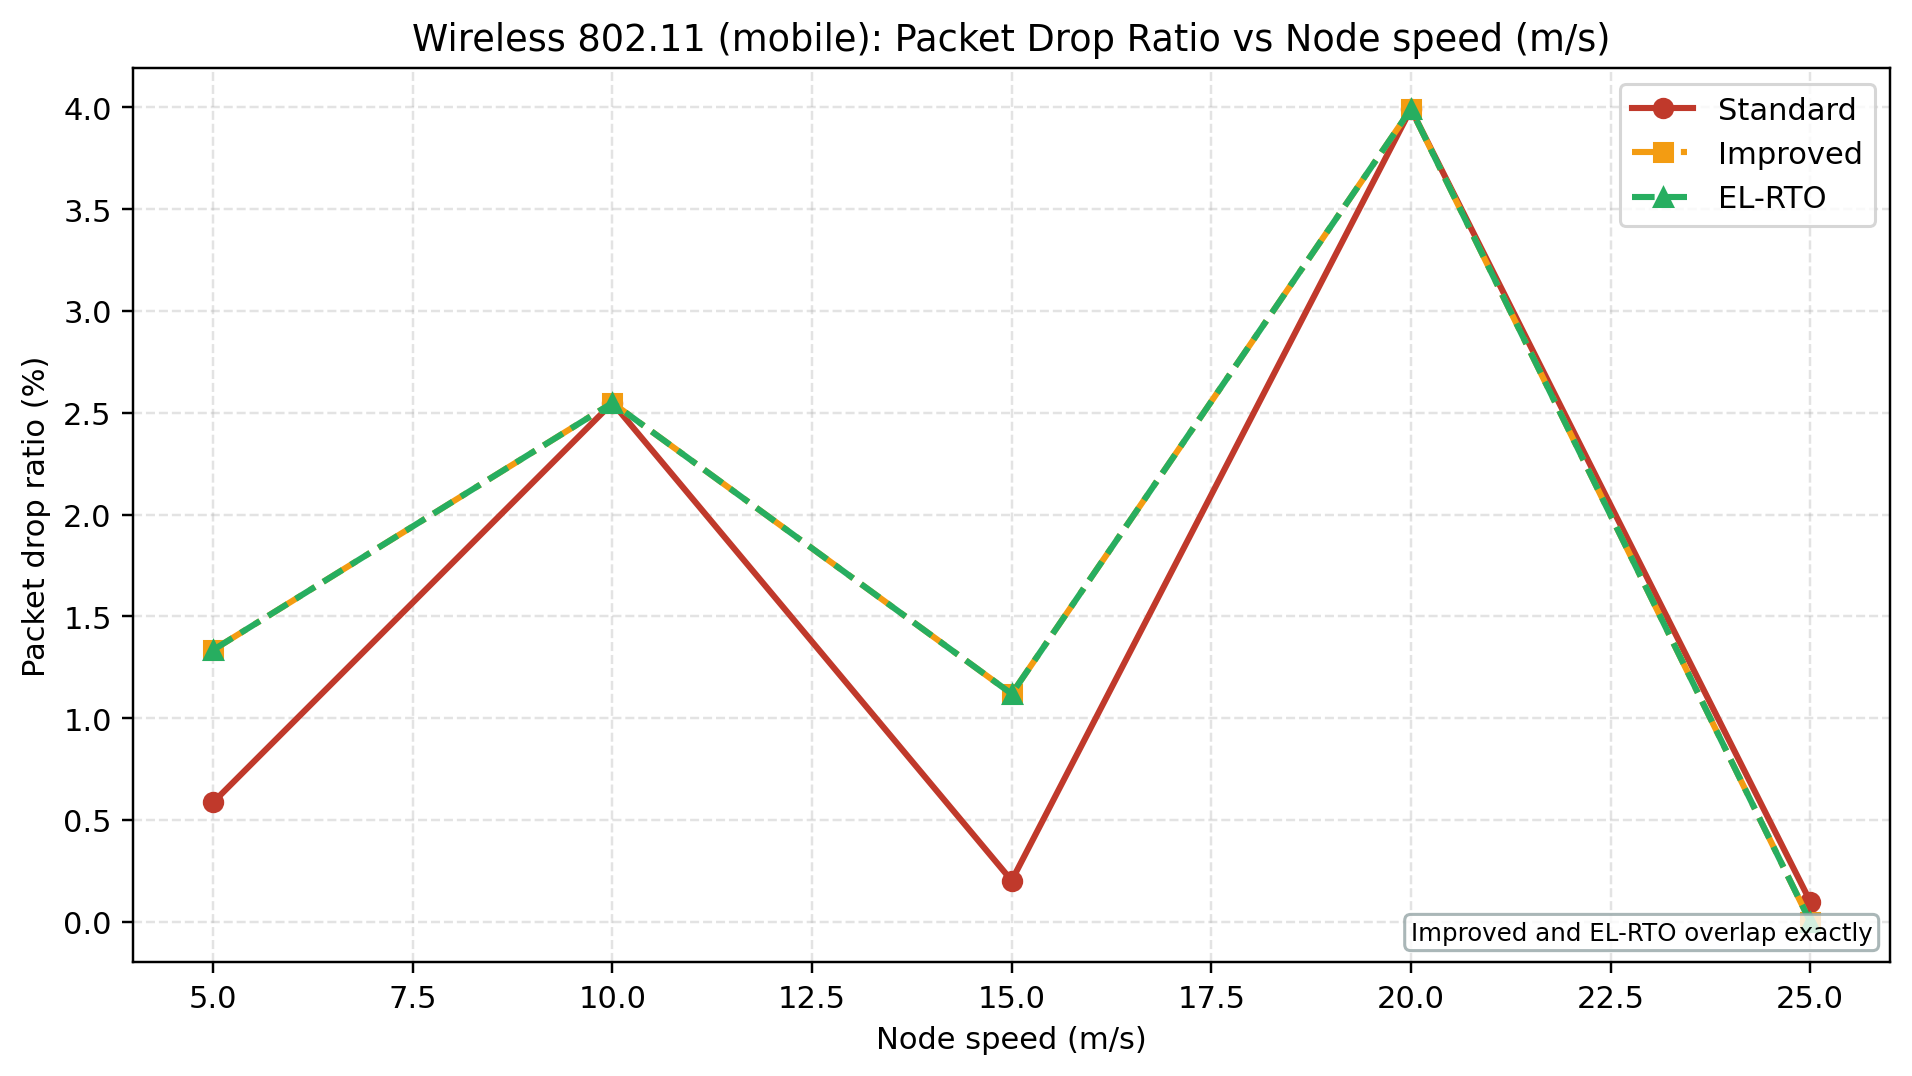
\includegraphics[width=0.47\linewidth]{2105114_final_submission/wifi_mobile/student2105114_wifi_mobile_10s_plots/wifi-mobile_speed_dropRatioPct.png}
  \end{tabular}

  \vspace{0.15cm}
  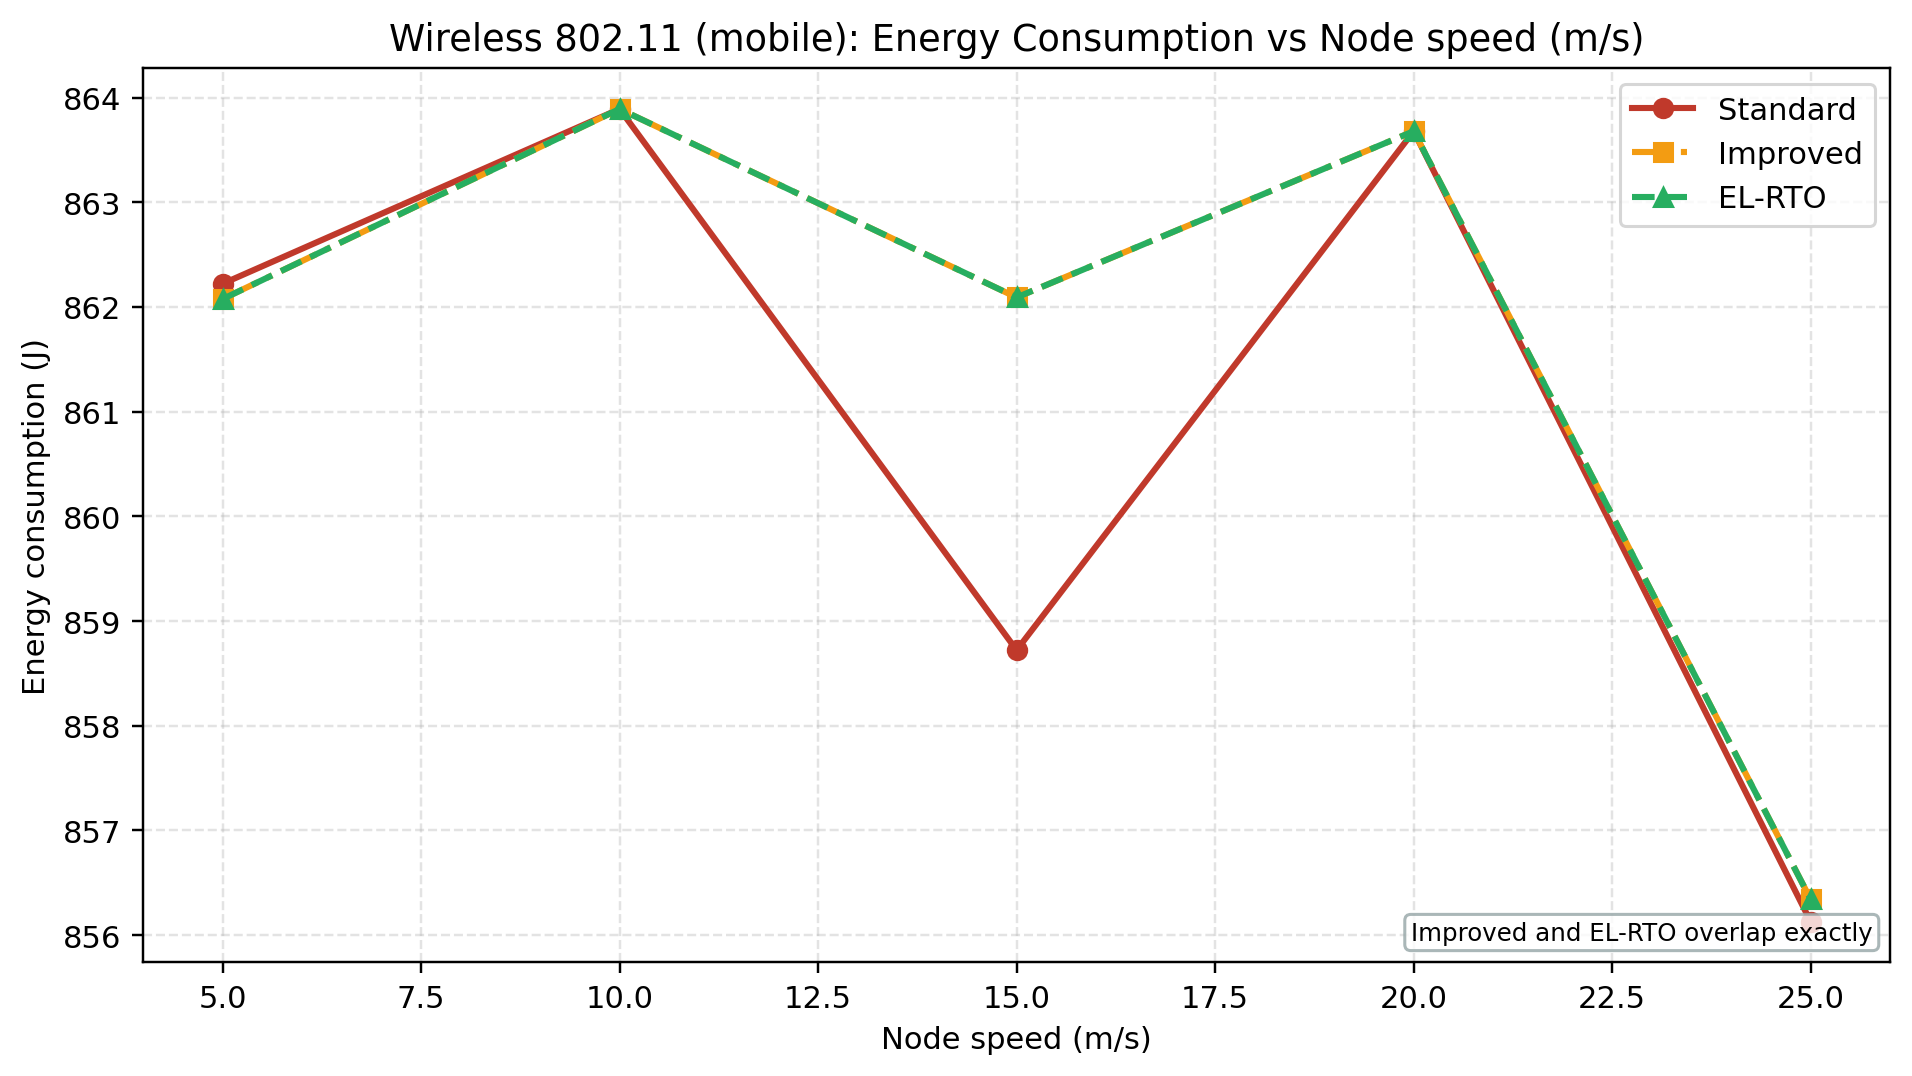
\includegraphics[width=0.47\linewidth]{2105114_final_submission/wifi_mobile/student2105114_wifi_mobile_10s_plots/wifi-mobile_speed_energyJ.png}
\end{frame}

\begin{frame}{LR-WPAN Mobile: Node Sweep}
  \centering
  \begin{tabular}{cc}
    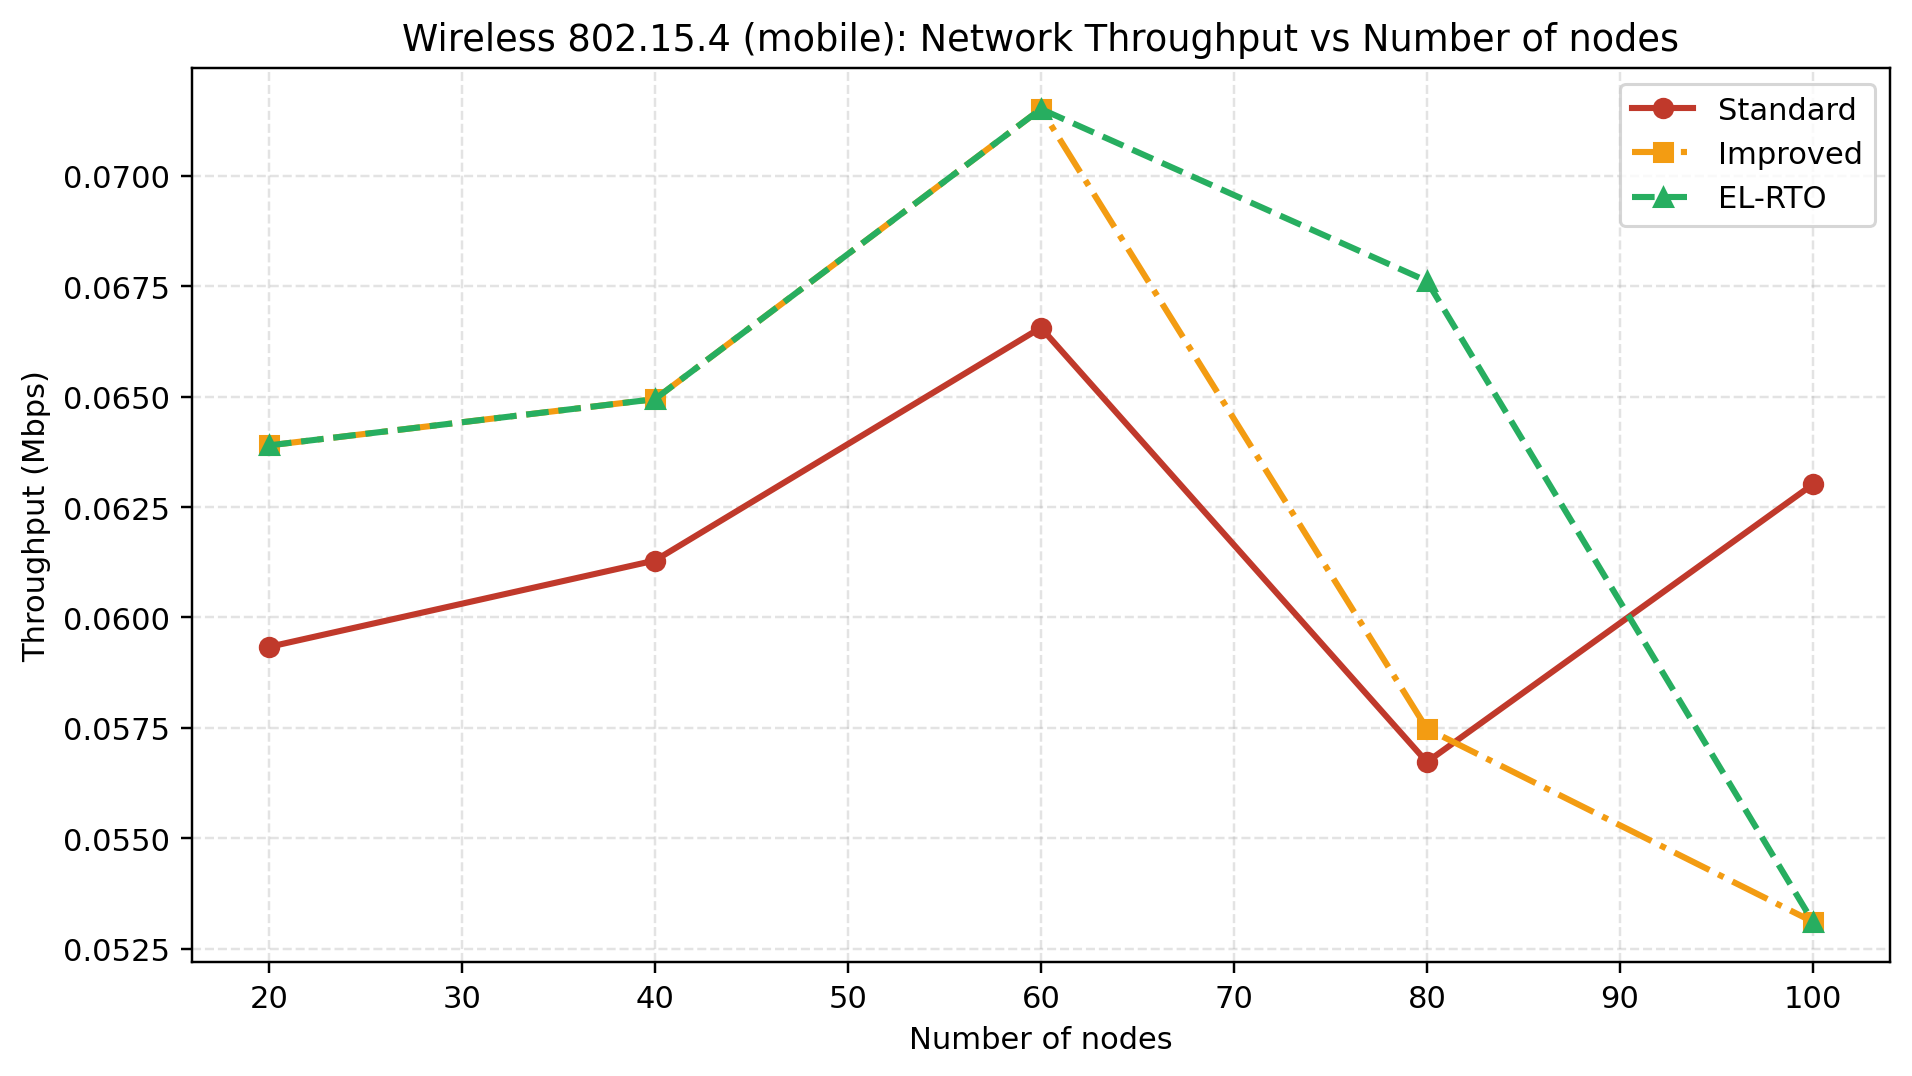
\includegraphics[width=0.47\linewidth]{2105114_final_submission/lrwpan_mobile/student2105114_lrwpan_mobile_10s_plots/lrwpan-mobile_nodes_throughputMbps.png} &
    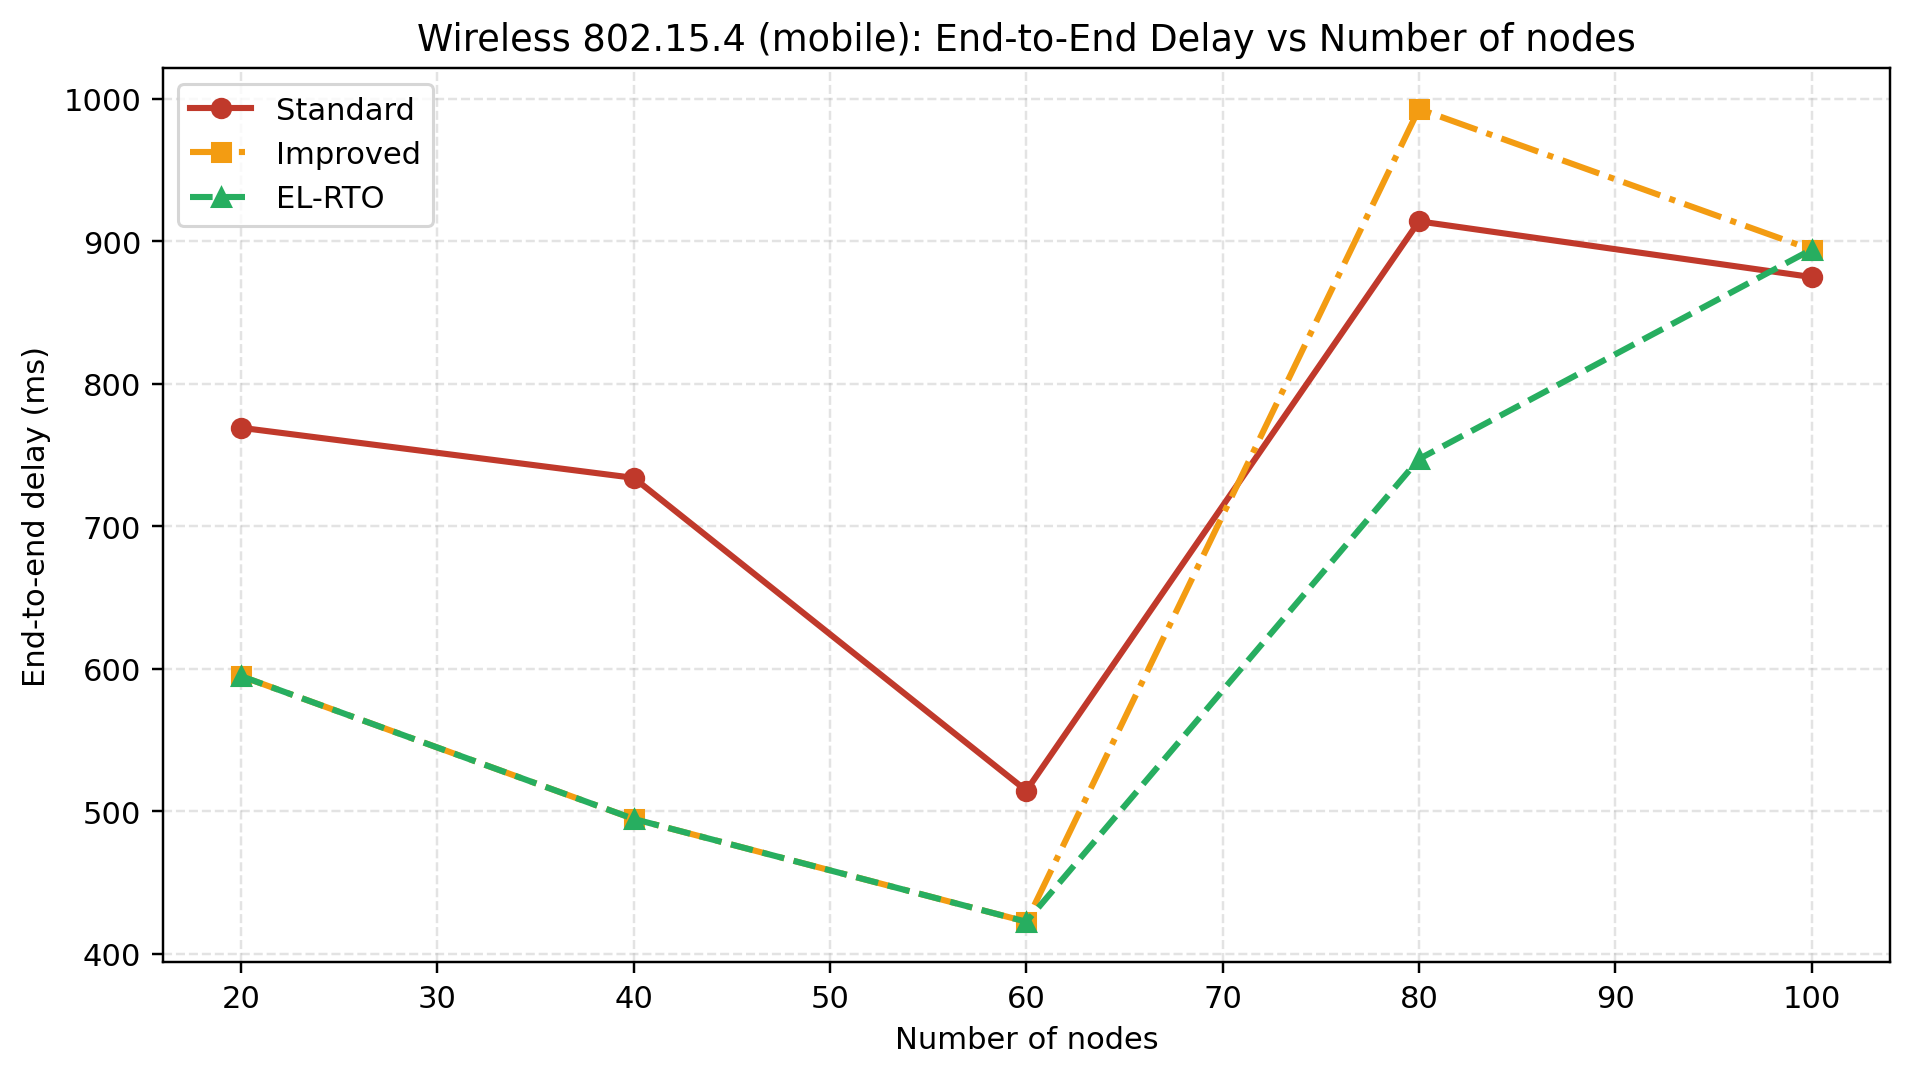
\includegraphics[width=0.47\linewidth]{2105114_final_submission/lrwpan_mobile/student2105114_lrwpan_mobile_10s_plots/lrwpan-mobile_nodes_averageDelayMs.png} \\
    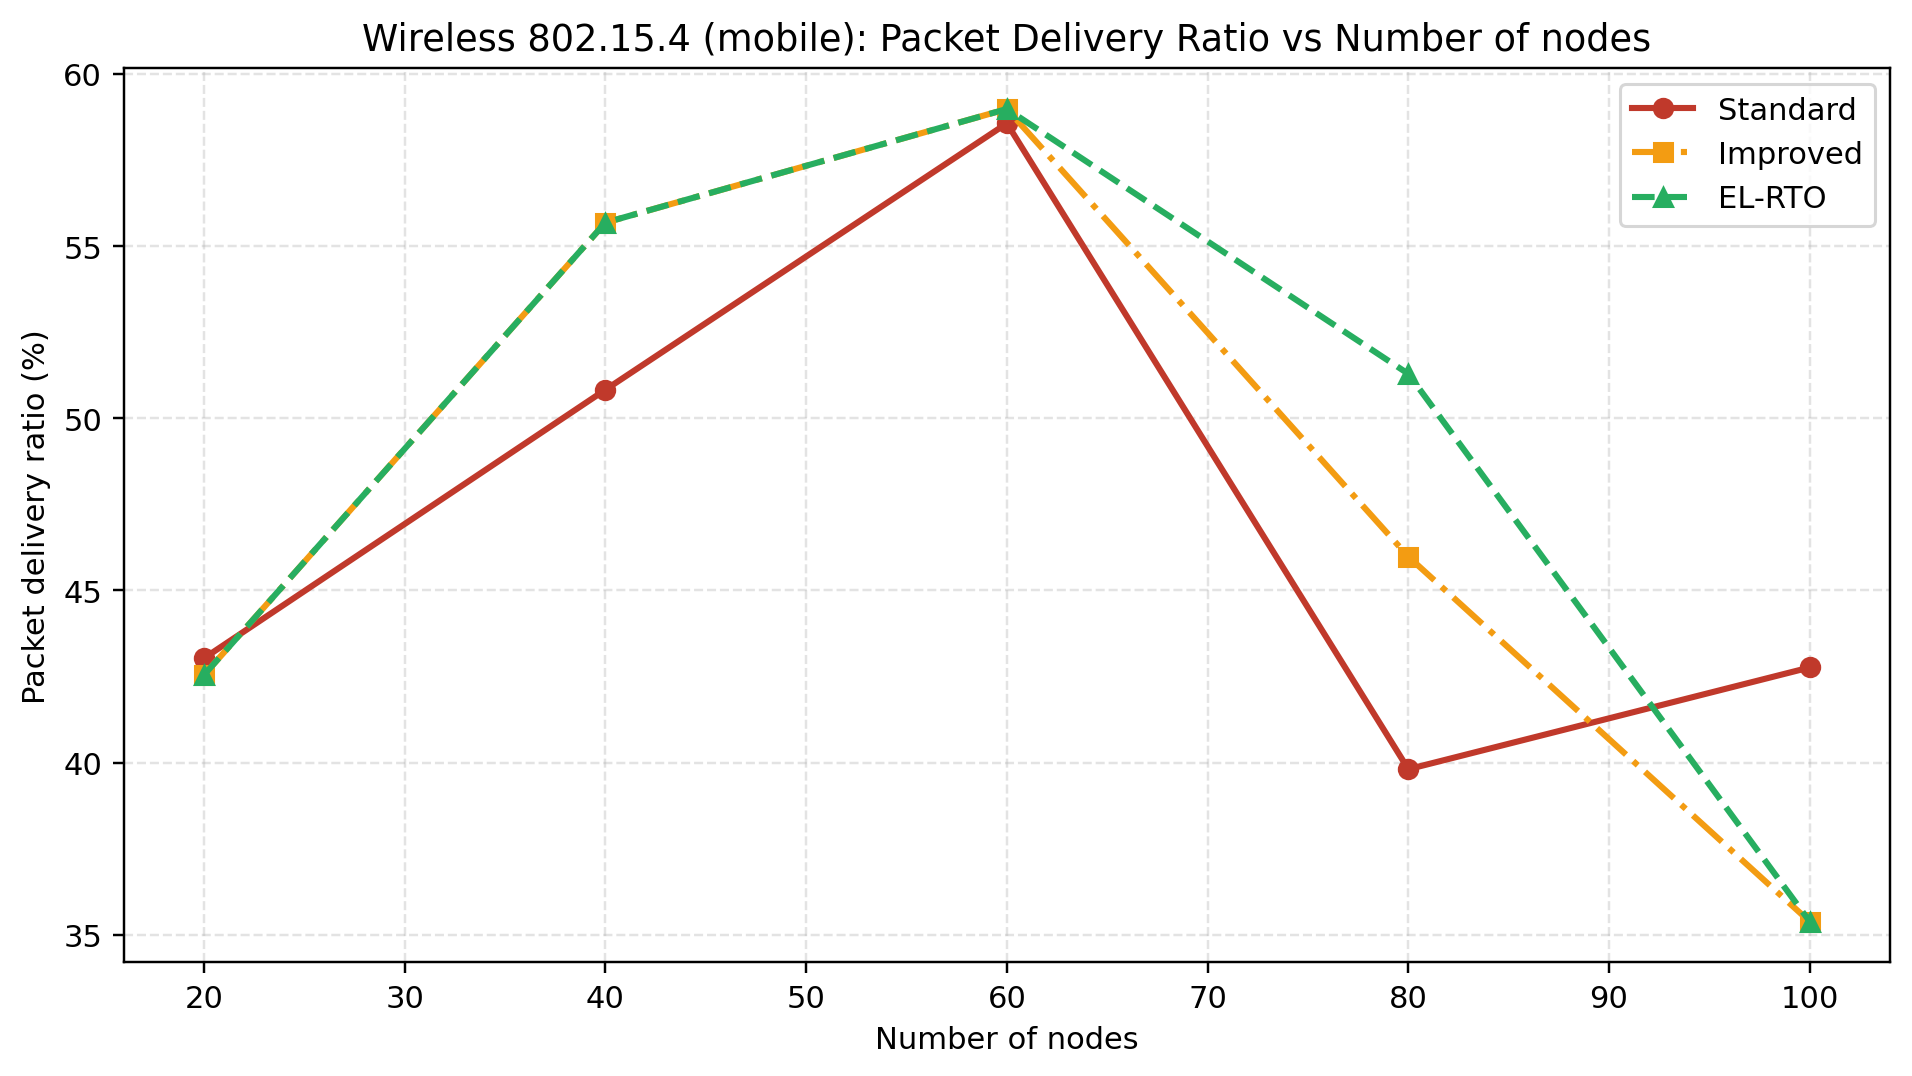
\includegraphics[width=0.47\linewidth]{2105114_final_submission/lrwpan_mobile/student2105114_lrwpan_mobile_10s_plots/lrwpan-mobile_nodes_pdrPct.png} &
    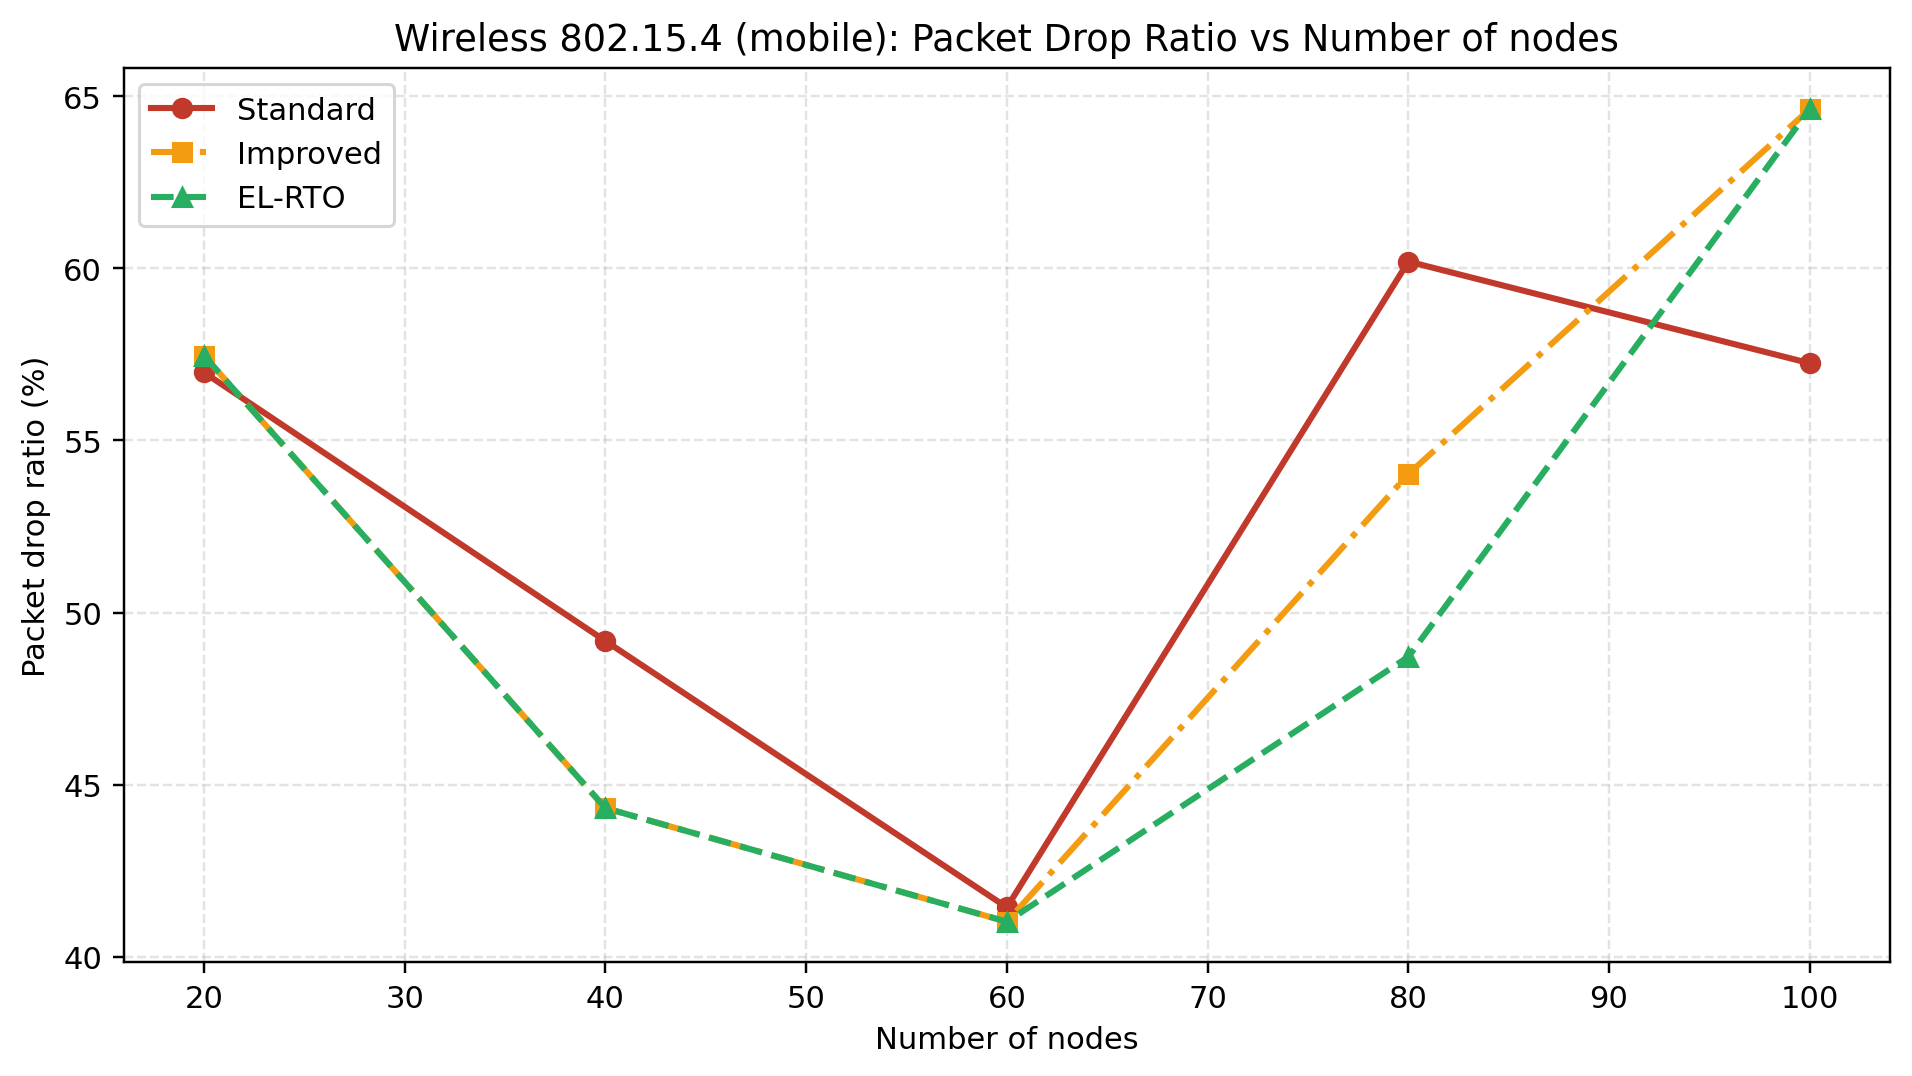
\includegraphics[width=0.47\linewidth]{2105114_final_submission/lrwpan_mobile/student2105114_lrwpan_mobile_10s_plots/lrwpan-mobile_nodes_dropRatioPct.png}
  \end{tabular}

  \vspace{0.15cm}
  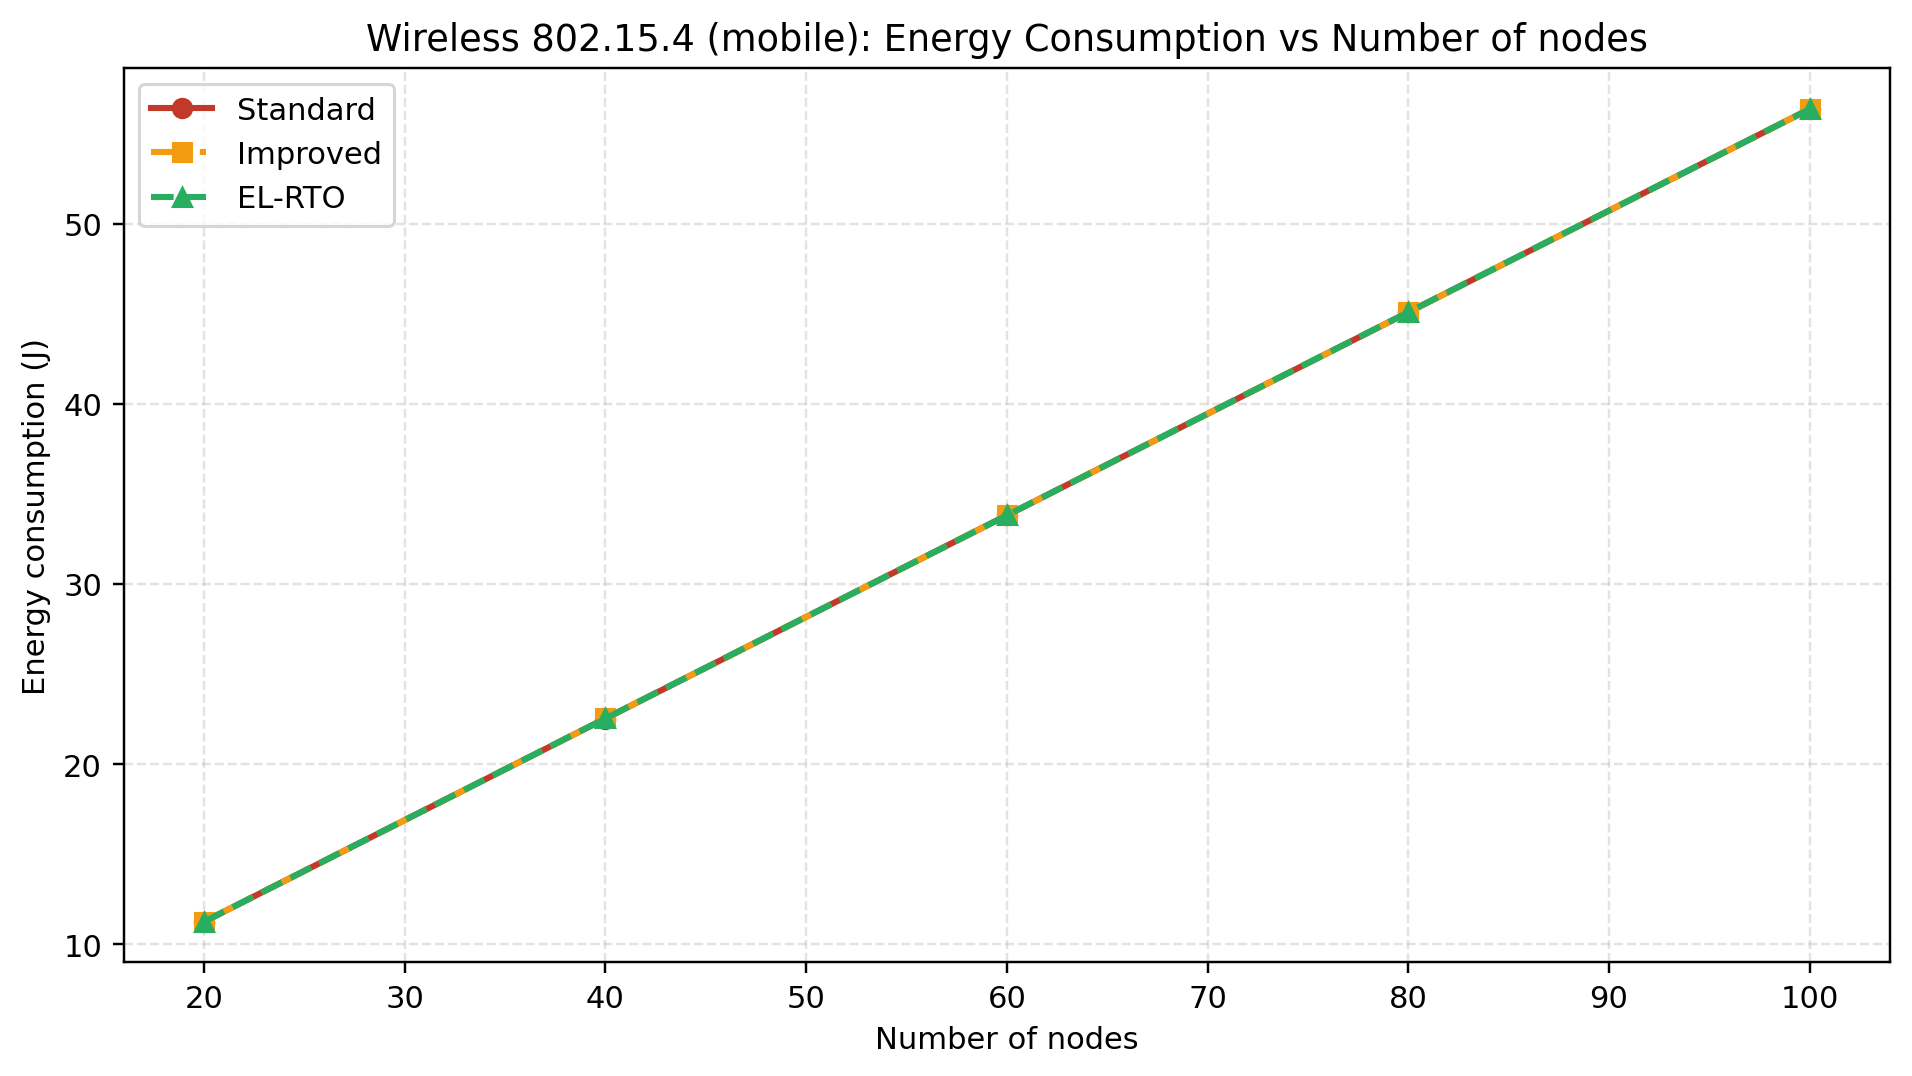
\includegraphics[width=0.47\linewidth]{2105114_final_submission/lrwpan_mobile/student2105114_lrwpan_mobile_10s_plots/lrwpan-mobile_nodes_energyJ.png}
\end{frame}

\begin{frame}{LR-WPAN Mobile: Flow Sweep}
  \centering
  \begin{tabular}{cc}
    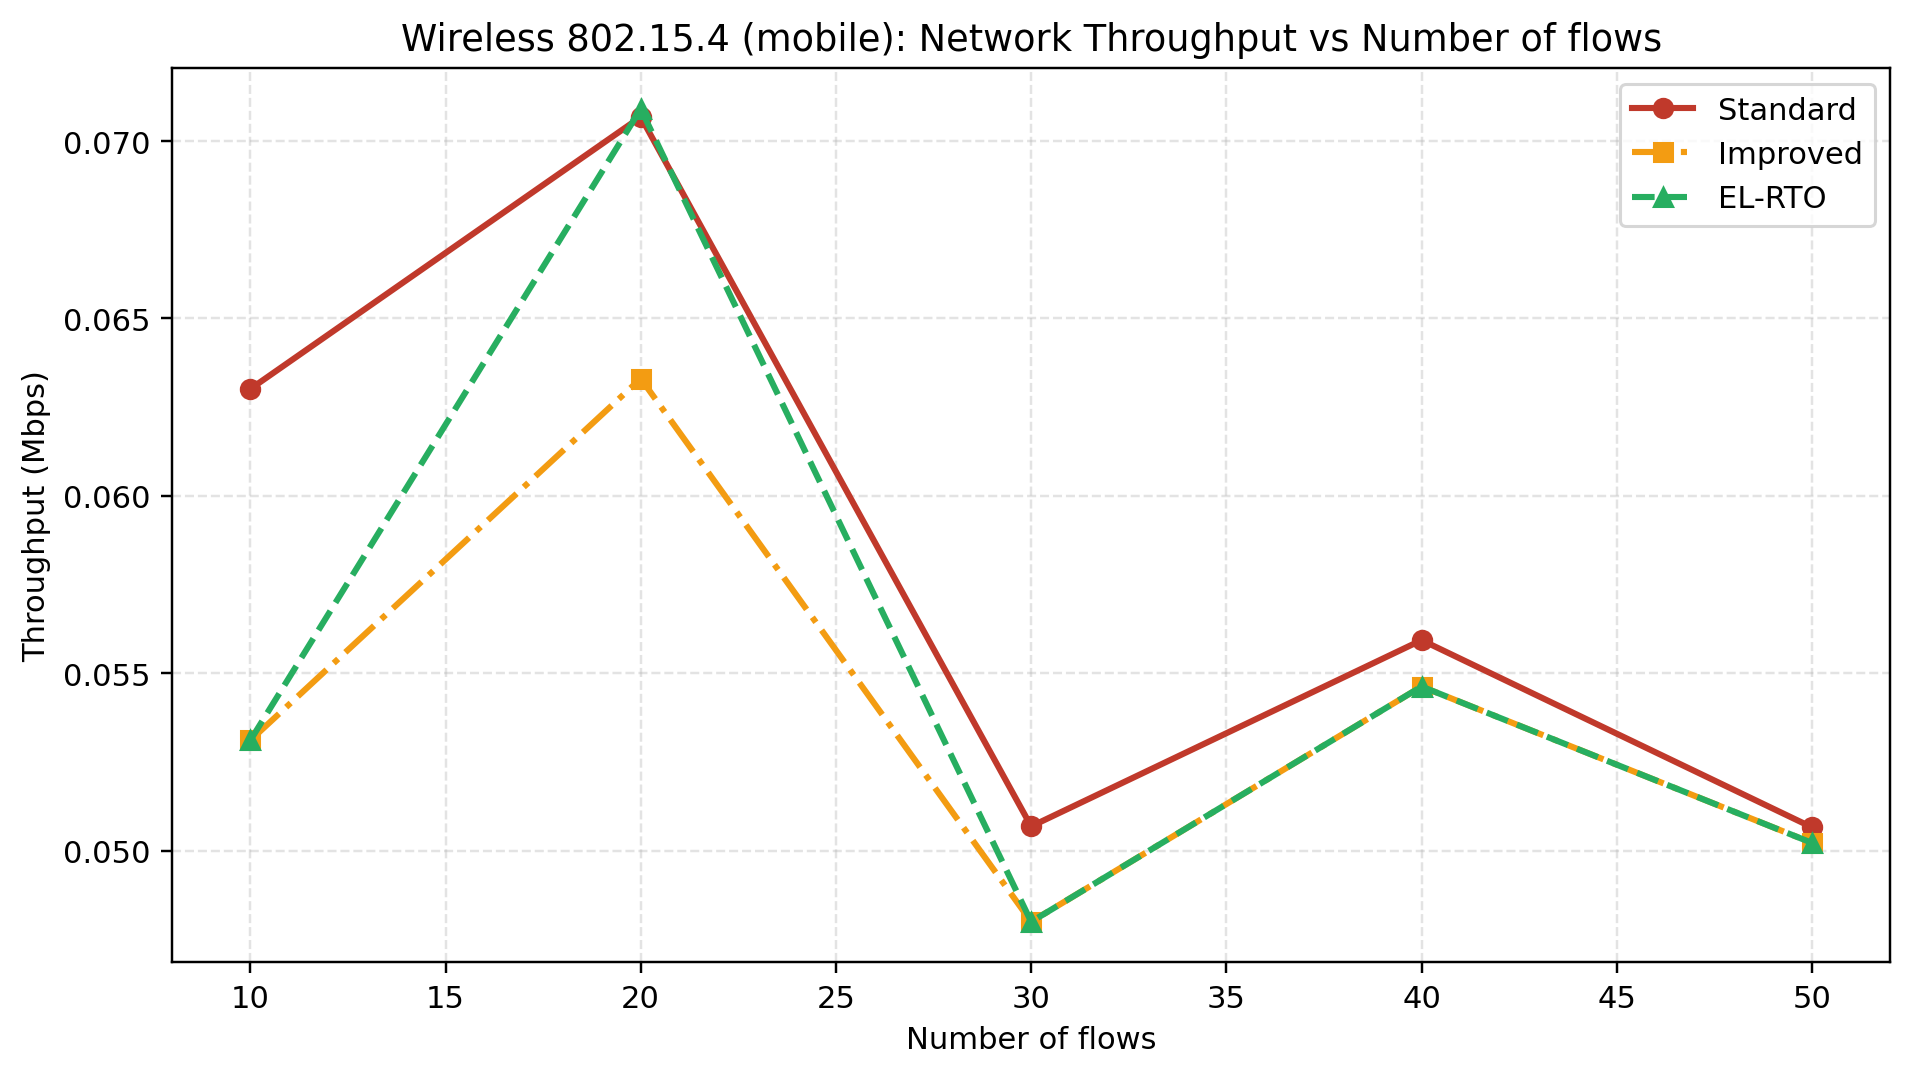
\includegraphics[width=0.47\linewidth]{2105114_final_submission/lrwpan_mobile/student2105114_lrwpan_mobile_10s_plots/lrwpan-mobile_flows_throughputMbps.png} &
    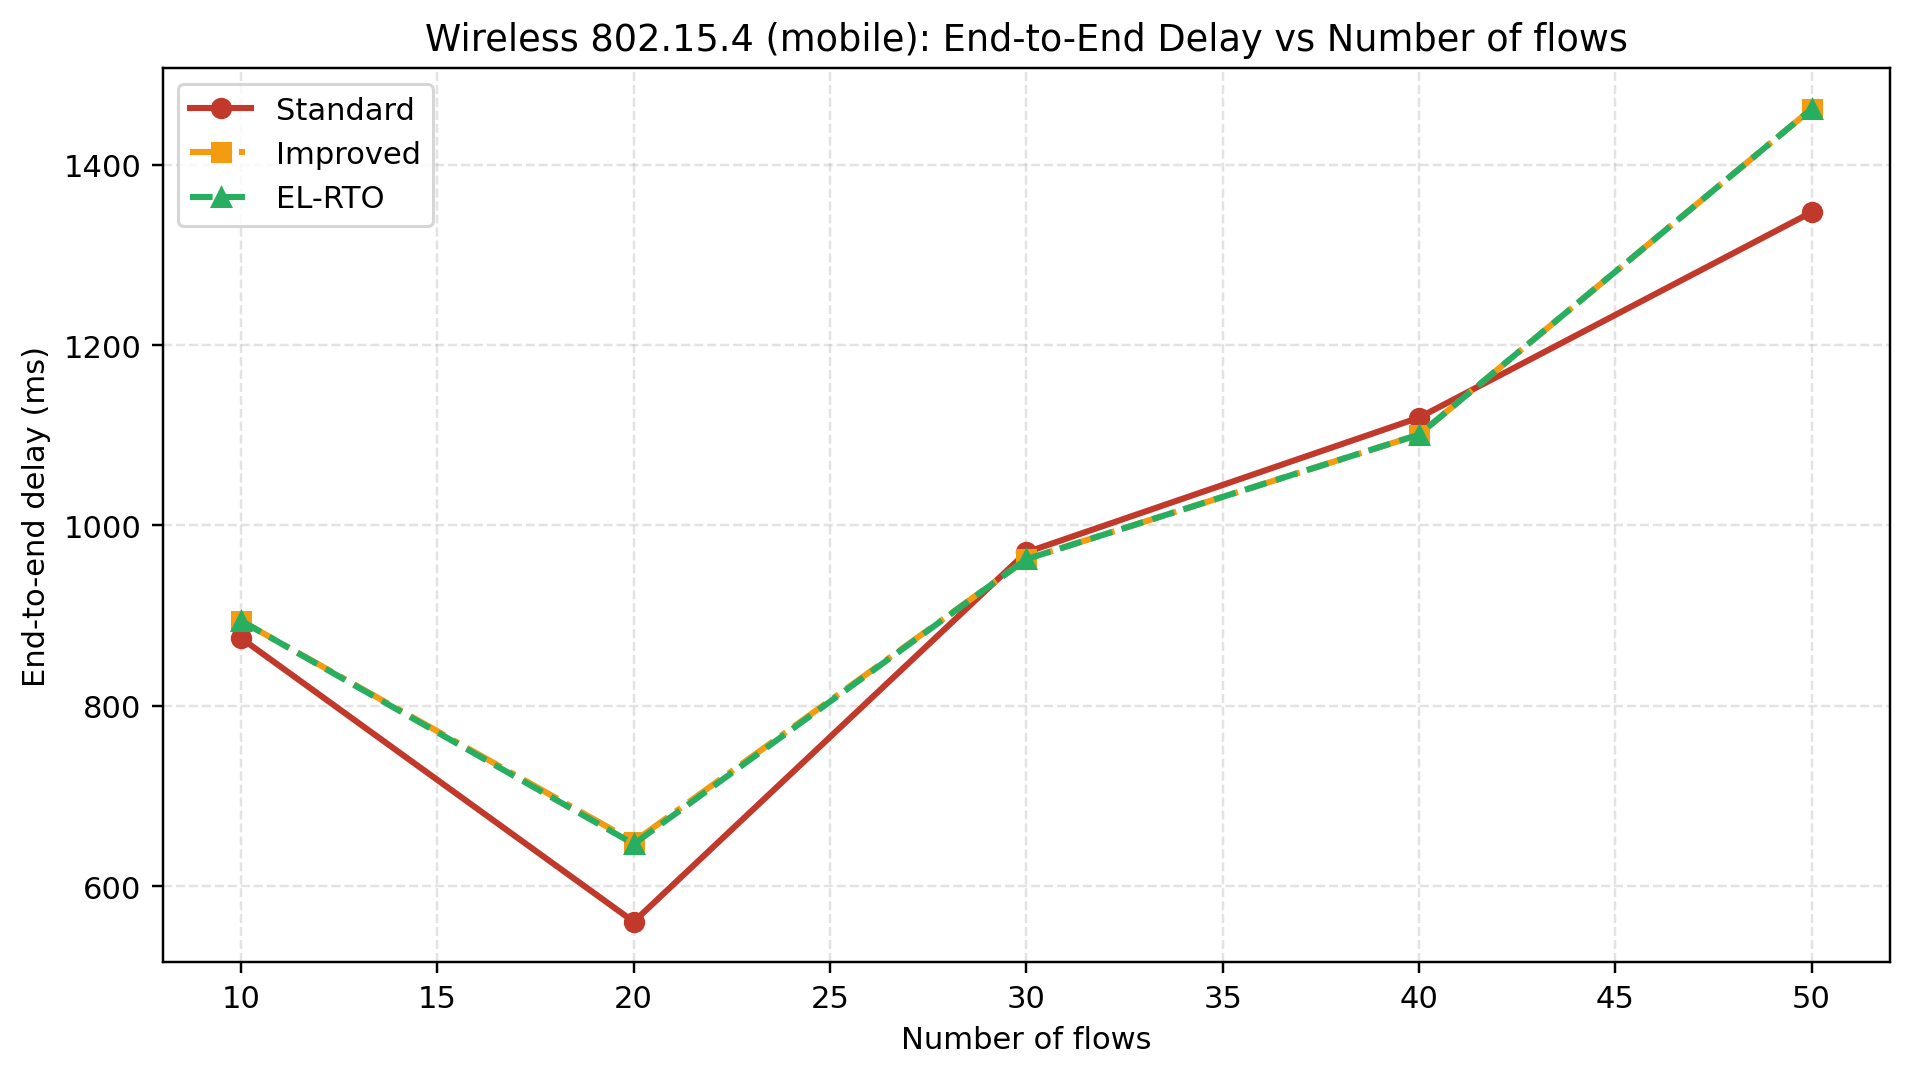
\includegraphics[width=0.47\linewidth]{2105114_final_submission/lrwpan_mobile/student2105114_lrwpan_mobile_10s_plots/lrwpan-mobile_flows_averageDelayMs.png} \\
    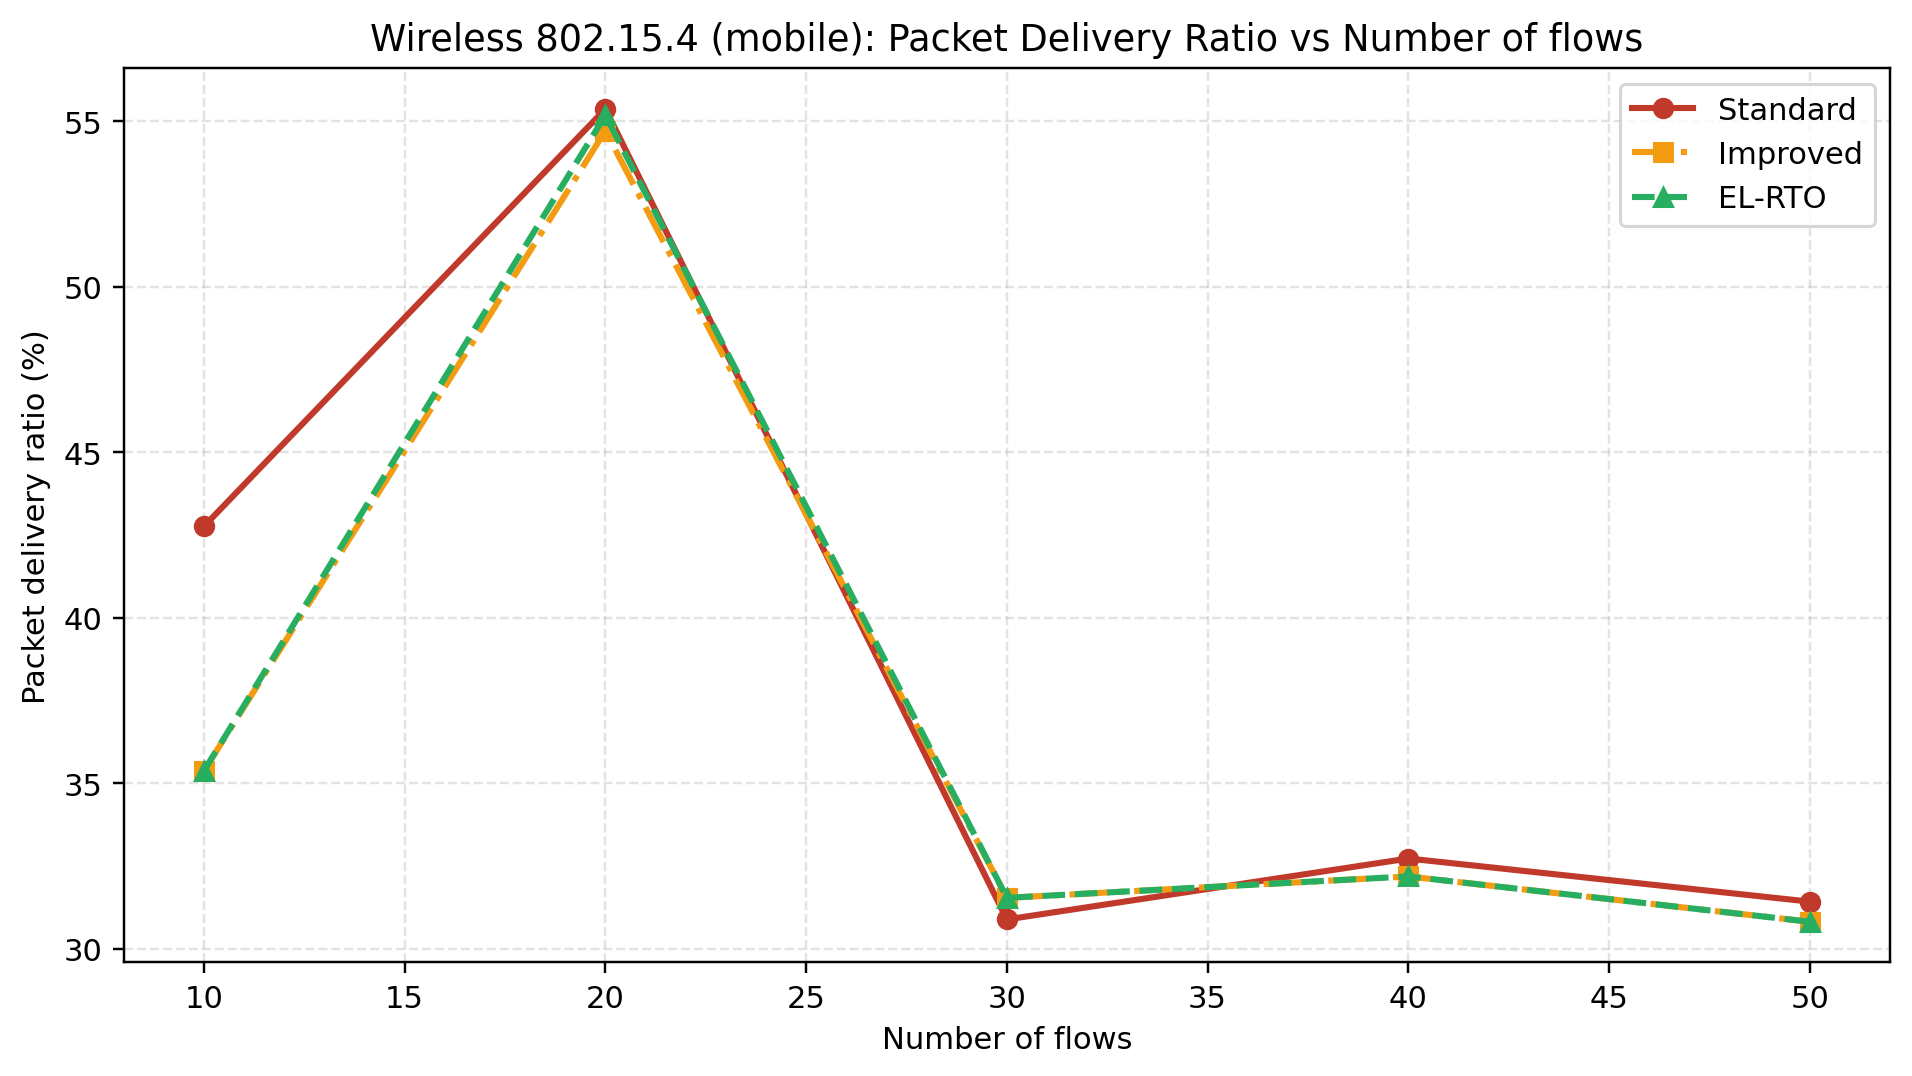
\includegraphics[width=0.47\linewidth]{2105114_final_submission/lrwpan_mobile/student2105114_lrwpan_mobile_10s_plots/lrwpan-mobile_flows_pdrPct.png} &
    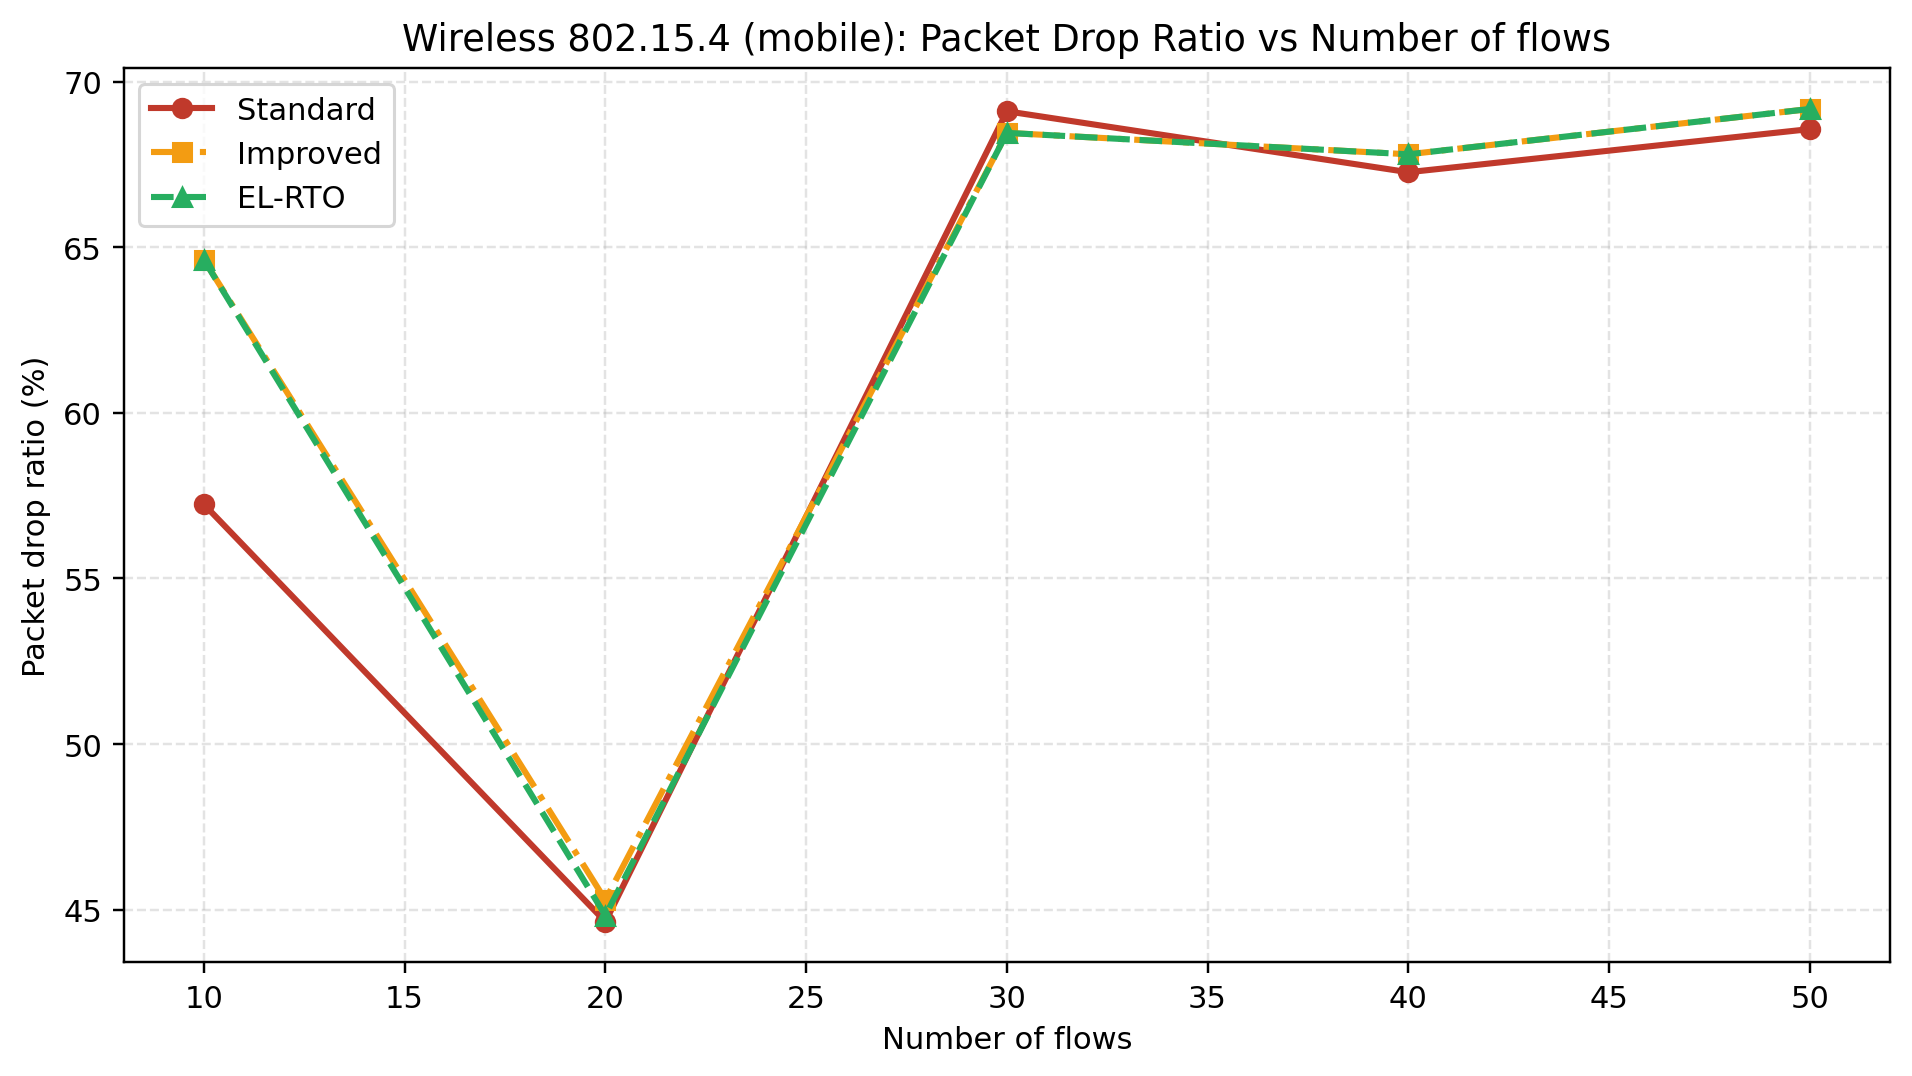
\includegraphics[width=0.47\linewidth]{2105114_final_submission/lrwpan_mobile/student2105114_lrwpan_mobile_10s_plots/lrwpan-mobile_flows_dropRatioPct.png}
  \end{tabular}

  \vspace{0.15cm}
  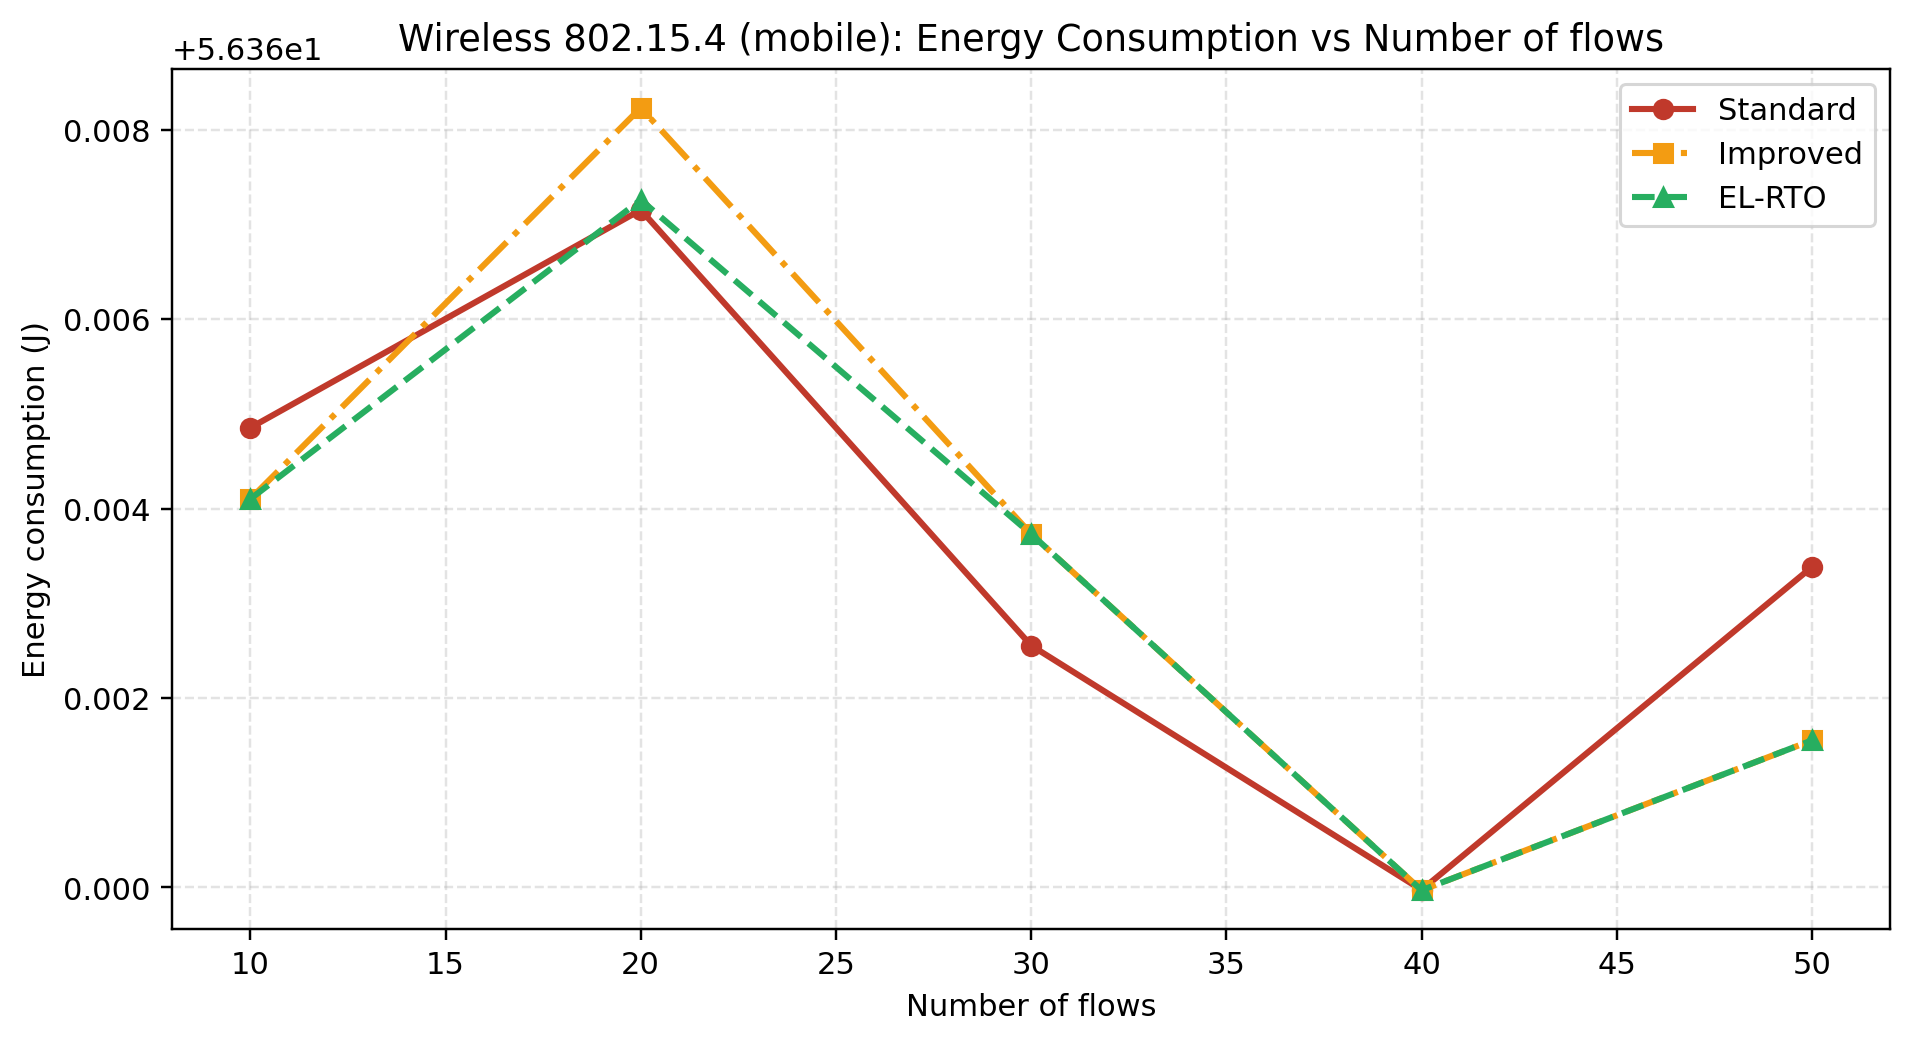
\includegraphics[width=0.47\linewidth]{2105114_final_submission/lrwpan_mobile/student2105114_lrwpan_mobile_10s_plots/lrwpan-mobile_flows_energyJ.png}
\end{frame}

\begin{frame}{LR-WPAN Mobile: Packet-Rate Sweep}
  \centering
  \begin{tabular}{cc}
    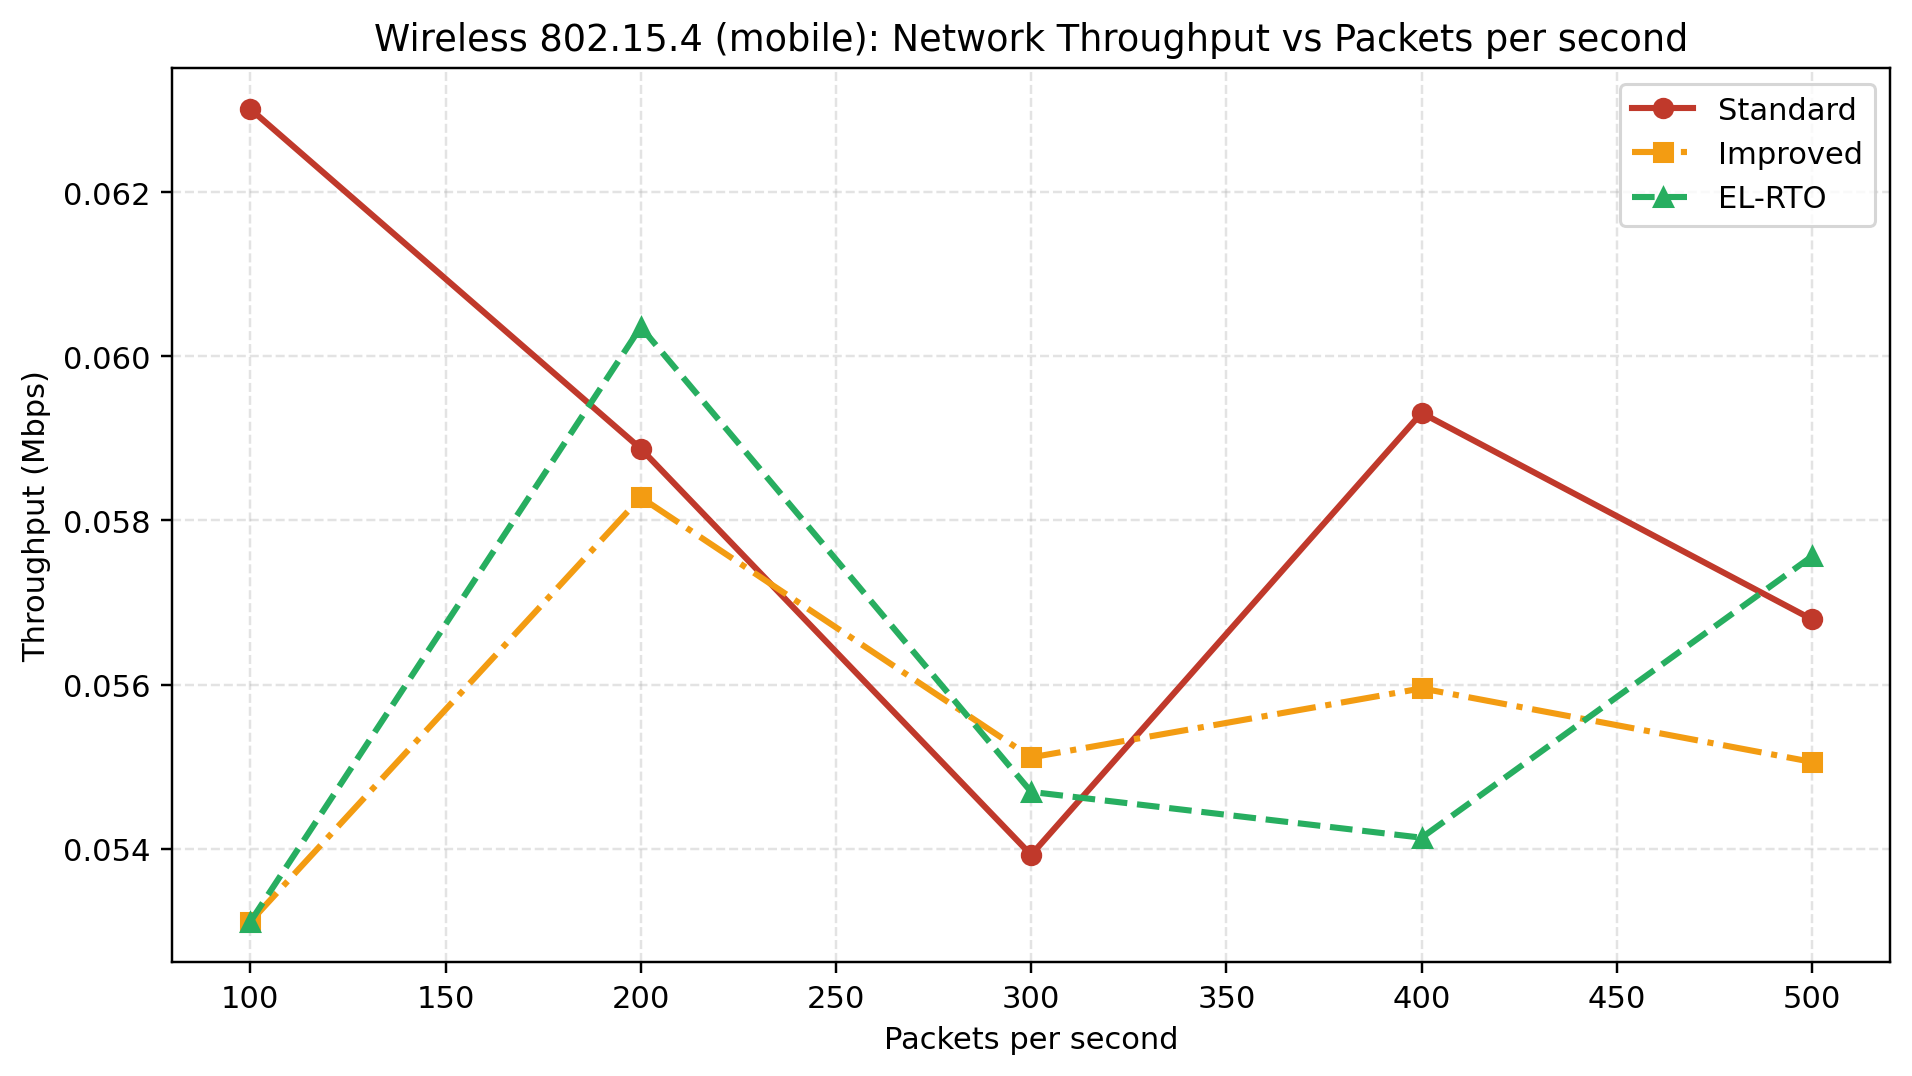
\includegraphics[width=0.47\linewidth]{2105114_final_submission/lrwpan_mobile/student2105114_lrwpan_mobile_10s_plots/lrwpan-mobile_pps_throughputMbps.png} &
    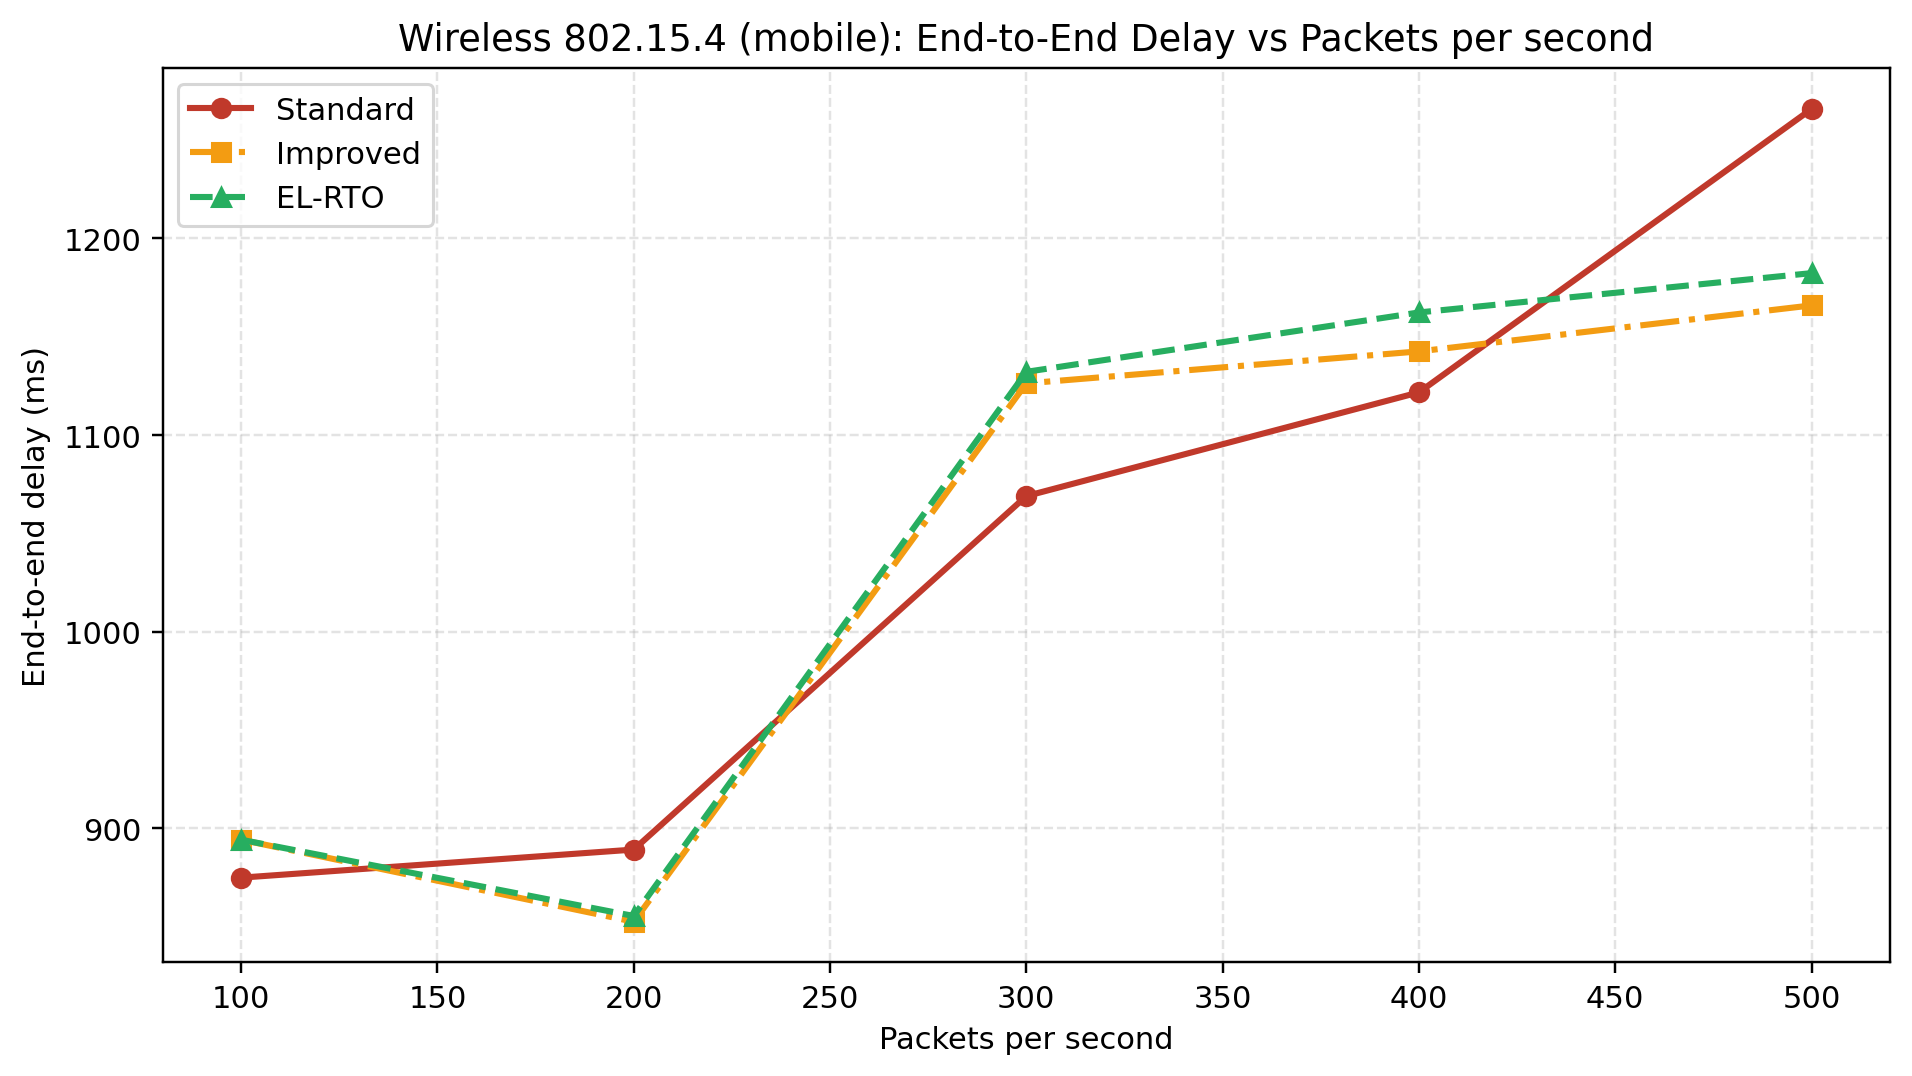
\includegraphics[width=0.47\linewidth]{2105114_final_submission/lrwpan_mobile/student2105114_lrwpan_mobile_10s_plots/lrwpan-mobile_pps_averageDelayMs.png} \\
    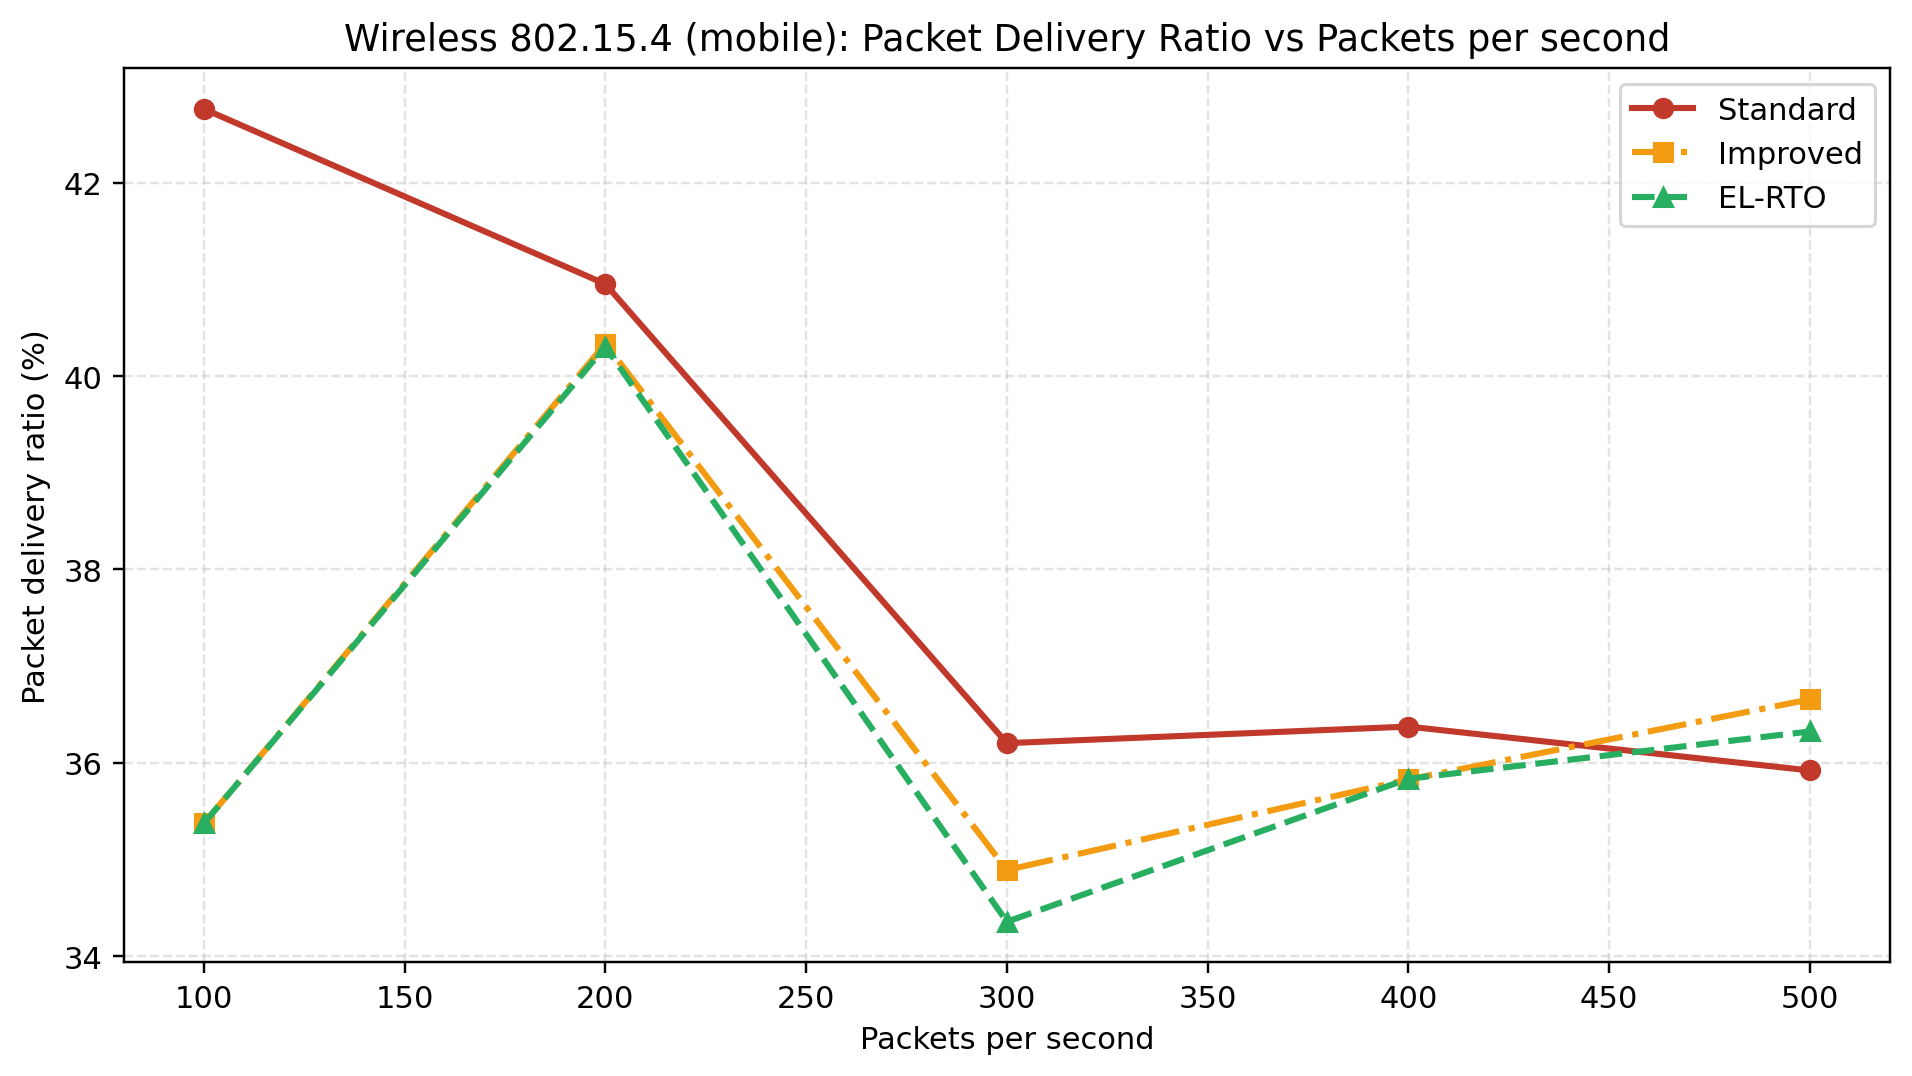
\includegraphics[width=0.47\linewidth]{2105114_final_submission/lrwpan_mobile/student2105114_lrwpan_mobile_10s_plots/lrwpan-mobile_pps_pdrPct.png} &
    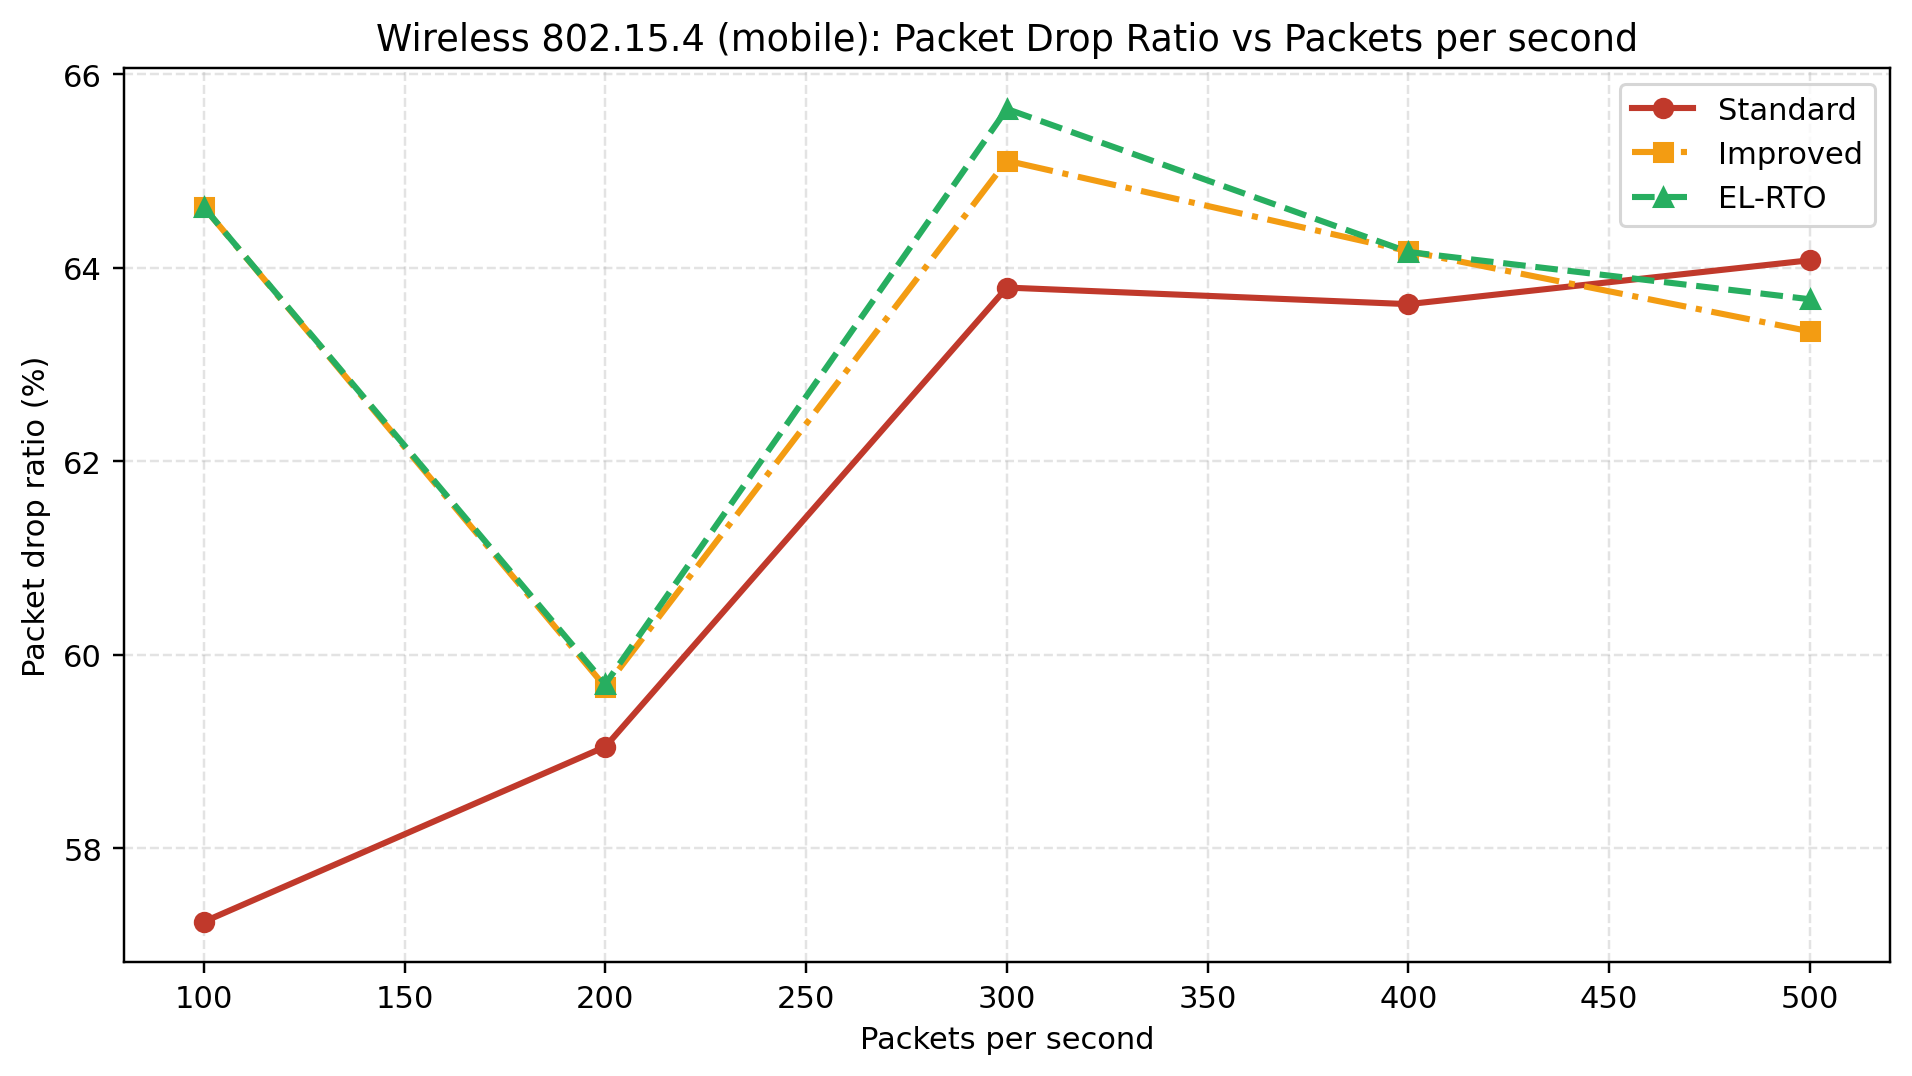
\includegraphics[width=0.47\linewidth]{2105114_final_submission/lrwpan_mobile/student2105114_lrwpan_mobile_10s_plots/lrwpan-mobile_pps_dropRatioPct.png}
  \end{tabular}

  \vspace{0.15cm}
  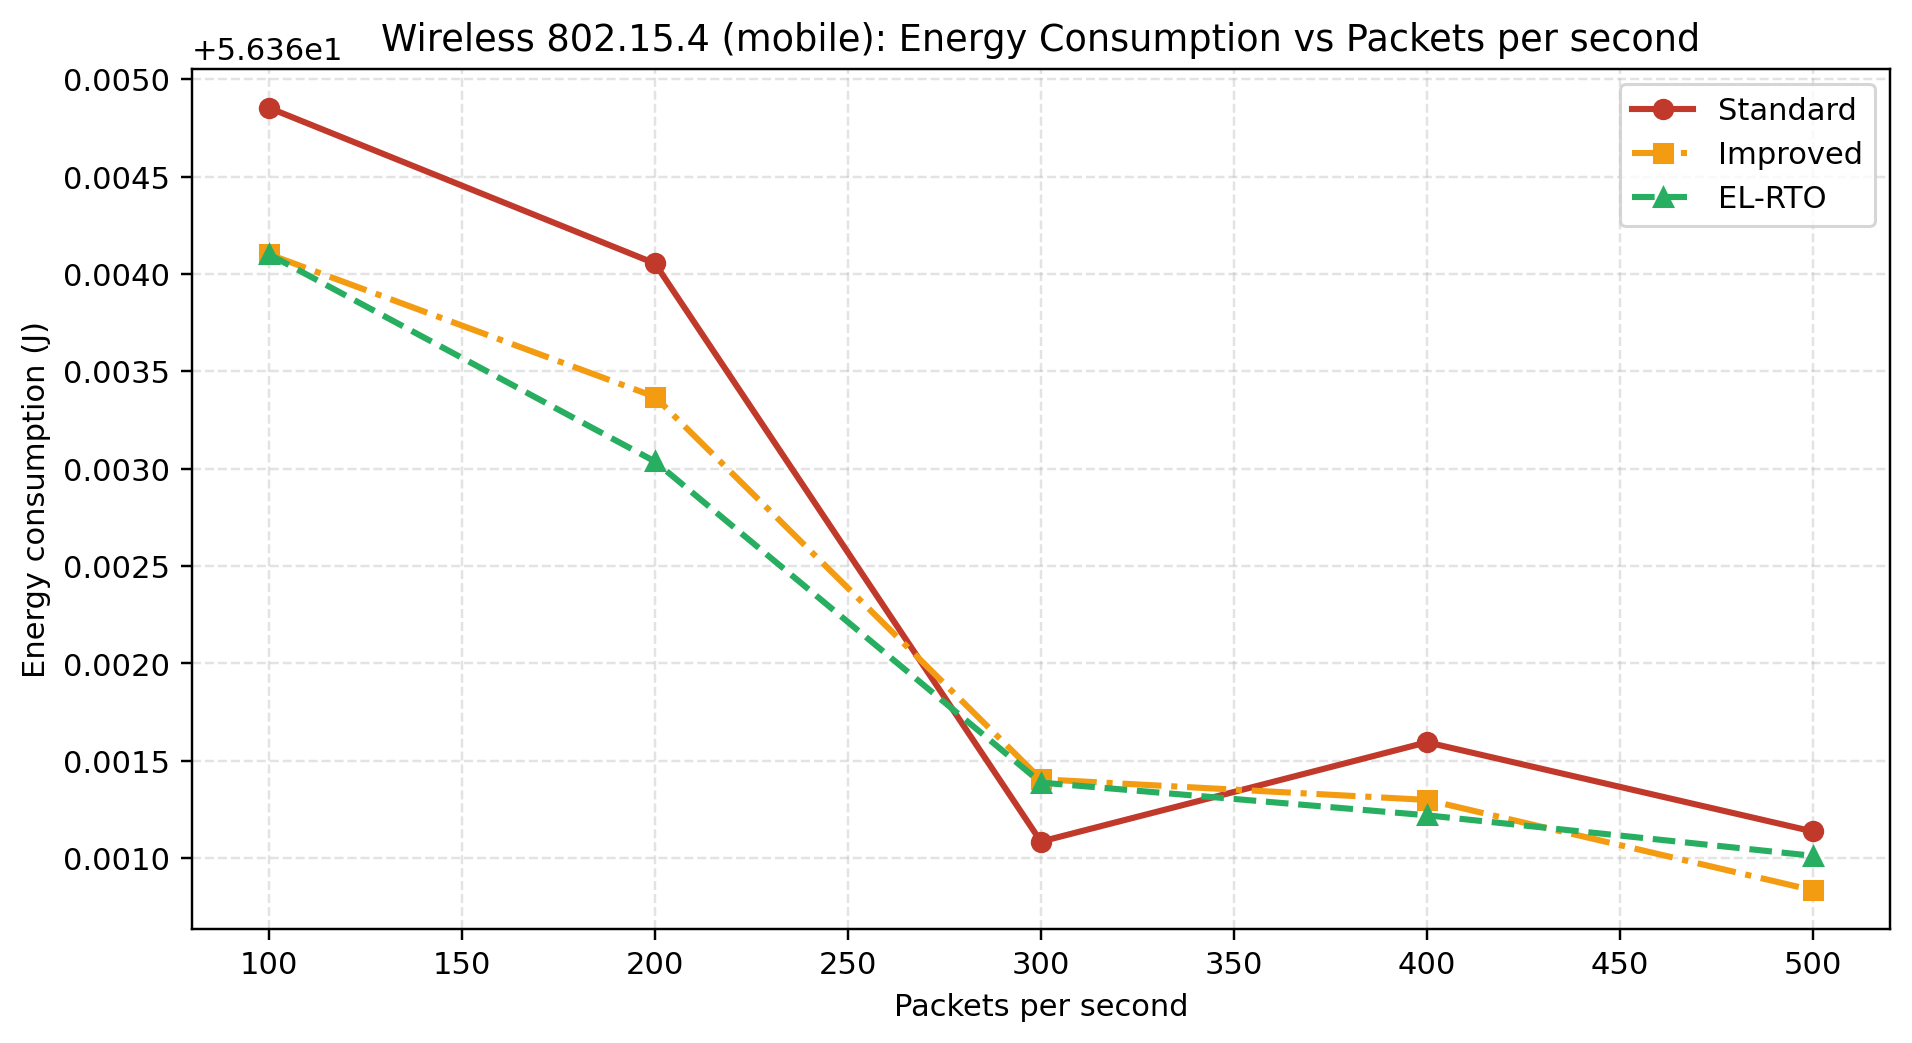
\includegraphics[width=0.47\linewidth]{2105114_final_submission/lrwpan_mobile/student2105114_lrwpan_mobile_10s_plots/lrwpan-mobile_pps_energyJ.png}
\end{frame}

\begin{frame}{LR-WPAN Mobile: Speed Sweep}
  \centering
  \begin{tabular}{cc}
    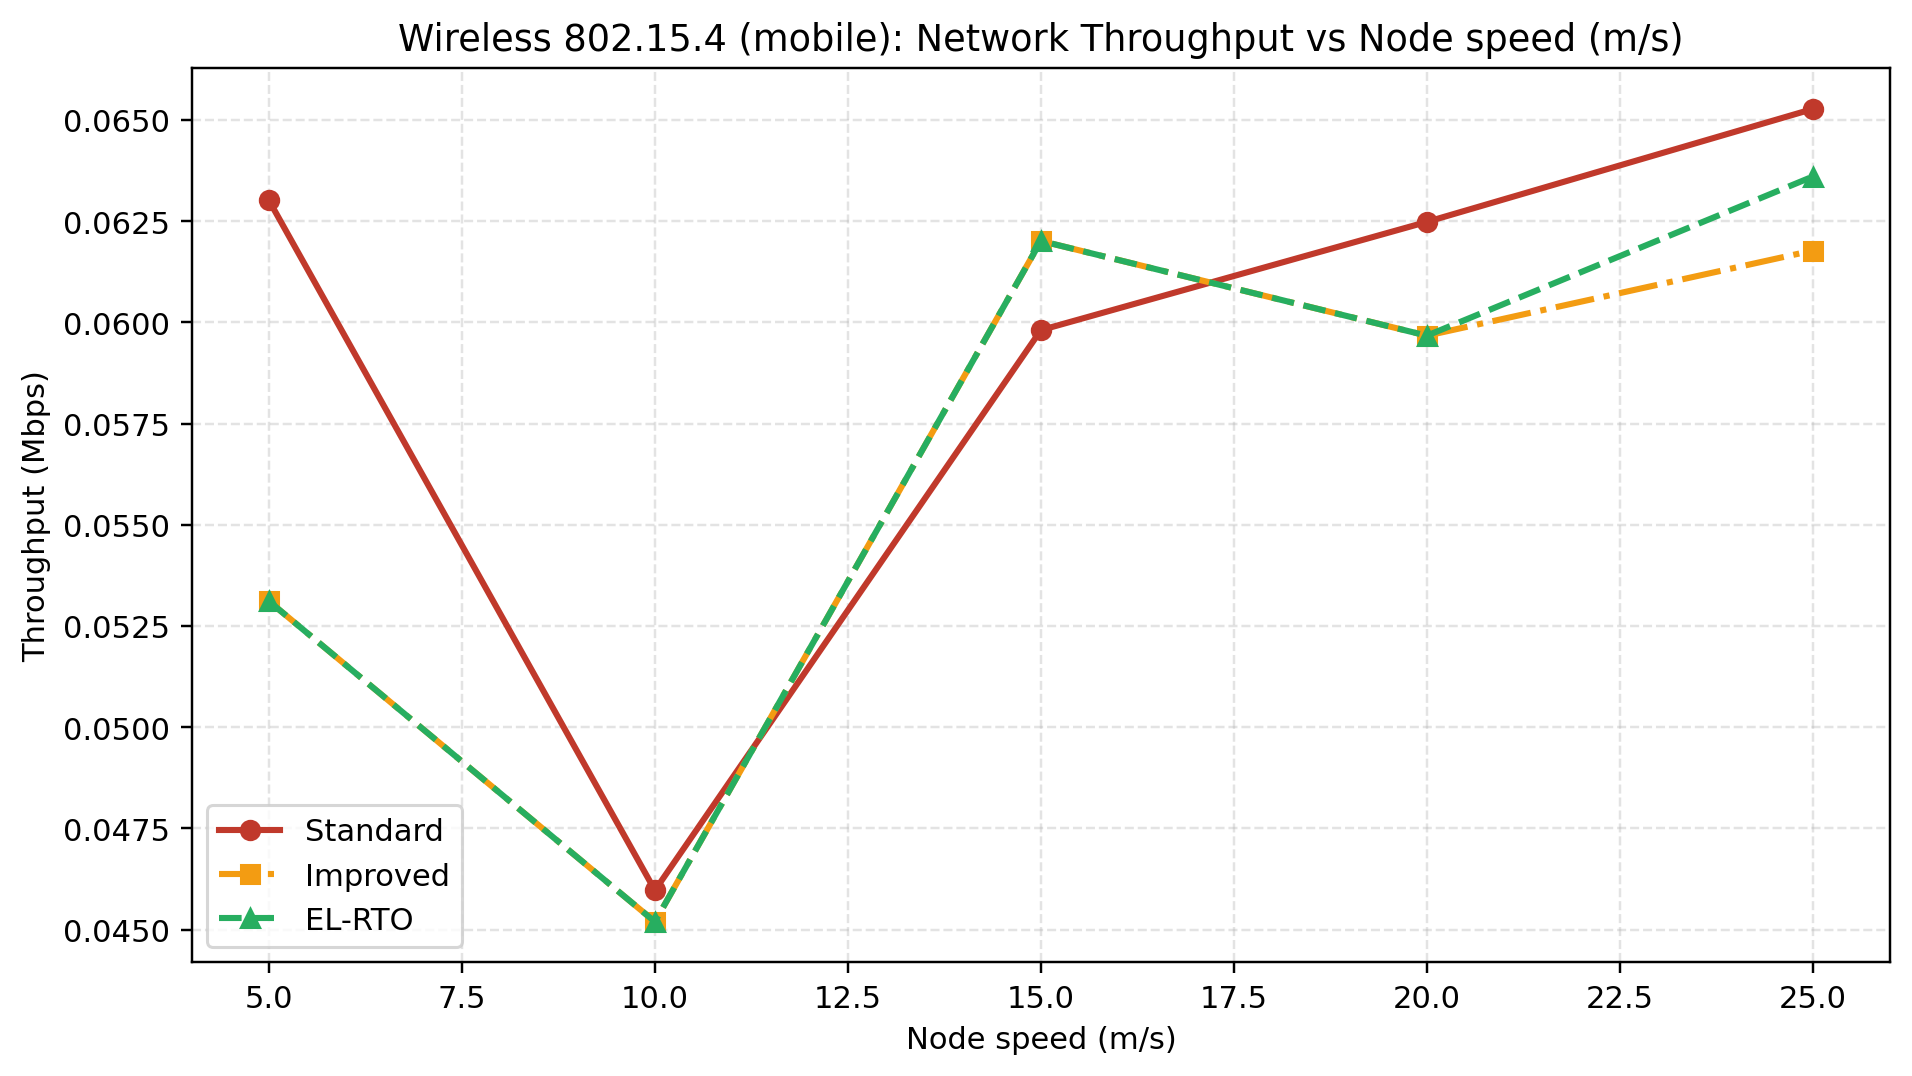
\includegraphics[width=0.47\linewidth]{2105114_final_submission/lrwpan_mobile/student2105114_lrwpan_mobile_10s_plots/lrwpan-mobile_speed_throughputMbps.png} &
    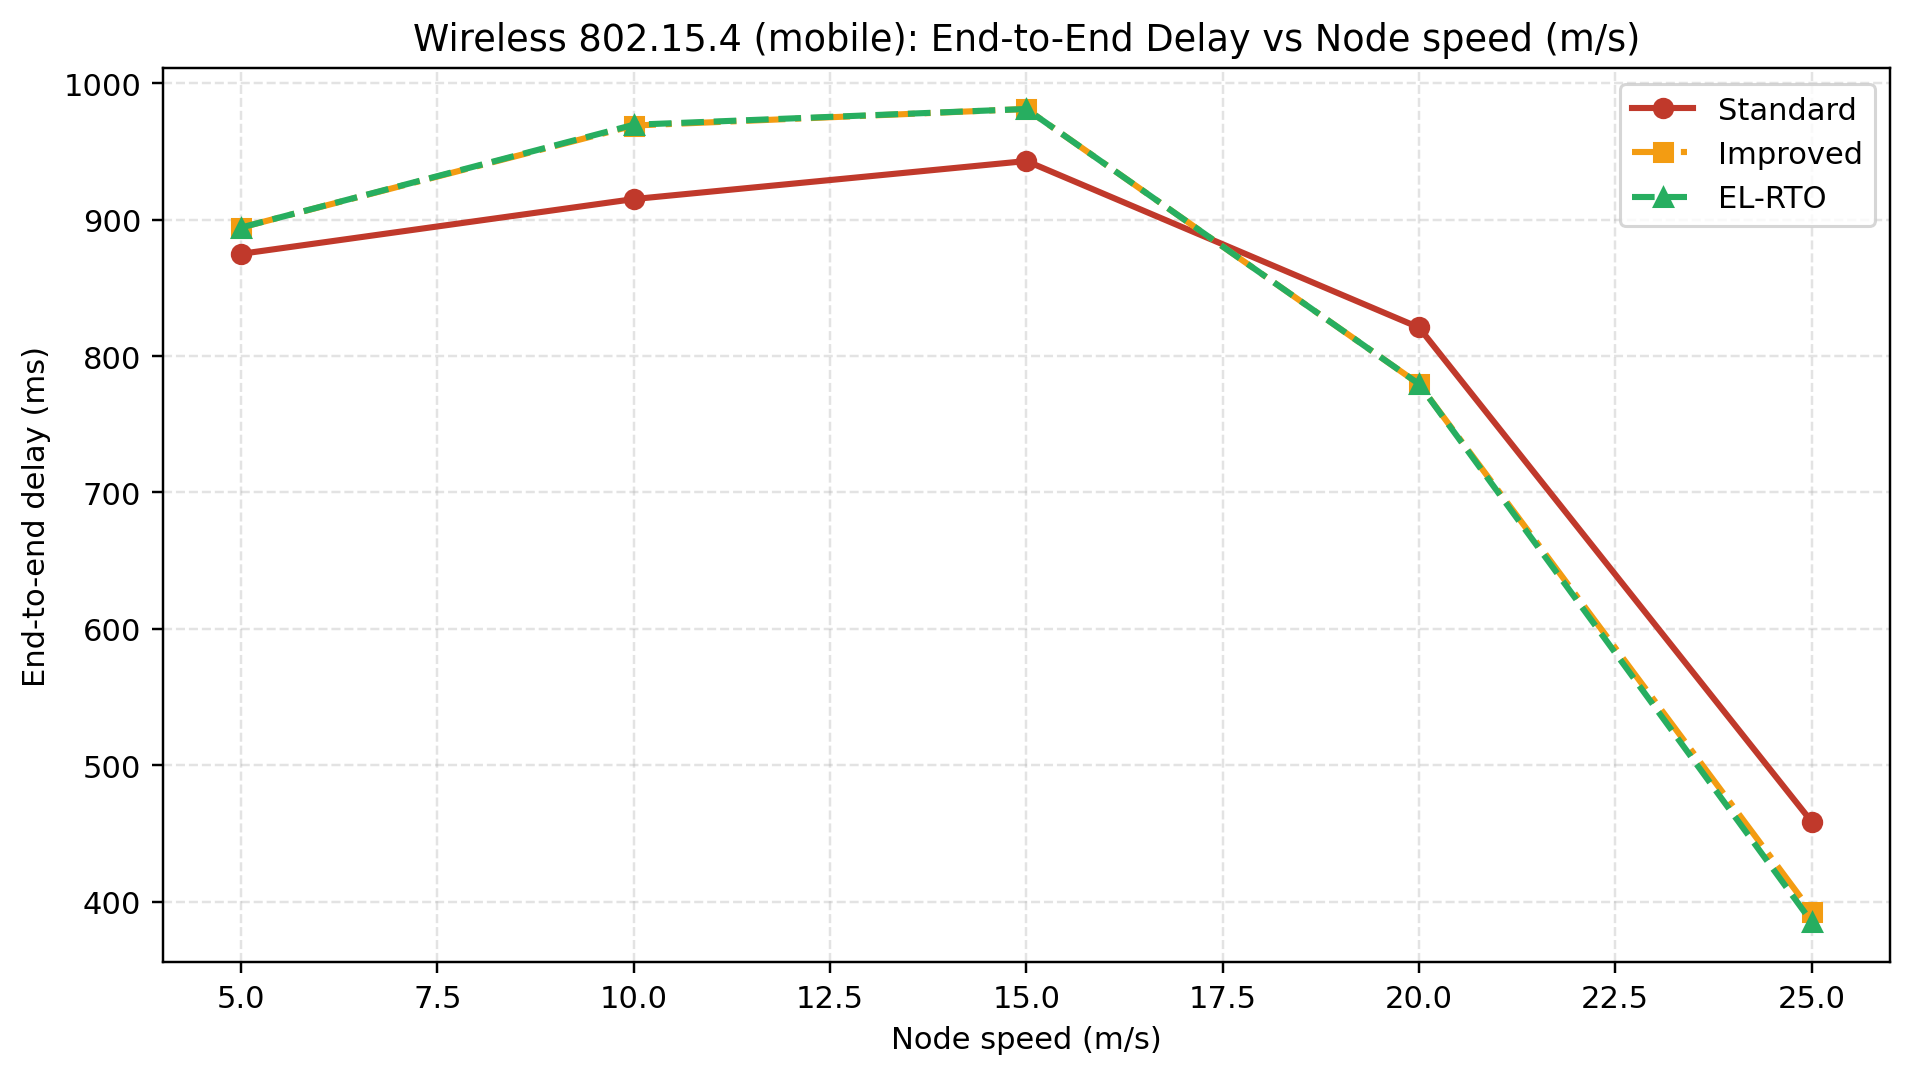
\includegraphics[width=0.47\linewidth]{2105114_final_submission/lrwpan_mobile/student2105114_lrwpan_mobile_10s_plots/lrwpan-mobile_speed_averageDelayMs.png} \\
    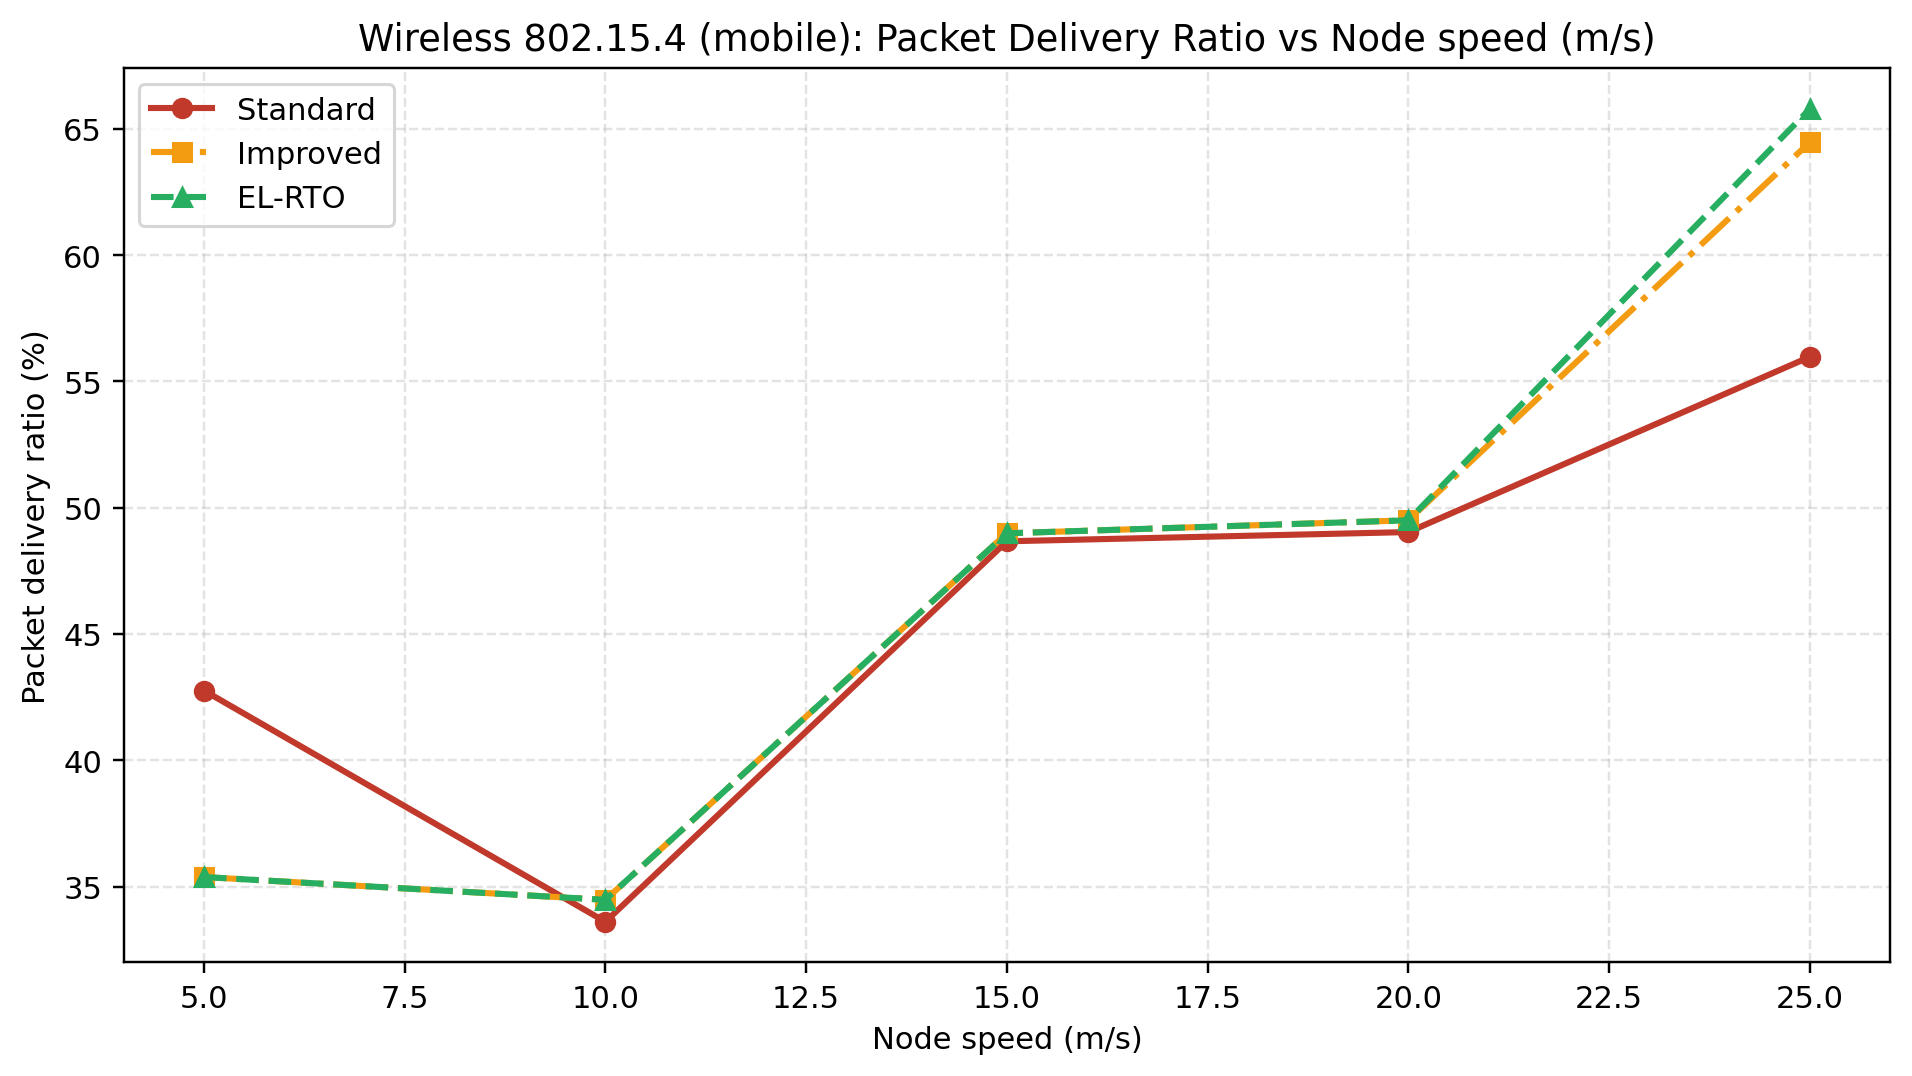
\includegraphics[width=0.47\linewidth]{2105114_final_submission/lrwpan_mobile/student2105114_lrwpan_mobile_10s_plots/lrwpan-mobile_speed_pdrPct.png} &
    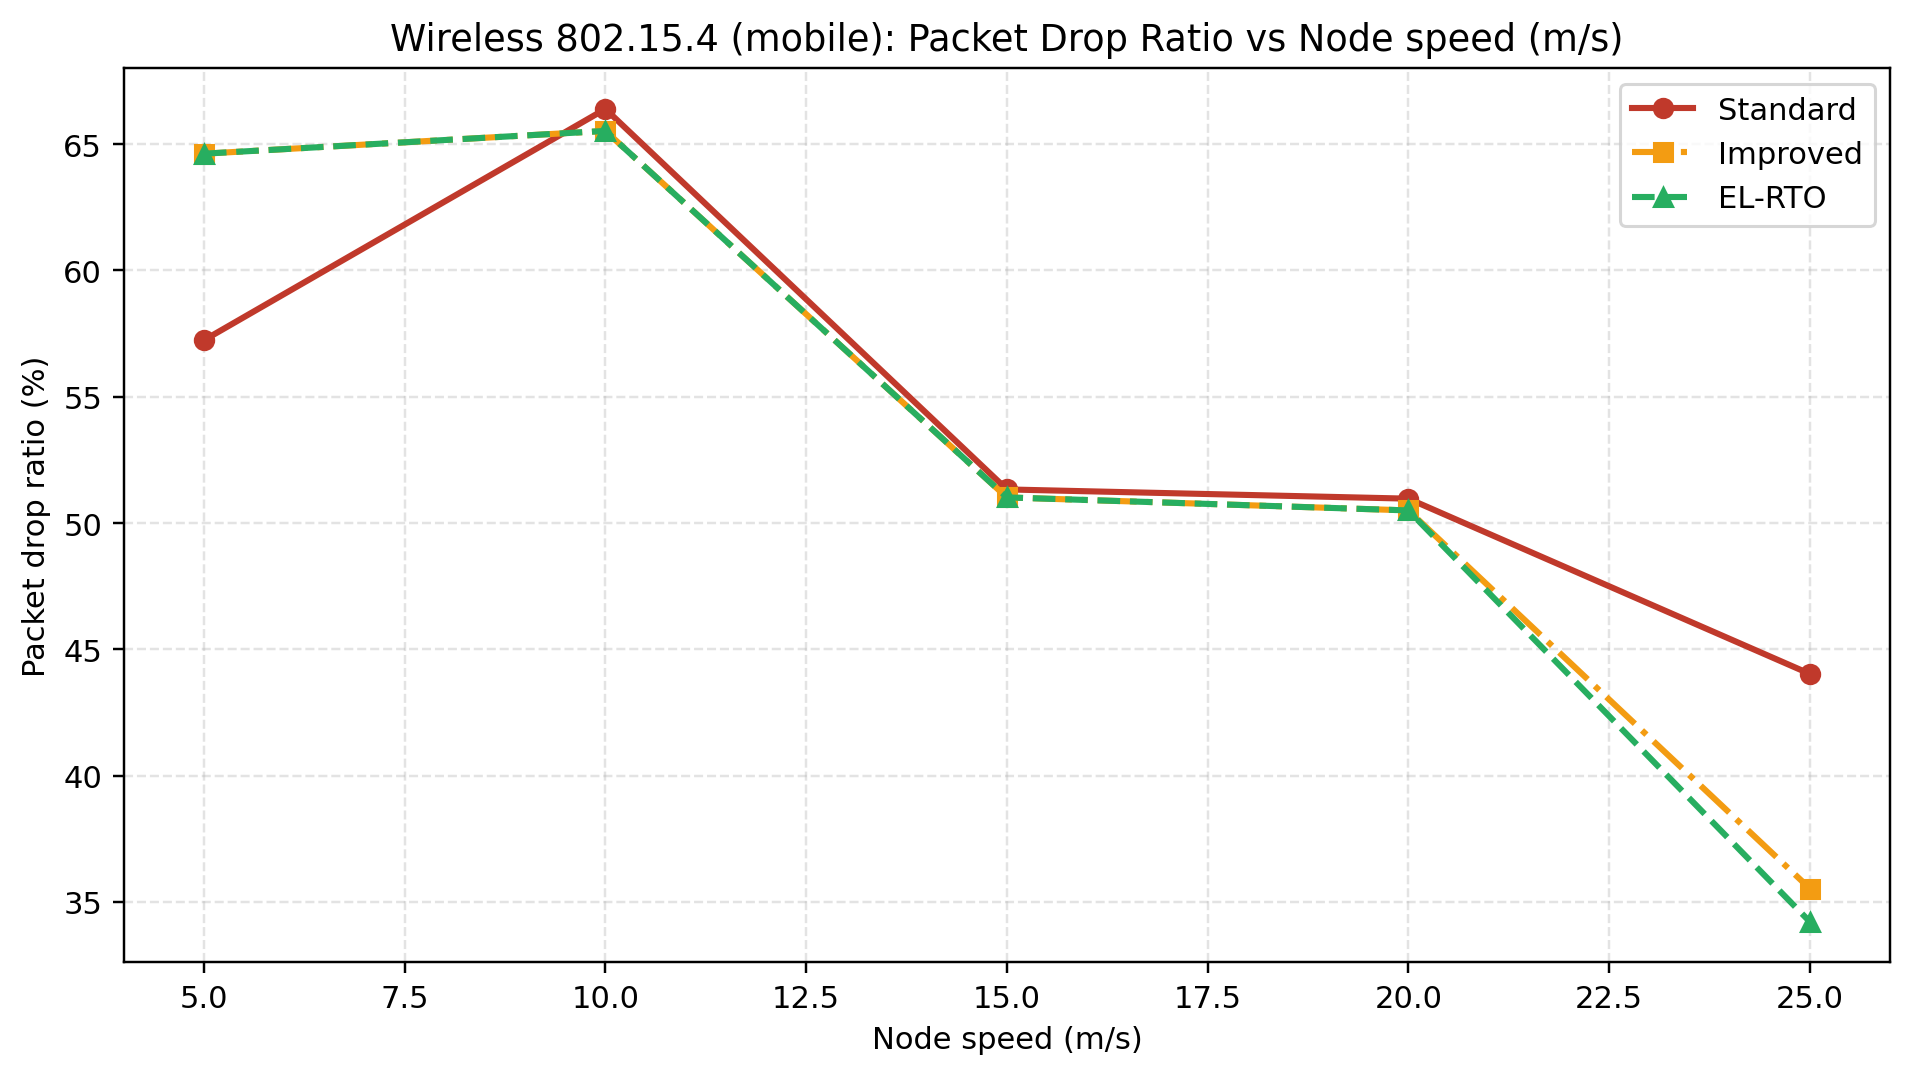
\includegraphics[width=0.47\linewidth]{2105114_final_submission/lrwpan_mobile/student2105114_lrwpan_mobile_10s_plots/lrwpan-mobile_speed_dropRatioPct.png}
  \end{tabular}

  \vspace{0.15cm}
  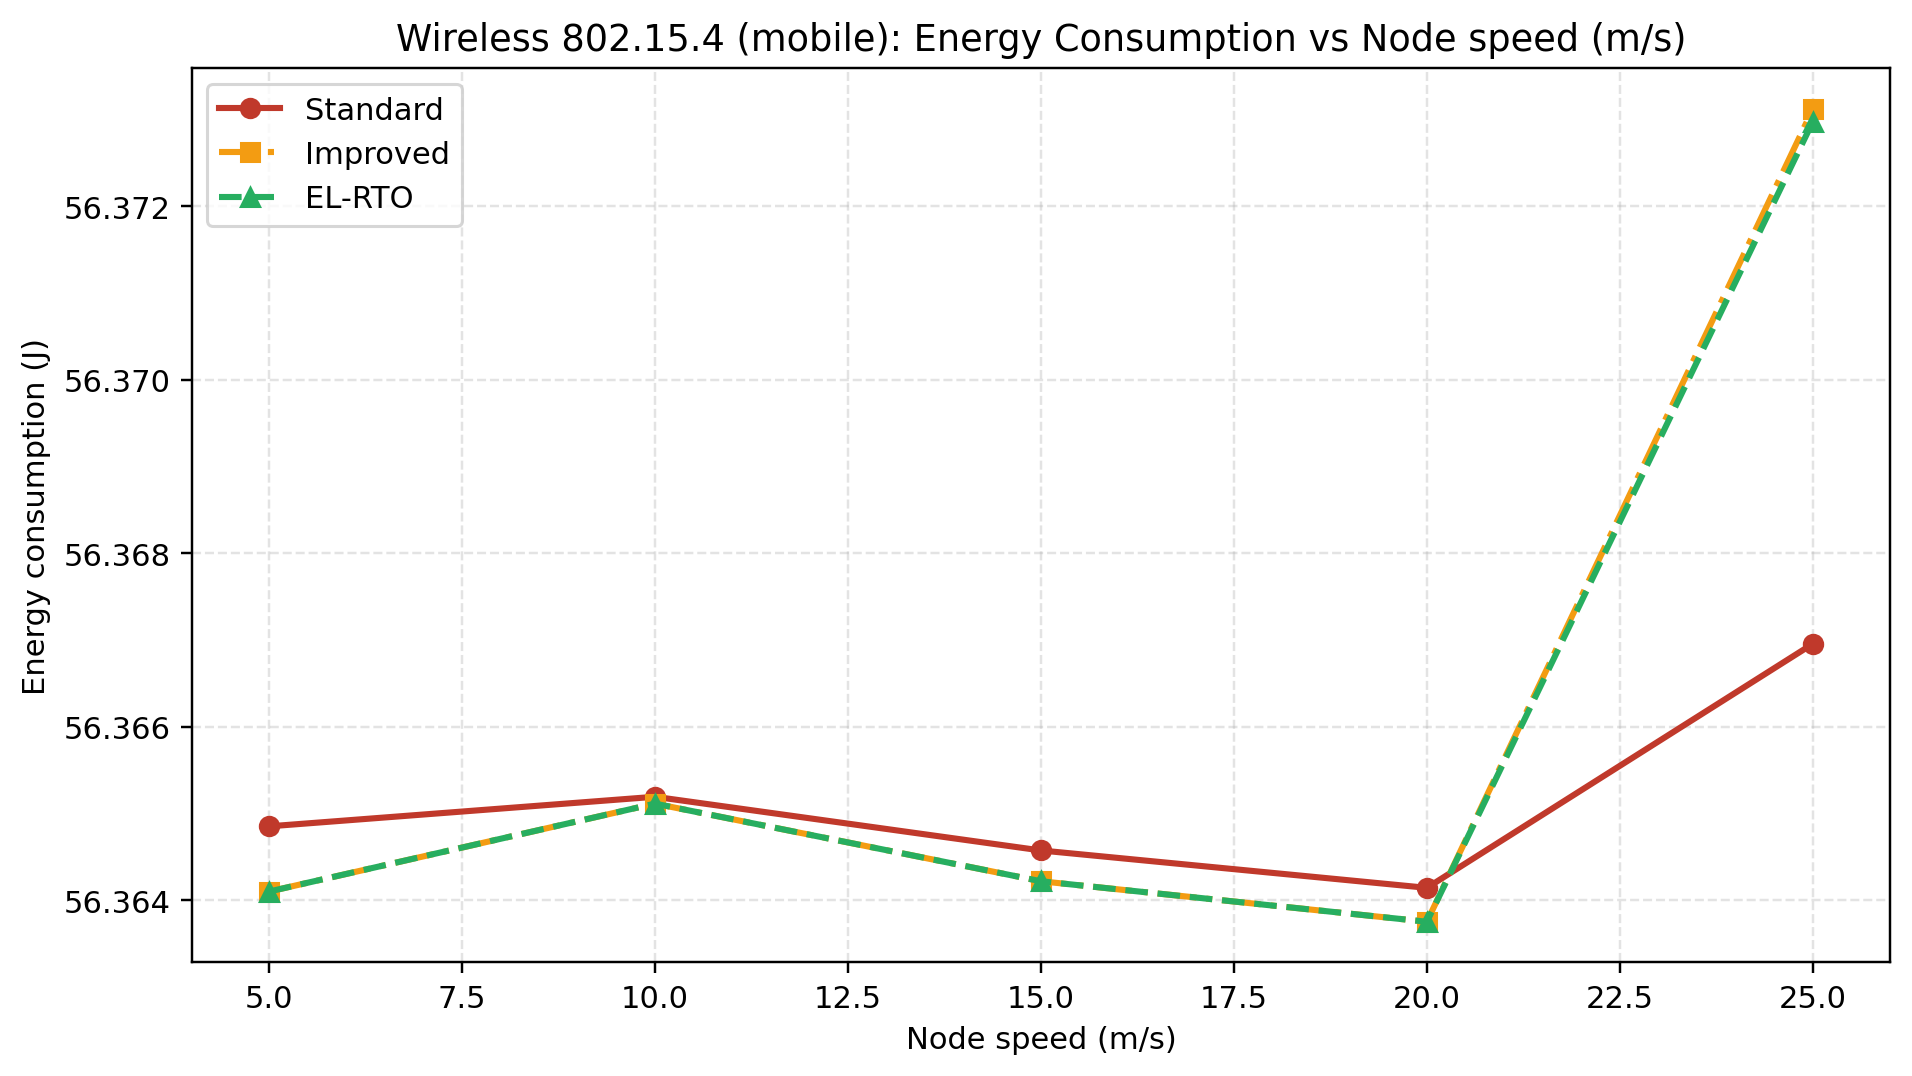
\includegraphics[width=0.47\linewidth]{2105114_final_submission/lrwpan_mobile/student2105114_lrwpan_mobile_10s_plots/lrwpan-mobile_speed_energyJ.png}
\end{frame}

\section{Conclusion}
\begin{frame}{Final Takeaway}
  \begin{itemize}
    \item ns-3 was extended to support three RTT/RTO modes:
    \begin{itemize}
      \item Standard
      \item Improved
      \item EL-RTO
    \end{itemize}
    \item The base paper behavior was reproduced in a controlled bottleneck topology.
    \item A dedicated spike experiment was built to test EL-RTO's key idea.
    \item The required checklist wireless scenarios were completed for:
    \begin{itemize}
      \item Wireless 802.11 (mobile)
      \item Wireless 802.15.4 (mobile)
    \end{itemize}
    \item Required metrics and plots were generated and organized into the final submission.
  \end{itemize}
\end{frame}

\begin{frame}{Key Files for Demonstration}
  \begin{itemize}
    \item \texttt{src/internet/model/rtt-estimator.h}
    \item \texttt{src/internet/model/rtt-estimator.cc}
    \item \texttt{scratch/rto-checklist-wireless.cc}
    \item \texttt{scratch/rto-smooth-simulation.cc}
    \item \texttt{scratch/rto-elrto-spike-simulation.cc}
    \item \texttt{2105114\_final\_submission/}
  \end{itemize}

  \vspace{0.4cm}
  \centering
  \Large Questions?
\end{frame}

\end{document}
